% Options for packages loaded elsewhere
% Options for packages loaded elsewhere
\PassOptionsToPackage{unicode}{hyperref}
\PassOptionsToPackage{hyphens}{url}
\PassOptionsToPackage{dvipsnames,svgnames,x11names}{xcolor}
%
\documentclass[
  11pt,
  letterpaper,
]{scrreprt}
\usepackage{xcolor}
\usepackage[top=1in,bottom=1in,left=1in,right=1in]{geometry}
\usepackage{amsmath,amssymb}
\setcounter{secnumdepth}{3}
\usepackage{iftex}
\ifPDFTeX
  \usepackage[T1]{fontenc}
  \usepackage[utf8]{inputenc}
  \usepackage{textcomp} % provide euro and other symbols
\else % if luatex or xetex
  \usepackage{unicode-math} % this also loads fontspec
  \defaultfontfeatures{Scale=MatchLowercase}
  \defaultfontfeatures[\rmfamily]{Ligatures=TeX,Scale=1}
\fi
\usepackage{lmodern}
\ifPDFTeX\else
  % xetex/luatex font selection
\fi
% Use upquote if available, for straight quotes in verbatim environments
\IfFileExists{upquote.sty}{\usepackage{upquote}}{}
\IfFileExists{microtype.sty}{% use microtype if available
  \usepackage[]{microtype}
  \UseMicrotypeSet[protrusion]{basicmath} % disable protrusion for tt fonts
}{}
\makeatletter
\@ifundefined{KOMAClassName}{% if non-KOMA class
  \IfFileExists{parskip.sty}{%
    \usepackage{parskip}
  }{% else
    \setlength{\parindent}{0pt}
    \setlength{\parskip}{6pt plus 2pt minus 1pt}}
}{% if KOMA class
  \KOMAoptions{parskip=half}}
\makeatother
% Make \paragraph and \subparagraph free-standing
\makeatletter
\ifx\paragraph\undefined\else
  \let\oldparagraph\paragraph
  \renewcommand{\paragraph}{
    \@ifstar
      \xxxParagraphStar
      \xxxParagraphNoStar
  }
  \newcommand{\xxxParagraphStar}[1]{\oldparagraph*{#1}\mbox{}}
  \newcommand{\xxxParagraphNoStar}[1]{\oldparagraph{#1}\mbox{}}
\fi
\ifx\subparagraph\undefined\else
  \let\oldsubparagraph\subparagraph
  \renewcommand{\subparagraph}{
    \@ifstar
      \xxxSubParagraphStar
      \xxxSubParagraphNoStar
  }
  \newcommand{\xxxSubParagraphStar}[1]{\oldsubparagraph*{#1}\mbox{}}
  \newcommand{\xxxSubParagraphNoStar}[1]{\oldsubparagraph{#1}\mbox{}}
\fi
\makeatother


\usepackage{longtable,booktabs,array}
\usepackage{calc} % for calculating minipage widths
% Correct order of tables after \paragraph or \subparagraph
\usepackage{etoolbox}
\makeatletter
\patchcmd\longtable{\par}{\if@noskipsec\mbox{}\fi\par}{}{}
\makeatother
% Allow footnotes in longtable head/foot
\IfFileExists{footnotehyper.sty}{\usepackage{footnotehyper}}{\usepackage{footnote}}
\makesavenoteenv{longtable}
\usepackage{graphicx}
\makeatletter
\newsavebox\pandoc@box
\newcommand*\pandocbounded[1]{% scales image to fit in text height/width
  \sbox\pandoc@box{#1}%
  \Gscale@div\@tempa{\textheight}{\dimexpr\ht\pandoc@box+\dp\pandoc@box\relax}%
  \Gscale@div\@tempb{\linewidth}{\wd\pandoc@box}%
  \ifdim\@tempb\p@<\@tempa\p@\let\@tempa\@tempb\fi% select the smaller of both
  \ifdim\@tempa\p@<\p@\scalebox{\@tempa}{\usebox\pandoc@box}%
  \else\usebox{\pandoc@box}%
  \fi%
}
% Set default figure placement to htbp
\def\fps@figure{htbp}
\makeatother


% definitions for citeproc citations
\NewDocumentCommand\citeproctext{}{}
\NewDocumentCommand\citeproc{mm}{%
  \begingroup\def\citeproctext{#2}\cite{#1}\endgroup}
\makeatletter
 % allow citations to break across lines
 \let\@cite@ofmt\@firstofone
 % avoid brackets around text for \cite:
 \def\@biblabel#1{}
 \def\@cite#1#2{{#1\if@tempswa , #2\fi}}
\makeatother
\newlength{\cslhangindent}
\setlength{\cslhangindent}{1.5em}
\newlength{\csllabelwidth}
\setlength{\csllabelwidth}{3em}
\newenvironment{CSLReferences}[2] % #1 hanging-indent, #2 entry-spacing
 {\begin{list}{}{%
  \setlength{\itemindent}{0pt}
  \setlength{\leftmargin}{0pt}
  \setlength{\parsep}{0pt}
  % turn on hanging indent if param 1 is 1
  \ifodd #1
   \setlength{\leftmargin}{\cslhangindent}
   \setlength{\itemindent}{-1\cslhangindent}
  \fi
  % set entry spacing
  \setlength{\itemsep}{#2\baselineskip}}}
 {\end{list}}
\usepackage{calc}
\newcommand{\CSLBlock}[1]{\hfill\break\parbox[t]{\linewidth}{\strut\ignorespaces#1\strut}}
\newcommand{\CSLLeftMargin}[1]{\parbox[t]{\csllabelwidth}{\strut#1\strut}}
\newcommand{\CSLRightInline}[1]{\parbox[t]{\linewidth - \csllabelwidth}{\strut#1\strut}}
\newcommand{\CSLIndent}[1]{\hspace{\cslhangindent}#1}



\setlength{\emergencystretch}{3em} % prevent overfull lines

\providecommand{\tightlist}{%
  \setlength{\itemsep}{0pt}\setlength{\parskip}{0pt}}



 


% --------------------------------------------------
% FastMAPOL ATBD PDF formatting
% --------------------------------------------------

\usepackage{scrlayer-scrpage}
\usepackage{xcolor}
\usepackage{booktabs}
\usepackage{longtable}
\usepackage{array}
\usepackage{microtype}

% --------------------------------------------------
% Colors
% --------------------------------------------------

\definecolor{NASABlue}{HTML}{0B3D91}
\definecolor{NASARed}{HTML}{FC3D21}
\definecolor{DarkGray}{HTML}{444444}

% --------------------------------------------------
% Headings
% --------------------------------------------------

\addtokomafont{chapter}{\color{NASABlue}}
\addtokomafont{section}{\color{NASABlue}}
\addtokomafont{subsection}{\color{DarkGray}}

% Slightly cleaner chapter heading
\RedeclareSectionCommand[
  beforeskip=0pt,
  afterskip=1.5\baselineskip
]{chapter}

% --------------------------------------------------
% Header / footer
% --------------------------------------------------

\clearpairofpagestyles

\ihead{\small FastMAPOL ATBD}
\ohead{\small PACE Mission}

\ifoot{\small NASA GSFC}
\ofoot{\small \pagemark}

\setkomafont{pageheadfoot}{\normalfont\small\color{DarkGray}}
\setkomafont{pagenumber}{\normalfont\small}

\pagestyle{scrheadings}

% --------------------------------------------------
% Tables
% --------------------------------------------------

\renewcommand{\arraystretch}{1.15}

% --------------------------------------------------
% Paragraph spacing
% --------------------------------------------------

\setlength{\parindent}{0pt}
\setlength{\parskip}{0.45em}
\makeatletter
\@ifpackageloaded{bookmark}{}{\usepackage{bookmark}}
\makeatother
\makeatletter
\@ifpackageloaded{caption}{}{\usepackage{caption}}
\AtBeginDocument{%
\ifdefined\contentsname
  \renewcommand*\contentsname{Table of contents}
\else
  \newcommand\contentsname{Table of contents}
\fi
\ifdefined\listfigurename
  \renewcommand*\listfigurename{List of Figures}
\else
  \newcommand\listfigurename{List of Figures}
\fi
\ifdefined\listtablename
  \renewcommand*\listtablename{List of Tables}
\else
  \newcommand\listtablename{List of Tables}
\fi
\ifdefined\figurename
  \renewcommand*\figurename{Figure}
\else
  \newcommand\figurename{Figure}
\fi
\ifdefined\tablename
  \renewcommand*\tablename{Table}
\else
  \newcommand\tablename{Table}
\fi
}
\@ifpackageloaded{float}{}{\usepackage{float}}
\floatstyle{ruled}
\@ifundefined{c@chapter}{\newfloat{codelisting}{h}{lop}}{\newfloat{codelisting}{h}{lop}[chapter]}
\floatname{codelisting}{Listing}
\newcommand*\listoflistings{\listof{codelisting}{List of Listings}}
\makeatother
\makeatletter
\makeatother
\makeatletter
\@ifpackageloaded{caption}{}{\usepackage{caption}}
\@ifpackageloaded{subcaption}{}{\usepackage{subcaption}}
\makeatother
\usepackage{bookmark}
\IfFileExists{xurl.sty}{\usepackage{xurl}}{} % add URL line breaks if available
\urlstyle{same}
\hypersetup{
  pdftitle={FastMAPOL Algorithm Theoretical Basis Document},
  pdfauthor={Meng Gao; Pengwang Zhai; Kamal Aryal; Kirk Knobelspiesse; Bryan Franz},
  pdfkeywords={PACE, FastMAPOL, Multi-angle Polarimetry, Aerosol, Ocean
Color, Land},
  colorlinks=true,
  linkcolor={blue},
  filecolor={Maroon},
  citecolor={blue},
  urlcolor={blue},
  pdfcreator={LaTeX via pandoc}}


% ============================================================
% FastMAPOL ATBD custom title
% ============================================================

\title{%
\begin{tabular}{c}
\includegraphics[height=1.15in]{logo/nasa_logo.png}
\\[0.7cm]
{\LARGE\bfseries FastMAPOL Algorithm Theoretical Basis Document}
\\[0.35cm]
{\large\normalfont Coupled Aerosol, Ocean, and Land Retrievals from PACE
Multi-Angle Polarimetry}
\\[0.45cm]
{\normalsize\normalfont NASA PACE Mission}
\end{tabular}%
}

% Authors are included in the metadata table below
\author{}

\date{%
{\normalsize\normalfont
\renewcommand{\arraystretch}{1.45}%
\begin{tabular}{@{}r@{\hspace{0.45cm}}l@{}}
\textbf{Authors} &
Meng Gao, \quad Pengwang Zhai, \quad Kamal Aryal, \quad Kirk
Knobelspiesse, \quad Bryan Franz \\
\textbf{POC} &
Meng Gao \;(\href{mailto:meng.gao@nasa.gov}{meng.gao@nasa.gov}) \\
\textbf{Keywords} &
PACE \textperiodcentered\ FastMAPOL \textperiodcentered\ Multi-angle
Polarimetry \textperiodcentered\ Aerosol \textperiodcentered\ Ocean
Color \textperiodcentered\ Land \\
\textbf{Website} &
%%\href{https://fastmapol.github.io/mapol-doc/}{FastMAPOL ATBD} \\
\url{https://fastmapol.github.io/mapol-doc/} \\
\textbf{Version} & 0.3 \\
\textbf{Date} & 2026-09-03 \\
\end{tabular}%
}%
}
\begin{document}
\maketitle

\renewcommand*\contentsname{Table of contents}
{
\hypersetup{linkcolor=}
\setcounter{tocdepth}{2}
\tableofcontents
}
\listoffigures
\listoftables

\bookmarksetup{startatroot}

\chapter*{About This Document}\label{about-this-document}
\addcontentsline{toc}{chapter}{About This Document}

\markboth{About This Document}{About This Document}

This Algorithm Theoretical Basis Document (ATBD) describes the
theoretical basis, implementation, data products, and validation of the
Fast Multi-Angle Polarimetric Ocean and Land (FastMAPOL) retrieval
algorithm developed for the NASA Plankton, Aerosol, Cloud, ocean
Ecosystem (PACE) mission.

FastMAPOL retrieves aerosol, ocean, and land surface properties from
multi-angle polarimetric observations acquired by the PACE polarimeters,
HARP2 and SPEXone. The algorithm is currently run in production and
produce operational aerosol, ocean color and land surface products with
public available data through NASA Earth Data Cloud.

The following chapters provide information on data access through NASA
Earthdata and product release notes. These are followed by
\textbf{FastMAPOL at a Glance}, which provides a high-level overview of
the algorithm. The algorithm overview, data product format, and
validation results are then summarized in the subsequent chapters. More
detailed technical descriptions of the algorithm and its underlying
methodology are provided in the second part of this document.

A web version of this document is available at
\href{https://fastmapol.github.io/mapol-doc/}{FastMAPOL ATBD} and may
provide more timely updates. Both the web content and the link location
are subject to change. Please contact the authors for the latest
information.

\section*{Document Information}\label{document-information}

\markright{Document Information}

\begin{longtable}[]{@{}
  >{\raggedright\arraybackslash}p{(\linewidth - 2\tabcolsep) * \real{0.5000}}
  >{\raggedright\arraybackslash}p{(\linewidth - 2\tabcolsep) * \real{0.5000}}@{}}
\toprule\noalign{}
\endhead
\bottomrule\noalign{}
\endlastfoot
\textbf{Mission} & PACE \\
\textbf{Point of Contact} & Meng Gao
(\href{mailto:meng.gao@nasa.gov}{\nolinkurl{meng.gao@nasa.gov}}) \\
\textbf{Keywords} & PACE · FastMAPOL · Multi-angle Polarimetry · Aerosol
· Ocean Color · Land \\
\textbf{Website} & \url{https://fastmapol.github.io/mapol-doc/} \\
\textbf{Version} & 0.3 \\
\end{longtable}

\section*{How to Cite}\label{how-to-cite}

\markright{How to Cite}

When using or referring to FastMAPOL ATBD, please cite this document as:

\begin{quote}
Gao, M., P. Zhai, K. Aryal, K. Knobelspiesse, and B. Franz.
\emph{FastMAPOL Algorithm Theoretical Basis Document: Coupled Aerosol,
Ocean, and Land Retrievals from PACE Multi-Angle Polarimetry}. NASA
Goddard Space Flight Center, Version 0.3, 2026.
\textless{}https://fastmapol.github.io/mapol-doc/\textgreater{}
\end{quote}

Please also cite the relevant peer-reviewed publications when using the
algorithm or data products.

\bookmarksetup{startatroot}

\chapter*{Earthdata Access}\label{earthdata-access}
\addcontentsline{toc}{chapter}{Earthdata Access}

\markboth{Earthdata Access}{Earthdata Access}

FastMAPOL Level-2 (L2) and Level-3 mapped (L3M) products are distributed
through NASA Earthdata. The most recent production version is listed
first below.

\section*{Version 4.0}\label{version-4.0}
\addcontentsline{toc}{section}{Version 4.0}

\markright{Version 4.0}

\textbf{SPEXone MAPOL\_OCEAN}

\begin{itemize}
\tightlist
\item
  \textbf{L2:}
  \url{https://doi.org/10.5067/PACE/SPEXONE/L2/MAPOL_OCEAN/4.0}
\item
  \textbf{L3M:}
  \url{https://doi.org/10.5067/PACE/SPEXONE/L3M/MAPOL_OCEAN/4.0}
\end{itemize}

\textbf{HARP2 MAPOL\_OCEAN}

\begin{itemize}
\tightlist
\item
  \textbf{L2:}
  \url{https://doi.org/10.5067/PACE/HARP2/L2/MAPOL_OCEAN/4.0}
\item
  \textbf{L3M:}
  \url{https://doi.org/10.5067/PACE/HARP2/L3M/MAPOL_OCEAN/4.0}
\end{itemize}

\textbf{HARP2 MAPOL\_LAND}

\begin{itemize}
\tightlist
\item
  \textbf{L2:}
  \url{https://doi.org/10.5067/PACE/HARP2/L2/MAPOL_LAND/4.0}
\item
  \textbf{L3M:}
  \url{https://doi.org/10.5067/PACE/HARP2/L3M/MAPOL_LAND/4.0}
\end{itemize}

\section*{Version 3.0}\label{version-3.0}
\addcontentsline{toc}{section}{Version 3.0}

\markright{Version 3.0}

Version 3.0 products remain available for users who need access to the
earlier FastMAPOL production release.

\textbf{SPEXone MAPOL\_OCEAN}

\begin{itemize}
\tightlist
\item
  \textbf{L2:}
  \url{https://doi.org/10.5067/PACE/SPEXONE/L2/MAPOL_OCEAN/3.0}
\item
  \textbf{L2:}
  \url{https://doi.org/10.5067/PACE/SPEXONE/L3M/MAPOL_OCEAN/3.0}
\end{itemize}

\textbf{HARP2 MAPOL\_OCEAN}

\begin{itemize}
\tightlist
\item
  \textbf{L2:}
  \url{https://doi.org/10.5067/PACE/HARP2/L2/MAPOL_OCEAN/3.0}
\item
  \textbf{L3M:}
  \url{https://doi.org/10.5067/PACE/HARP2/L3M/MAPOL_OCEAN/3.0}
\end{itemize}

\bookmarksetup{startatroot}

\chapter*{Release Notes}\label{release-notes}
\addcontentsline{toc}{chapter}{Release Notes}

\markboth{Release Notes}{Release Notes}

The FastMAPOL SPEXone release notes are available under
\href{https://www.earthdata.nasa.gov/data/catalog/ob-cloud-pace-spexone-l2-mapol-ocean-4.0\#documents-and-resources}{Documents
and Resources on the Earthdata SPEXone product pages}. The FastMAPOL
HARP2 release notes are similarly available under
\href{https://www.earthdata.nasa.gov/data/catalog/ob-cloud-pace-harp2-l2-mapol-ocean-4.0\#documents-and-resources}{Documents
and Resources on the Earthdata HARP2 product pages}.

The PACE release notes available through the
\href{https://pace.oceansciences.org/access_pace_data.htm}{PACE Data
Access page} may not always contain the most up-to-date product-specific
information.

Because these links are subject to change, the relevant release
information is also provided below for reference.

\section*{Version 4.0}\label{version-4.0-1}
\addcontentsline{toc}{section}{Version 4.0}

\markright{Version 4.0}

\subsection*{HARP2 Level-2 Products}\label{harp2-level-2-products}

\begin{itemize}
\item
  \texttt{MAPOL\_LAND} (Aerosol and Land Properties, FastMAPOL
  Algorithm)
\item
  \texttt{MAPOL\_OCEAN} (Aerosol and Ocean Properties, FastMAPOL
  Algorithm)
\end{itemize}

\textbf{Changes from Version 3}

\begin{itemize}
\item
  Uses Version 4 L1C data, with the same FastMAPOL retrieval algorithm
  previously applied to Version 3 data.
\item
  Aerosol retrieval quality is improved for the \texttt{MAPOL\_OCEAN}
  data suites. Quality flags 0 and 1 are recommended for scientific
  applications.
\item
  Quality flag definitions have been updated. Please refer to the new
  HelpHub notebooks for details:

  \url{https://nasa.github.io/oceandata-notebooks/sections/cloud-atmosphere.html}
\item
  Ocean surface reflectance products \texttt{Rrs1} and \texttt{Rrs2}
  have been renamed \texttt{Rrs\_angular} and \texttt{Rrs\_nadir},
  respectively. These represent angular Rrs before and after BRDF
  correction.
\item
  New \texttt{MAPOL\_LAND} data suites have been added. Multi-angle land
  surface reflectances are reported as rhos\_angular and rhos\_nadir.
\end{itemize}

\textbf{Known issues}

\begin{itemize}
\item
  A substantial fraction of aerosol retrievals is associated with
  lower-quality retrieval conditions, including larger \(\chi^2\) values
  and fewer valid viewing angles (\texttt{nv\_ref} and
  \texttt{nv\_dolp}). These retrievals can exhibit larger biases in
  aerosol optical properties such as AOD. Users are encouraged to apply
  the recommended quality flags.
\item
  \texttt{MAPOL\_LAND} is undergoing active testing and improvement. The
  current version shows significant biases in both fine- and coarse-mode
  aerosol properties and should therefore be used with caution.
\end{itemize}

\subsection*{HARP2 Level-3 Products}\label{harp2-level-3-products}

HARP2 Level-2 products are composited into global Level-3 binned and
mapped products. Daily, 8-day, and monthly Level-3 mapped products are
produced on an equirectangular grid at 0.1-deg and 1-deg resolution. The
available list of mapped product types now include:

\begin{itemize}
\tightlist
\item
  \texttt{MAPOL\_OCEAN}: aerosol and ocean properties from FastMAPOL
  algorithm
\item
  \texttt{MAPOL\_LAND}: aerosol and land properties from FastMAPOL
  algorithm
\end{itemize}

\subsection*{SPEXone Level-2 Products}\label{spexone-level-2-products}

\textbf{Changes from Version 3}

\begin{itemize}
\item
  Uses Version 4 L1C data, with the same FastMAPOL retrieval algorithm
  previously applied to Version 3 data.
\item
  Retrieval performance is similar to the reported validation results
  against AERONET and AERONET-OC observations (Gao, M., K. Aryal, P.
  Zhai, K. Knobelspiesse, B. Franz, B. Cairns, I. Cetinić, G. Fu, O.
  Hasekamp, A. Ibrahim, A. M. Sayer, and P. J. Werdell. 2026. ``Where
  Sky Meets Sea: Integrated Aerosol and Ocean Color Retrieval from PACE
  SPEXone Multi-Angle Polarimetry.'' \emph{Remote Sensing of
  Environment}, 345, 115603.
  \url{https://doi.org/10.1016/j.rse.2026.115603}).
\item
  \texttt{Rrs1} and \texttt{Rrs2} have been renamed
  \texttt{Rrs\_angular} and \texttt{Rrs\_nadir}, respectively,
  representing angular Rrs before and after BRDF correction.
\end{itemize}

\textbf{Known issues}

\begin{itemize}
\item
  Ocean Rrs bias is reduced, but still with a positive bias of
  approximately 0.001 sr⁻¹ in the blue bands.
\item
  Over coastal waters, Rrs and AOD exhibit stronger coupling and higher
  retrieval uncertainties, as discussed in the above paper. Improvements
  are planned to better account for complex water optical properties
  (Aryal, K., M. Gao, P. Zhai, B. A. Franz, K. Knobelspiesse, A.
  Ibrahim, and J. Werdell. 2026. ``Aerosol and Ocean Color Retrievals
  from the FastMAPOL/Component Algorithm Using NASA's PACE Polarimetric
  Measurements.'' \emph{Optics Express}, 34(16), 29139.
  \url{https://doi.org/10.1364/OE.607432}).
\end{itemize}

\subsection*{SPEXone Level-3 Products}\label{spexone-level-3-products}

SPEXone Level-2 products are composited into global Level-3 binned and
mapped products. Daily, 8-day, and monthly Level-3 mapped products are
produced on an equirectanular grid at 0.1-deg and 1-deg resolution. The
available list of mapped product types now include:

\begin{itemize}
\tightlist
\item
  \texttt{MAPOL\_OCEAN}: aerosol and ocean properties from FastMAPOL
  algorithm
\end{itemize}

\section*{Version 3.0}\label{version-3.0-1}
\addcontentsline{toc}{section}{Version 3.0}

\markright{Version 3.0}

\subsection*{SPEXone Level-2 Products}\label{spexone-level-2-products-1}

\begin{itemize}
\tightlist
\item
  \texttt{MAPOL\_OCEAN} (Aerosol and Ocean Properties from FastMAPOL
  Algorithm)
\end{itemize}

This is the first release of Level-2 and Level-3 products from the
FastMAPOL algorithm as applied to SPEXone Version 3 Level-1C. The
FastMAPOL algorithm generates a large suite of aerosol and ocean
properties. A subset is listed here.

\textbf{Provisional Products}

\begin{itemize}
\tightlist
\item
  Aerosol Optical Thickness (\texttt{aot})
\item
  Single Scattering Albedo (\texttt{ssa})
\item
  Effective Radius of Fine Mode Aerosols (\texttt{reff\_fine})
\item
  Effective Radius of Coarse Mode Aerosols (\texttt{reff\_fine})
\item
  Fine Mode Fraction (\texttt{fmf})
\item
  Fine Mode Fraction by Volume (\texttt{fvf})
\item
  Real Index of Refraction (\texttt{mr})
\item
  Imaginary Index of Refraction (\texttt{mi})
\item
  Wind speed (\texttt{wind\_speed})
\item
  Chlorophyll a concentration (\texttt{chla})
\item
  Angular Mean Water-Leaving Reflectance before BRDF correction
  (\texttt{Rrs1\_mean})
\item
  Standard Deviation of Rrs1 (\texttt{Rrs1\_std})
\item
  Angular Mean Water-Leaving Reflectance after BRDF correction
  (\texttt{Rrs2\_mean})
\item
  Standard Deviation of Rrs2 (\texttt{Rrs2\_std})
\end{itemize}

\textbf{Known issues}

\begin{itemize}
\tightlist
\item
  Small negative Rrs offset (\textasciitilde-0.001) is often observed at
  wavelengths \textgreater{} 600 nm.
\item
  BRDF correction does not fully remove Rrs angular dependence (as seen
  in Rrs2).
\item
  High Rrs bias at 678 nm likely due to influence of the Oxygen A-band.
\end{itemize}

\subsection*{SPEXone Level-3 Products}\label{spexone-level-3-products-1}

SPEXone Level-2 products are composited into global Level-3 binned and
mapped products. Daily, 8-day, and monthly Level-3 mapped products are
produced on an equirectanular grid at 0.1-deg and 1-deg resolution. The
available list of mapped product types now include:

\begin{itemize}
\tightlist
\item
  \texttt{MAPOL\_OCEAN}: aerosol and ocean properties over ocean from
  FastMAPOL algorithm
\end{itemize}

\subsection*{HARP2 Level-2 Products}\label{harp2-level-2-products-1}

\begin{itemize}
\tightlist
\item
  \texttt{MAPOL\_OCEAN} (Aerosol and Ocean Properties from FastMAPOL
  Algorithm)
\end{itemize}

This is the first release of Level-2 and Level-3 products from the
FastMAPOL algorithm as applied to HARP2 Version 3 Level-1C. The
FastMAPOL algorithm generates a large suite of aerosol and ocean optical
properties. A subset is listed here.

\textbf{Provisional Products}

\begin{itemize}
\tightlist
\item
  Aerosol Optical Thickness (\texttt{aot})
\item
  Single Scattering Albedo (\texttt{ssa})
\item
  Effective Radius of Fine Mode Aerosols (\texttt{reff\_fine})
\item
  Effective Radius of Coarse Mode Aerosols (\texttt{reff\_fine})
\item
  Fine Mode Fraction (\texttt{fmf})
\item
  Fine Mode Fraction by Volume (\texttt{fvf})
\item
  Real Index of Refraction (\texttt{mr})
\item
  Imaginary Index of Refraction (\texttt{mi})
\item
  Wind speed (\texttt{wind\_speed})
\item
  Chlorophyll a concentration (\texttt{chla})
\item
  Angular Mean Water-Leaving Reflectance before BRDF correction
  (\texttt{Rrs1\_mean})
\item
  Standard Deviation of Rrs1 (\texttt{Rrs1\_std})
\item
  Angular Mean Water-Leaving Reflectance after BRDF correction
  (\texttt{Rrs2\_mean})
\item
  Standard Deviation of Rrs2 (\texttt{Rrs2\_std})
\end{itemize}

\textbf{Known issues}

\begin{itemize}
\tightlist
\item
  Aerosol optical depth is biased high (\textasciitilde0.07) as compared
  with AERONET-OC.
\item
  Remote-sensing reflectance (Rrs) is biased low (-0.001) as compared
  with AERONET-OC.
\item
  High uncertainty in aerosol microphysical retrievals (mr, mi, sph, alh
  etc).
\item
  Fewer polarization measurements than radiance measurements are
  successfully fitted, as indicated by valid angle counts (Nv\_ref and
  Nv\_dolp) and angular data mask (mask\_ref and mask\_dolp).
\end{itemize}

\subsection*{HARP2 Level-3 Products}\label{harp2-level-3-products-1}

HARP2 Level-2 products are composited into global Level-3 binned and
mapped products. Daily, 8-day, and monthly Level-3 mapped products are
produced on an equirectanular grid at 0.1-deg and 1-deg resolution. The
available list of mapped product types now include:

\begin{itemize}
\tightlist
\item
  \texttt{MAPOL\_OCEAN}: aerosol and ocean properties over ocean from
  FastMAPOL algorithm
\end{itemize}

\bookmarksetup{startatroot}

\chapter*{Jupyter Notebook Tutorials}\label{jupyter-notebook-tutorials}
\addcontentsline{toc}{chapter}{Jupyter Notebook Tutorials}

\markboth{Jupyter Notebook Tutorials}{Jupyter Notebook Tutorials}

FastMAPOL products (\texttt{MAPOL\_OCEAN} and \texttt{MAPOL\_LAND}) can
be accessed and explored using NASA's \texttt{earthaccess} Python
package, which provides tools for discovering and accessing data through
NASA Earthdata. The following tutorials from PACE Help Hub demonstrate
how to search for, download, analyze, and visualize the data products
using Jupyter notebooks.

These notebook tutorials are available through the
\href{https://nasa.github.io/oceandata-notebooks/sections/cloud-atmosphere.html}{PACE
Help Hub}.

\begin{itemize}
\tightlist
\item
  \href{https://nasa.github.io/oceandata-notebooks/notebooks/harp2/harp2_l2_fastmapol_aerosol_ocean_product.html}{HARP2
  Ocean Aerosols (FastMAPOL)} - Working with aerosol data over ocean
  from the HARP2 polarimeter with the FastMAPOL algorithm
\item
  \href{https://nasa.github.io/oceandata-notebooks/notebooks/harp2/harp2_l2_fastmapol_aerosol_land_product.html}{HARP2
  Land Aerosols (FastMAPOL)} - Working with aerosol data over land from
  the HARP2 polarimeter with the FastMAPOL algorithm
\item
  \href{https://nasa.github.io/oceandata-notebooks/notebooks/spexone/spexone_l2_fastmapol_aerosol_product.html}{SPEXone
  Aerosols (FastMAPOL)} - Analyzing aerosol retrievals over ocean from
  SPEXone measurements with the FastMAPOL algorithm
\end{itemize}

\bookmarksetup{startatroot}

\chapter*{Data Visualization with
SeaDAS}\label{data-visualization-with-seadas}
\addcontentsline{toc}{chapter}{Data Visualization with SeaDAS}

\markboth{Data Visualization with SeaDAS}{Data Visualization with
SeaDAS}

FastMAPOL products can also be accessed, explored, and visualized using
NASA's Sea, Earth, Atmosphere Data Analysis System
(\href{https://www.earthdata.nasa.gov/data/tools/seadas}{SeaDAS}).
SeaDAS provides a comprehensive graphical environment for discovering,
processing, displaying, analyzing, and performing quality control of
satellite-based Earth science data. The software provides several tools
for working with HARP2 and SPEXone FastMAPOL L2 and L3 products. It is
especially useful to explore the multi-angle ocean and land surface
reflectance.

\textbf{Data Discovery and Processing}

\begin{itemize}
\tightlist
\item
  \textbf{OB\_CLOUD Data Browser:} Search for data in NASA Earthdata
  Cloud
\item
  \textbf{OB\_CLOUD Subset Tool:} Perform spatial and/or variable
  subsetting (L2 data)
\end{itemize}

\textbf{Visualization and Analysis}

\begin{itemize}
\tightlist
\item
  \textbf{Band Display:} Display individual geophysical variables and
  spectral bands
\item
  \textbf{Spectrum View \& Animation:} Examine and animate the spectral
  dependence of retrieved quantities
\item
  \textbf{Angular View \& Animation:} Examine and animate multi-angle
  observations and retrieved quantities
\end{itemize}

\bookmarksetup{startatroot}

\chapter{FastMAPOL at a Glance}\label{fastmapol-at-a-glance}

FastMAPOL (Fast Multi-Angle Polarimetric Ocean and Land) is a nonlinear
least-squares retrieval algorithm developed for the NASA Plankton,
Aerosol, Cloud, ocean Ecosystem (PACE) mission. It retrieves aerosol,
ocean, and land surface properties from multi-angle polarimetric
observations acquired by the PACE polarimeters, HARP2 and SPEXone.

FastMAPOL combines physics-based vector radiative transfer with neural
network (NN) emulators and numerical optimization to achieve both
physical consistency and computational efficiency, enabling
operational-scale processing of PACE polarimetric observations. The
algorithm jointly retrieves aerosol and surface properties within a
unified atmosphere-surface framework and supports both ocean
(\texttt{MAPOL\_OCEAN}) and land (\texttt{MAPOL\_LAND}) retrieval
product suites.

The same general retrieval framework is applied to HARP2 and SPEXone
while accounting for their different spectral, angular, and polarimetric
measurement characteristics.

This chapter provides a high-level overview of the FastMAPOL algorithm,
retrieval products, product format, and validation. Detailed
descriptions of the theoretical basis and individual algorithm
components are provided in subsequent chapters and technical sections.

\section{Algorithm Overview}\label{algorithm-overview}

At a high level, FastMAPOL operates through the following steps:

\begin{enumerate}
\def\labelenumi{\arabic{enumi}.}
\item
  \textbf{Forward modeling:} Coupled atmosphere-ocean and
  atmosphere-land vector radiative transfer models describe the measured
  multi-angle radiance and polarization as functions of aerosol
  properties, surface properties, and observation geometry.
\item
  \textbf{Neural network acceleration:} NNs trained using rigorous
  radiative transfer simulations serve as fast forward-model emulators,
  enabling efficient calculations of radiance and polarization during
  iterative retrievals.
\item
  \textbf{Joint optimization:} Aerosol and surface parameters are
  retrieved simultaneously within prescribed physical bounds by
  minimizing the differences between measured and modeled multi-angle
  reflectance and degree of linear polarization (DoLP).
\item
  \textbf{Adaptive data screening:} Measurements that cannot be
  adequately represented by the forward model, for example because of
  cloud contamination or subpixel heterogeneity, are identified from
  fitting residuals and can be adaptively excluded from subsequent
  retrievals.
\item
  \textbf{Uncertainty estimation:} Pixel-level retrieval uncertainties
  can be estimated using measurement and forward-model uncertainties
  together with the Jacobian matrix. Spectral and angular uncertainty
  correlations can also be incorporated into the retrieval framework.
\item
  \textbf{Surface reflectance retrieval:} Following aerosol retrieval
  and atmospheric correction, FastMAPOL derives surface reflectance
  products, including angular remote sensing reflectance over ocean
  (\(R_{rs}\)) and angular surface reflectance over land (\(\rho_s\)).
  Bidirectional reflectance corrections can further be applied to
  provide standardized surface reflectance products.
\item
  \textbf{Quality assessment and product generation:} Retrieval
  residuals, convergence information, screening results, and other
  diagnostics are used to characterize retrieval quality and generate
  quality flags for the final FastMAPOL products.
\end{enumerate}

The resulting framework exploits the information contained in
multi-angle polarimetric measurements to jointly constrain atmospheric
and surface properties while maintaining consistency among aerosol
retrieval, atmospheric correction, and surface reflectance retrieval.

\section{Major Algorithm Features}\label{major-algorithm-features}

The major features of FastMAPOL include:

\begin{itemize}
\tightlist
\item
  Coupled atmosphere-surface vector radiative transfer using the PACE
  Simulator
\item
  Unified ocean and land retrieval framework
\item
  Cascaded neural network forward-model emulators
\item
  Analytical Jacobian calculations using automatic differentiation
\item
  Bound-constrained nonlinear least-squares optimization
\item
  Joint aerosol and surface retrieval
\item
  Adaptive multi-angle data screening
\item
  Pixel-level retrieval uncertainty estimation
\item
  Treatment of spectral and angular uncertainty correlations
\item
  Atmospheric correction and bidirectional reflectance correction
\item
  Angular surface reflectance retrieval over ocean and land
\end{itemize}

\section{Retrieval Products}\label{retrieval-products}

FastMAPOL retrieval products include aerosol optical and microphysical
properties, aerosol layer height, ocean bio-optical properties,
multi-angle remote sensing reflectance over ocean, and surface
reflectance properties over land. The products also include retrieval
diagnostics and quality information.

Pixel-level uncertainty estimation is supported by the FastMAPOL
retrieval framework and has been demonstrated for PACE test datasets.
Because of the additional computational cost of uncertainty propagation,
these uncertainty variables are not included in the current V3 and V4
operational products and are planned for a future release.

\section{Technical Details}\label{technical-details}

This Algorithm Theoretical Basis Document (ATBD) describes the physical
basis, radiative transfer models, neural network forward models,
inversion methodology, adaptive data screening, uncertainty
characterization, data products, and validation of FastMAPOL for PACE
HARP2 and SPEXone observations.

The appendices provide detailed technical descriptions of:

\begin{itemize}
\tightlist
\item
  Vector radiative transfer, including aerosol, ocean, and land surface
  models
\item
  Neural network forward-model training
\item
  Analytical NN Jacobian calculation using automatic differentiation
\item
  Pixel-level uncertainty estimation
\item
  Treatment of uncertainty correlations
\item
  Atmospheric and bidirectional reflectance correction
\item
  Angular surface reflectance over ocean and land
\end{itemize}

\bookmarksetup{startatroot}

\chapter{FastMAPOL Retrieval Framework}\label{sec-retrieval}

FastMAPOL is an efficient coupled aerosol and ocean color retrieval
algorithm that combines neural network (NN) forward models with
iterative optimization (\citeproc{ref-Gao:2021aa}{Gao et al. 2021},
\citeproc{ref-Gao:2023aa}{2023}; \citeproc{ref-Gao:2021bb}{Gao et al.
2021}, \citeproc{ref-Gao:2026aa}{2026}). The NN forward models emulate
vector radiative transfer calculations for a coupled atmosphere-ocean
system based on the PACE simulator (\citeproc{ref-Zhai:2009aa}{Zhai et
al. 2009}, \citeproc{ref-Zhai:2010aa}{2010};
\citeproc{ref-Zhai:2022aa}{Zhai and Hu 2022}). Please find more details
in the NN, automatic differentiaton and aerosol and surface model
details in the technical section.

\section{Radiative transfer
parameterization}\label{radiative-transfer-parameterization}

The radiative transfer (RT) model used in this work is the PACE
simulator (\citeproc{ref-Zhai:2022aa}{Zhai and Hu 2022}), which solves
the polarized radiance field in a coupled atmosphere-ocean system with
flexible solar and viewing geometries, aerosol microphysical properties,
and ocean bio-optical models (\citeproc{ref-Gao:2018aa}{Gao et al.
2018}). The RT model is used to generate the training datasets for the
neural network forward models (\citeproc{ref-Gao:2021aa}{Gao et al.
2021}, \citeproc{ref-Gao:2023aa}{2023}).

The forward radiative transfer simulations use atmospheric molecular
vertical distributions from the U.S. Standard Atmosphere profile
(\citeproc{ref-Anderson:1986aa}{Anderson et al. 1986}), scaled by
surface pressure. Absorption by oxygen, water vapor, methane, carbon
dioxide, ozone, and nitrogen dioxide is accounted for using line-by-line
calculations and the double-k distribution method
(\citeproc{ref-Duan:2005aa}{Duan et al. 2005};
\citeproc{ref-Zhai:2022aa}{Zhai and Hu 2022}). Surface pressure \(P_s\)
and ozone column density \(n_{\mathrm{O}_3}\) are considered as input
parameters, with values obtained from the MERRA-2 reanalysis
(\citeproc{ref-Gelaro:2017aa}{Gelaro et al. 2017}).

More details are provided in Appendix~\ref{sec-rt-model} and
Appendix~\ref{sec-rt-shell}.

\textbf{Aerosol model}

Aerosols are represented by a multi-modal framework that allows
independent characterization of fine- and coarse-mode size
distributions, each with its own complex refractive index defined by
real (\(m_r\)) and imaginary (\(m_i\)) components, assuming flat
spectral dependence. The fine mode is represented by three submodes,
while the coarse mode is represented by two submodes. Each submode is
described by a log-normal size distribution with mean radii of 0.1,
0.1732, 0.3, 1.0, and 2.9 \(\mu\mathrm{m}\) and geometric standard
deviations of 0.35, 0.35, 0.35, 0.5, and 0.5, respectively, consistent
with Dubovik et al. (\citeproc{ref-Dubovik:2006aa}{2006}) and Xu et al.
(\citeproc{ref-Xu:2016aa}{2016}). The volume density of each submode is
denoted by \(V_i\).

Both fine and coarse modes allow mixtures of spherical and spheroidal
particles to account for particle non-sphericity
(\citeproc{ref-Dubovik:2006aa}{Dubovik et al. 2006}). The corresponding
spherical fractions are represented by \(\mathrm{sph}_f\) and
\(\mathrm{sph}_c\). The aerosol vertical distribution is parameterized
by the aerosol layer height (\(z_c\)), defined as the center of a
Gaussian vertical profile describing aerosol number density.

More details are provided in Appendix~\ref{sec-aerosol-model},
Appendix~\ref{sec-aerosol-height} and
Appendix~\ref{sec-aerosol-component}.

\textbf{Ocean model}

Ocean bio-optical properties, including contributions from pure
seawater, phytoplankton, and colored dissolved organic matter (CDOM),
are parameterized using chlorophyll-a concentration (Chl-a). The
scattering phase functions of phytoplankton are represented by the
Fournier-Forand (FF) phase function
(\citeproc{ref-Fournier:1994aa}{Fournier and Forand 1994}), which is
mixed with the pure seawater phase function to describe total scattering
in seawater. The Mueller matrix is represented by the product of the
mixed phase function and the average normalized Mueller matrix measured
by Voss and Fry (\citeproc{ref-Voss:1984aa}{1984}) and parameterized by
Kokhanovsky (\citeproc{ref-Kokhanovsky:2003aa}{2003}).

Ocean surface roughness is described using the Cox-Munk model,
parameterized by surface wind speed (\(w_s\)). The whitecap fraction is
parameterized in terms of wind speed, with whitecap reflectance based on
Koepke (\citeproc{ref-Koepke:1984aa}{1984}).

The current bio-optical model is best suited for waters optically
dominated by phytoplankton and performs well over most global ocean
waters (\citeproc{ref-Gao:2026aa}{Gao et al. 2026}), but it faces
challenges in accurately representing optically complex coastal waters,
particularly those influenced by non-algal particles and strong CDOM
absorption. Ongoing development of more advanced bio-optical models
capable of representing complex water types will enable more realistic
retrievals in coastal waters, particularly in regions influenced by both
complex aerosol properties and bright ocean constituents Aryal et al.
(\citeproc{ref-Aryal:2026aa}{2026}).

More details are provided in Appendix~\ref{sec-ocean-model}.

\textbf{Land Model}

We use the land surface reflectance model implemented in the
\textbf{PACE simulator}, with key components:

\begin{itemize}
\tightlist
\item
  Ross--Li kernel-driven BRDF\\
\item
  Polarized bidirectional reflectance distribution function (BPDF)\\
\item
  Fresnel reflection physics
\end{itemize}

Details are provided in Appendix~\ref{sec-land-model}.

\textbf{Parameter range}

The forward-model parameters and their ranges are summarized in
Table~\ref{tbl-param-ranges} using coupled atmosphere-ocean system as
example. Solar and viewing geometries are specified by the solar zenith
angle (\(\theta_0\)), viewing zenith angle (\(\theta_v\)), and relative
azimuth angle (\(\phi_v\)), which are obtained from PACE Level-1C data.
Surface pressure and ozone are obtained from ancillary data, while the
aerosol, ocean, and surface parameters are retrieved by FastMAPOL.

\begin{longtable}[]{@{}lrrr@{}}
\caption{Parameters and ranges used in the neural network forward model.
The minimum and maximum values define the bounds used to sample the NN
training dataset and serve as constraints in the retrieval
algorithm.}\label{tbl-param-ranges}\tabularnewline
\toprule\noalign{}
\textbf{Parameter} & \textbf{Unit} & \textbf{Min} & \textbf{Max} \\
\midrule\noalign{}
\endfirsthead
\toprule\noalign{}
\textbf{Parameter} & \textbf{Unit} & \textbf{Min} & \textbf{Max} \\
\midrule\noalign{}
\endhead
\bottomrule\noalign{}
\endlastfoot
\(\theta_0\) & \(^\circ\) & 0 & 80 \\
\(\theta_v\) & \(^\circ\) & 0 & 80 \\
\(\phi_v\) & \(^\circ\) & 0 & 180 \\
\(n_{\mathrm{O}_3}\) & Dobson & 150 & 450 \\
\(P_s\) & mb & 950 & 1050 \\
\(m_{r,f}\) & -- & 1.33 & 1.55 \\
\(m_{r,c}\) & -- & 1.33 & 1.55 \\
\(m_{i,f}\) & -- & 0 & 0.03 \\
\(m_{i,c}\) & -- & 0 & 0.001 \\
\(V_1\) & \(\mu\mathrm{m}^3\,\mu\mathrm{m}^{-2}\) & 0 & 0.14 \\
\(V_2\) & \(\mu\mathrm{m}^3\,\mu\mathrm{m}^{-2}\) & 0 & 0.11 \\
\(V_3\) & \(\mu\mathrm{m}^3\,\mu\mathrm{m}^{-2}\) & 0 & 0.07 \\
\(V_4\) & \(\mu\mathrm{m}^3\,\mu\mathrm{m}^{-2}\) & 0 & 0.20 \\
\(V_5\) & \(\mu\mathrm{m}^3\,\mu\mathrm{m}^{-2}\) & 0 & 0.62 \\
\(\mathrm{sph}_f\) & -- & 0 & 1 \\
\(\mathrm{sph}_c\) & -- & 0 & 1 \\
\(z_c\) & km & 0.1 & 6.0 \\
\(w_s\) & \(\mathrm{m}\,\mathrm{s}^{-1}\) & 0.5 & 15 \\
Chl-a & \(\mathrm{mg}\,\mathrm{m}^{-3}\) & 0.01 & 10 \\
\end{longtable}

Note that aerosol retrieval over land has also been implemented for
HARP2, with the corresponding product available as MAPOL\_LAND. The
retrieval follows the same coupled atmosphere-surface radiative transfer
framework. Additional technical details are provided in later sections.

\section{Neural network forward
models}\label{neural-network-forward-models}

Neural network models are employed to represent TOA reflectance
(\(\rho_t\)) and degree of linear polarization (DoLP) with two levels of
accuracy. A smaller, computationally efficient neural network is used to
generate an initial first guess, while a larger and more accurate neural
network is applied in subsequent refinement steps of the retrieval. This
two-stage strategy balances computational efficiency with retrieval
accuracy (\citeproc{ref-Gao:2023aa}{Gao et al. 2023}).

In addition to the TOA forward models, separate neural network models
are developed to support atmospheric correction. These include NNs
trained to represent atmospheric and surface path reflectance
(\(\rho_{\mathrm{atm+surface}}\)), total transmittance
(\(1/(T_d t_u)\)), and a combined transmittance and BRDF correction term
(\(C_{\mathrm{BRDF}}/(T_d t_u)\)). These components enable efficient
decomposition of the TOA signal and facilitate the retrieval of
water-leaving reflectance.

Additional neural network models are trained to compute AOD and SSA for
both fine and coarse modes, allowing consistent treatment of aerosol
optical and microphysical properties within the coupled retrieval
framework. All NN models, architectures, and associated uncertainties
are summarized in Table~\ref{tbl-nn-arch}.

\begin{longtable}[]{@{}
  >{\raggedright\arraybackslash}p{(\linewidth - 4\tabcolsep) * \real{0.3000}}
  >{\raggedright\arraybackslash}p{(\linewidth - 4\tabcolsep) * \real{0.3000}}
  >{\raggedleft\arraybackslash}p{(\linewidth - 4\tabcolsep) * \real{0.4000}}@{}}
\caption{Neural network architectures and associated uncertainties used
in FastMAPOL for SPEXone (34 spectral bands). For HARP2 the output bands
are 4 with similar structures (\citeproc{ref-Gao:2023aa}{Gao et al.
2023}).}\label{tbl-nn-arch}\tabularnewline
\toprule\noalign{}
\begin{minipage}[b]{\linewidth}\raggedright
\textbf{Quantity}
\end{minipage} & \begin{minipage}[b]{\linewidth}\raggedright
\textbf{Neural network architecture}
\end{minipage} & \begin{minipage}[b]{\linewidth}\raggedleft
\textbf{Uncertainty}
\end{minipage} \\
\midrule\noalign{}
\endfirsthead
\toprule\noalign{}
\begin{minipage}[b]{\linewidth}\raggedright
\textbf{Quantity}
\end{minipage} & \begin{minipage}[b]{\linewidth}\raggedright
\textbf{Neural network architecture}
\end{minipage} & \begin{minipage}[b]{\linewidth}\raggedleft
\textbf{Uncertainty}
\end{minipage} \\
\midrule\noalign{}
\endhead
\bottomrule\noalign{}
\endlastfoot
\(\rho_t\) & \(19\times256\times256\times256\times34\) & 0.5\% \\
\(\rho_t\) (first guess) & \(19\times128\times128\times128\times34\) &
0.6\% \\
\(\rho_{\mathrm{atm+surface}}\) &
\(18\times256\times256\times256\times34\) & 0.5\% \\
DoLP & \(19\times512\times512\times512\times34\) & 0.0007 \\
DoLP (first guess) & \(19\times256\times256\times256\times34\) &
0.0012 \\
\(C_{\mathrm{BRDF}}/(T_d t_u)\) & \(19\times256\times256\times34\) &
0.006 \\
\(1/(T_d t_u)\) & \(19\times256\times256\times34\) & 0.005 \\
AOD (fine) & \(6\times64\times64\times34\) & 0.003 \\
AOD (coarse) & \(5\times64\times64\times34\) & 0.001 \\
SSA (fine) & \(6\times64\times64\times34\) & 0.003 \\
SSA (coarse) & \(5\times64\times64\times34\) & 0.01 \\
\end{longtable}

More details are provided in Appendix~\ref{sec-nn-model} and
Appendix~\ref{sec-nn-ad}.

\section{Retrieval and Optimization}\label{retrieval-and-optimization}

FastMAPOL determines the aerosol and surface state parameters by
minimizing the differences between multi-angle polarimetric measurements
and NN forward-model predictions. The measurements used in the retrieval
are reflectance and degree of linear polarization (DoLP), defined as

\begin{equation}\phantomsection\label{eq-rho}{
\rho_t
=
\frac{\pi L_t}{\mu_0 F_0},
}\end{equation}

and

\begin{equation}\phantomsection\label{eq-DoLP}{
P_t
=
\frac{\sqrt{Q_t^2+U_t^2}}{L_t},
}\end{equation}

where \(L_t\), \(Q_t\), and \(U_t\) are the Stokes parameters at the
sensor altitude, \(F_0\) is the extraterrestrial solar irradiance, and
\(\mu_0\) is the cosine of the solar zenith angle.

The retrieval minimizes the normalized cost function

\begin{equation}\phantomsection\label{eq-cost}{
\chi^2({\mathbf x})
=
\frac{1}{N}
\sum_i
\left[
\frac{[\rho_t(i)-\rho_t^f({\mathbf x};i)]^2}{\sigma_\rho^2(i)}
+
\frac{[P_t(i)-P_t^f({\mathbf x};i)]^2}{\sigma_P^2(i)}
\right],
}\end{equation}

where \(\rho_t^f\) and \(P_t^f\) are the NN forward-model predictions,
\({\mathbf x}\) is the retrieval state vector, and \(\sigma_\rho\) and
\(\sigma_P\) are the corresponding uncertainties. The state vector
contains the retrieved aerosol and surface parameters described in
Table~\ref{tbl-param-ranges}.

FastMAPOL solves this nonlinear optimization problem iteratively using
the NN forward model and its Jacobian calculated through automatic
differentiation. Details of the inversion, uncertainty weighting,
convergence criteria, and optimization algorithm are provided in
Appendix~\ref{sec-retrieval-inversion}.

\section{Input uncertainty model}\label{input-uncertainty-model}

The input uncertainty model used in the retrieval cost function accounts
for instrument measurement uncertainty, NN forward-model approximation,
and numerical uncertainty in the radiative transfer (RT) simulations
used for NN training. The RT and NN contributions are characterized
based on the RT configuration and NN training performance.

Instrument uncertainties are based on instrument characteristics and
calibration information provided by the instrument teams. All FastMAPOL
retrievals adopt the following values with discussions in
Appendix~\ref{sec-retrieval-unc-model}:

\begin{longtable}[]{@{}lrr@{}}
\toprule\noalign{}
Instrument & Reflectance uncertainty & DoLP uncertainty \\
\midrule\noalign{}
\endhead
\bottomrule\noalign{}
\endlastfoot
HARP2 v1 & 3\% & 0.005 \\
SPEXone v1 & 2\% & 0.003 \\
\end{longtable}

\section{Data screening and uncertainty
quantifization}\label{data-screening-and-uncertainty-quantifization}

FastMAPOL incorporates adaptive multi-angle data screening and
pixel-level uncertainty quantification to improve retrieval robustness
and characterize retrieval confidence. The data-screening approach
identifies and removes individual viewing angles that cannot be
adequately represented by the forward model, while retaining valid
observations from the same pixel whenever sufficient information remains
for retrieval. This is particularly important for multi-angle
polarimetric observations, where clouds, sunglint, surface
heterogeneity, and other scene-dependent effects may affect only a
subset of viewing angles. The screening methodology is described in
detail in Appendix~\ref{sec-data-screening}.

FastMAPOL also provides a framework for propagating measurement and
forward-model uncertainties into the retrieved state parameters and
derived geophysical products using the forward-model Jacobian and
retrieval covariance matrix. Automatic differentiation enables efficient
calculation of the derivatives required for pixel-level uncertainty
propagation. The methodology and approaches for evaluating the resulting
uncertainty estimates are described in Appendix~\ref{sec-uq-theory} and
Appendix~\ref{sec-uq-correlation} when considering data correlations.

\bookmarksetup{startatroot}

\chapter{Data Products and Format}\label{sec-data-format}

\section{Overview}\label{overview}

FastMAPOL (Fast Multi-Angle Polarimetric Ocean and Land algorithm)
produces Level-2 (L2) geophysical retrievals of aerosol and surface
properties from the multi-angle polarimetric measurements of the
\textbf{PACE polarimeters}, including \textbf{HARP2} and
\textbf{SPEXone}.

The Level-2 product provides pixel-level estimates of aerosol optical
properties, aerosol microphysical parameters, and ocean color quantities
derived through atmospheric correction. In addition to the primary
geophysical retrievals, the product includes diagnostic quantities
describing retrieval performance and quality indicators for downstream
processing.

The Level-2 product is distributed in \textbf{NetCDF format} and
organized into hierarchical data groups to separate geolocation,
geophysical variables, diagnostics, and sensor parameters.

The FastMAPOL Level-2 product is designed to support:

\begin{itemize}
\tightlist
\item
  aerosol science applications
\item
  ocean color studies
\item
  land surface studies
\item
  atmospheric correction
\item
  algorithm validation
\item
  Level-3 gridded product generation
\end{itemize}

\begin{center}\rule{0.5\linewidth}{0.5pt}\end{center}

\section{File Organization}\label{file-organization}

The FastMAPOL Level-2 product is organized into several top-level
groups. Each group contains variables associated with a specific
component of the retrieval system.

\begin{longtable}[]{@{}
  >{\raggedright\arraybackslash}p{(\linewidth - 2\tabcolsep) * \real{0.5000}}
  >{\raggedright\arraybackslash}p{(\linewidth - 2\tabcolsep) * \real{0.5000}}@{}}
\toprule\noalign{}
\begin{minipage}[b]{\linewidth}\raggedright
Group
\end{minipage} & \begin{minipage}[b]{\linewidth}\raggedright
Description
\end{minipage} \\
\midrule\noalign{}
\endhead
\bottomrule\noalign{}
\endlastfoot
\texttt{geolocation\_data} & Pixel geolocation information \\
\texttt{geophysical\_data} & Primary aerosol, ocean, and land retrieval
products \\
\texttt{diagnostic\_data} & Retrieval diagnostics and performance
metrics \\
\texttt{sensor\_band\_parameters} & Instrument spectral and angular
parameters \\
\texttt{processing\_control} & Processing metadata and algorithm
configuration \\
\end{longtable}

\subsection{Dimensions}\label{dimensions}

The FastMAPOL Level-2 product uses a set of core dimensions describing
the spatial, spectral, and angular sampling of the observations and
retrieval products.

\begin{longtable}[]{@{}
  >{\raggedright\arraybackslash}p{(\linewidth - 2\tabcolsep) * \real{0.5000}}
  >{\raggedright\arraybackslash}p{(\linewidth - 2\tabcolsep) * \real{0.5000}}@{}}
\toprule\noalign{}
\begin{minipage}[b]{\linewidth}\raggedright
Dimension
\end{minipage} & \begin{minipage}[b]{\linewidth}\raggedright
Description
\end{minipage} \\
\midrule\noalign{}
\endhead
\bottomrule\noalign{}
\endlastfoot
\texttt{number\_of\_lines} & Number of along-track scan lines \\
\texttt{pixels\_per\_line} & Number of cross-track pixels \\
\texttt{wavelength} & Spectral wavelengths used in the retrieval
products \\
\texttt{number\_of\_views} & Number of viewing angles \\
\texttt{intensity\_bands\_per\_view} & Number of intensity bands per
viewing angle \\
\texttt{polarization\_bands\_per\_view} & Number of polarization bands
per viewing angle \\
\end{longtable}

\subsection{Instrument Differences}\label{instrument-differences}

\textbf{HARP2}

\begin{itemize}
\tightlist
\item
  \textasciitilde90 viewing angles\\
\item
  4 spectral bands : 440, 550, 670, 870nm
\item
  wide swath (\textasciitilde2000km)
\end{itemize}

\textbf{SPEXone}

\begin{itemize}
\tightlist
\item
  5 viewing angles\\
\item
  hyperspectral polarimetric measurements 50
\item
  narrow swath (\textasciitilde100km)
\end{itemize}

A total of 34 specific wavelengths from the hyperspectral measurements
for aerosol and surface retrieval.

\section{Geolocation Data}\label{geolocation-data}

Group: \texttt{/geolocation\_data}

\begin{longtable}[]{@{}
  >{\raggedright\arraybackslash}p{(\linewidth - 4\tabcolsep) * \real{0.3333}}
  >{\raggedright\arraybackslash}p{(\linewidth - 4\tabcolsep) * \real{0.3333}}
  >{\raggedright\arraybackslash}p{(\linewidth - 4\tabcolsep) * \real{0.3333}}@{}}
\toprule\noalign{}
\begin{minipage}[b]{\linewidth}\raggedright
Variable
\end{minipage} & \begin{minipage}[b]{\linewidth}\raggedright
Dimensions
\end{minipage} & \begin{minipage}[b]{\linewidth}\raggedright
Description
\end{minipage} \\
\midrule\noalign{}
\endhead
\bottomrule\noalign{}
\endlastfoot
\texttt{latitude} & (\texttt{number\_of\_lines},
\texttt{pixels\_per\_line}) & Pixel latitude \\
\texttt{longitude} & (\texttt{number\_of\_lines},
\texttt{pixels\_per\_line}) & Pixel longitude \\
\end{longtable}

These variables define the geographic location of each retrieval pixel.

\section{Geophysical Retrieval
Products}\label{geophysical-retrieval-products}

Group: \texttt{/geophysical\_data}

The geophysical group contains aerosol optical properties, aerosol
microphysical parameters, and ocean color products retrieved by
FastMAPOL. Two data suites, MAPOL\_OCEAN and MAPOL\_LAND, are available
for aerosol over ocean and land, respectively.

\subsection{Aerosol Optical
Properties}\label{aerosol-optical-properties}

\textbf{Product suites:} \texttt{MAPOL\_OCEAN} and \texttt{MAPOL\_LAND}

\begin{longtable}[]{@{}
  >{\raggedright\arraybackslash}p{(\linewidth - 4\tabcolsep) * \real{0.3333}}
  >{\raggedright\arraybackslash}p{(\linewidth - 4\tabcolsep) * \real{0.3333}}
  >{\raggedright\arraybackslash}p{(\linewidth - 4\tabcolsep) * \real{0.3333}}@{}}
\toprule\noalign{}
\begin{minipage}[b]{\linewidth}\raggedright
Variable
\end{minipage} & \begin{minipage}[b]{\linewidth}\raggedright
Dimensions
\end{minipage} & \begin{minipage}[b]{\linewidth}\raggedright
Description
\end{minipage} \\
\midrule\noalign{}
\endhead
\bottomrule\noalign{}
\endlastfoot
\texttt{aot} & (\texttt{number\_of\_lines}, \texttt{pixels\_per\_line},
\texttt{wavelength}) & Aerosol optical depth \\
\texttt{aot\_fine} & (\texttt{number\_of\_lines},
\texttt{pixels\_per\_line}, \texttt{wavelength}) & Fine-mode aerosol
optical depth \\
\texttt{aot\_coarse} & (\texttt{number\_of\_lines},
\texttt{pixels\_per\_line}, \texttt{wavelength}) & Coarse-mode aerosol
optical depth \\
\texttt{fmf} & (\texttt{number\_of\_lines}, \texttt{pixels\_per\_line})
& Fine-mode aerosol optical depth fraction \\
\texttt{angstrom\_440\_870} & (\texttt{number\_of\_lines},
\texttt{pixels\_per\_line}) & Ångström exponent (440--870 nm) \\
\texttt{angstrom\_440\_670} & (\texttt{number\_of\_lines},
\texttt{pixels\_per\_line}) & Ångström exponent (440--670 nm) \\
\texttt{ssa} & (\texttt{number\_of\_lines}, \texttt{pixels\_per\_line},
\texttt{wavelength}) & Aerosol single-scattering albedo \\
\texttt{ssa\_fine} & (\texttt{number\_of\_lines},
\texttt{pixels\_per\_line}, \texttt{wavelength}) & Fine-mode
single-scattering albedo \\
\texttt{ssa\_coarse} & (\texttt{number\_of\_lines},
\texttt{pixels\_per\_line}, \texttt{wavelength}) & Coarse-mode
single-scattering albedo \\
\texttt{aerosol\_lidar\_ratio} & (\texttt{number\_of\_lines},
\texttt{pixels\_per\_line}, \texttt{wavelength}) & Aerosol lidar
ratio \\
\texttt{aerosol\_depol\_ratio} & (\texttt{number\_of\_lines},
\texttt{pixels\_per\_line}, \texttt{wavelength}) & Aerosol
depolarization ratio \\
\end{longtable}

These parameters (\texttt{aot},\texttt{angstrom},\texttt{fmf}) describe
aerosol optical loading and spectral behavior. Note that Ångström
exponent (440-870 nm) is only available for HARP2 data since SPEXone do
not have 870nm band. Single scattering albedo (\texttt{ssa}) describe
aerosol absorption property.

Two new variables are added to V4 data including
\texttt{aerosol\_lidar\_ratio} and \texttt{aerosol\_depol\_ratio}, for
the comparison with lidar products.

\subsection{Aerosol Microphysical
Properties}\label{aerosol-microphysical-properties}

\textbf{Product suites:} \texttt{MAPOL\_OCEAN} and \texttt{MAPOL\_LAND}

\begin{longtable}[]{@{}
  >{\raggedright\arraybackslash}p{(\linewidth - 4\tabcolsep) * \real{0.3333}}
  >{\raggedright\arraybackslash}p{(\linewidth - 4\tabcolsep) * \real{0.3333}}
  >{\raggedright\arraybackslash}p{(\linewidth - 4\tabcolsep) * \real{0.3333}}@{}}
\toprule\noalign{}
\begin{minipage}[b]{\linewidth}\raggedright
Variable
\end{minipage} & \begin{minipage}[b]{\linewidth}\raggedright
Dimensions
\end{minipage} & \begin{minipage}[b]{\linewidth}\raggedright
Description
\end{minipage} \\
\midrule\noalign{}
\endhead
\bottomrule\noalign{}
\endlastfoot
\texttt{reff\_fine} & (\texttt{number\_of\_lines},
\texttt{pixels\_per\_line}) & Fine-mode effective radius \\
\texttt{reff\_coarse} & (\texttt{number\_of\_lines},
\texttt{pixels\_per\_line}) & Coarse-mode effective radius \\
\texttt{veff\_fine} & (\texttt{number\_of\_lines},
\texttt{pixels\_per\_line}) & Fine-mode effective variance \\
\texttt{veff\_coarse} & (\texttt{number\_of\_lines},
\texttt{pixels\_per\_line}) & Coarse-mode effective variance \\
\texttt{mr\_fine} & (\texttt{number\_of\_lines},
\texttt{pixels\_per\_line}, \texttt{wavelength}) & Fine-mode real
refractive index \\
\texttt{mr\_coarse} & (\texttt{number\_of\_lines},
\texttt{pixels\_per\_line}, \texttt{wavelength}) & Coarse-mode real
refractive index \\
\texttt{mr} & (\texttt{number\_of\_lines}, \texttt{pixels\_per\_line},
\texttt{wavelength}) & Mode-averaged real refractive index \\
\texttt{mi\_fine} & (\texttt{number\_of\_lines},
\texttt{pixels\_per\_line}, \texttt{wavelength}) & Fine-mode imaginary
refractive index \\
\texttt{mi\_coarse} & (\texttt{number\_of\_lines},
\texttt{pixels\_per\_line}, \texttt{wavelength}) & Coarse-mode imaginary
refractive index \\
\texttt{mi} & (\texttt{number\_of\_lines}, \texttt{pixels\_per\_line},
\texttt{wavelength}) & Mode-averaged imaginary refractive index \\
\texttt{sph\_fine} & (\texttt{number\_of\_lines},
\texttt{pixels\_per\_line}) & Fine-mode spherical particle fraction \\
\texttt{sph\_coarse} & (\texttt{number\_of\_lines},
\texttt{pixels\_per\_line}) & Coarse-mode spherical particle fraction \\
\texttt{sph} & (\texttt{number\_of\_lines}, \texttt{pixels\_per\_line})
& Volume-averaged spherical particle fraction \\
\texttt{vd\_fine} & (\texttt{number\_of\_lines},
\texttt{pixels\_per\_line}) & Fine-mode aerosol volume density \\
\texttt{vd\_coarse} & (\texttt{number\_of\_lines},
\texttt{pixels\_per\_line}) & Coarse-mode aerosol volume density \\
\texttt{fvf} & (\texttt{number\_of\_lines}, \texttt{pixels\_per\_line})
& Fine-mode volume fraction \\
\texttt{alh} & (\texttt{number\_of\_lines}, \texttt{pixels\_per\_line})
& Aerosol layer height \\
\end{longtable}

These variables constrain aerosol particle size distribution,
composition, and shape.

\subsection{Ocean Products}\label{ocean-products}

\textbf{Product suites:} \texttt{MAPOL\_OCEAN}

\begin{longtable}[]{@{}
  >{\raggedright\arraybackslash}p{(\linewidth - 4\tabcolsep) * \real{0.3333}}
  >{\raggedright\arraybackslash}p{(\linewidth - 4\tabcolsep) * \real{0.3333}}
  >{\raggedright\arraybackslash}p{(\linewidth - 4\tabcolsep) * \real{0.3333}}@{}}
\toprule\noalign{}
\begin{minipage}[b]{\linewidth}\raggedright
Variable
\end{minipage} & \begin{minipage}[b]{\linewidth}\raggedright
Dimensions
\end{minipage} & \begin{minipage}[b]{\linewidth}\raggedright
Description
\end{minipage} \\
\midrule\noalign{}
\endhead
\bottomrule\noalign{}
\endlastfoot
\texttt{Rrs\_angular} & (\texttt{number\_of\_lines},
\texttt{pixels\_per\_line}, \texttt{number\_of\_views},
\texttt{intensity\_bands\_per\_view}) & Angular remote sensing
reflectance before bidirectional reflectance correction \\
\texttt{Rrs\_nadir} & (\texttt{number\_of\_lines},
\texttt{pixels\_per\_line}, \texttt{number\_of\_views},
\texttt{intensity\_bands\_per\_view}) & Nadir-adjusted remote sensing
reflectance after bidirectional reflectance correction \\
\texttt{Rrs\_angular\_mean} & (\texttt{number\_of\_lines},
\texttt{pixels\_per\_line}, \texttt{wavelength}) & Mean of
\texttt{Rrs\_angular} over viewing angles \\
\texttt{Rrs\_angular\_std} & (\texttt{number\_of\_lines},
\texttt{pixels\_per\_line}, \texttt{wavelength}) & Standard deviation of
\texttt{Rrs\_angular} over viewing angles \\
\texttt{Rrs\_nadir\_mean} & (\texttt{number\_of\_lines},
\texttt{pixels\_per\_line}, \texttt{wavelength}) & Mean of
\texttt{Rrs\_nadir} over viewing angles \\
\texttt{Rrs\_nadir\_std} & (\texttt{number\_of\_lines},
\texttt{pixels\_per\_line}, \texttt{wavelength}) & Standard deviation of
\texttt{Rrs\_nadir} over viewing angles \\
\texttt{wind\_speed} & (\texttt{number\_of\_lines},
\texttt{pixels\_per\_line}) & Retrieved ocean surface wind speed \\
\texttt{chla} & (\texttt{number\_of\_lines}, \texttt{pixels\_per\_line})
& Retrieved chlorophyll-\emph{a} concentration \\
\end{longtable}

The dimensions of the angular reflectance products depend on the PACE
polarimeter. Example dimensions are:

\begin{itemize}
\tightlist
\item
  \textbf{SPEXone:} \texttt{number\_of\_lines\ =\ 395},
  \texttt{pixels\_per\_line\ =\ 29}, \texttt{number\_of\_views\ =\ 5},
  and \texttt{intensity\_bands\_per\_view\ =\ 34}.
\item
  \textbf{HARP2:} \texttt{number\_of\_lines\ =\ 395},
  \texttt{pixels\_per\_line\ =\ 519}, \texttt{number\_of\_views\ =\ 90},
  and \texttt{intensity\_bands\_per\_view\ =\ 1}.
\end{itemize}

The remote sensing reflectance represents ocean-leaving reflectance
after atmospheric correction. To compare with AERONET OC or other
dataset for validation purpose after BRDF correction, variable
Rrs\_nadir\_mean is suggested to use.

Note that V3 data contains \textbf{Rrs1} and \textbf{Rrs2}, which are
renmaed as \textbf{Rrs\_angular} and \textbf{Rrs\_nadir} in current V4
data.

\subsection{Land surface product}\label{land-surface-product}

\textbf{Product suites:} \texttt{MAPOL\_LAND}

\begin{longtable}[]{@{}
  >{\raggedright\arraybackslash}p{(\linewidth - 4\tabcolsep) * \real{0.3333}}
  >{\raggedright\arraybackslash}p{(\linewidth - 4\tabcolsep) * \real{0.3333}}
  >{\raggedright\arraybackslash}p{(\linewidth - 4\tabcolsep) * \real{0.3333}}@{}}
\toprule\noalign{}
\begin{minipage}[b]{\linewidth}\raggedright
Variable
\end{minipage} & \begin{minipage}[b]{\linewidth}\raggedright
Dimensions
\end{minipage} & \begin{minipage}[b]{\linewidth}\raggedright
Description
\end{minipage} \\
\midrule\noalign{}
\endhead
\bottomrule\noalign{}
\endlastfoot
\texttt{rhos\_angular} & (\texttt{number\_of\_lines},
\texttt{pixels\_per\_line}, \texttt{number\_of\_views},
\texttt{intensity\_bands\_per\_view}) & Angular land surface reflectance
before bidirectional reflectance correction \\
\texttt{rhos\_nadir} & (\texttt{number\_of\_lines},
\texttt{pixels\_per\_line}, \texttt{number\_of\_views},
\texttt{intensity\_bands\_per\_view}) & Nadir-adjusted land surface
reflectance after bidirectional reflectance correction \\
\texttt{rhos\_angular\_mean} & (\texttt{number\_of\_lines},
\texttt{pixels\_per\_line}, \texttt{wavelength}) & Mean of
\texttt{rhos\_angular} over viewing angles \\
\texttt{rhos\_angular\_std} & (\texttt{number\_of\_lines},
\texttt{pixels\_per\_line}, \texttt{wavelength}) & Standard deviation of
\texttt{rhos\_angular} over viewing angles \\
\texttt{rhos\_nadir\_mean} & (\texttt{number\_of\_lines},
\texttt{pixels\_per\_line}, \texttt{wavelength}) & Mean of
\texttt{rhos\_nadir} over viewing angles \\
\texttt{rhos\_nadir\_std} & (\texttt{number\_of\_lines},
\texttt{pixels\_per\_line}, \texttt{wavelength}) & Standard deviation of
\texttt{rhos\_nadir} over viewing angles \\
\end{longtable}

The land surface reflectance represents reflectance after atmospheric
correction. To compare with validation dataset after BRDF correction,
variable rhos\_nadir\_mean is suggested to use.

\section{Diagnostic Data}\label{diagnostic-data}

\textbf{Product suites:} \texttt{MAPOL\_OCEAN} and \texttt{MAPOL\_LAND}

Group: \texttt{/diagnostic\_data}

These variables describe retrieval convergence and performance.

\begin{longtable}[]{@{}
  >{\raggedright\arraybackslash}p{(\linewidth - 4\tabcolsep) * \real{0.3333}}
  >{\raggedright\arraybackslash}p{(\linewidth - 4\tabcolsep) * \real{0.3333}}
  >{\raggedright\arraybackslash}p{(\linewidth - 4\tabcolsep) * \real{0.3333}}@{}}
\toprule\noalign{}
\begin{minipage}[b]{\linewidth}\raggedright
Variable
\end{minipage} & \begin{minipage}[b]{\linewidth}\raggedright
Dimensions
\end{minipage} & \begin{minipage}[b]{\linewidth}\raggedright
Description
\end{minipage} \\
\midrule\noalign{}
\endhead
\bottomrule\noalign{}
\endlastfoot
\texttt{chi2} & (\texttt{number\_of\_lines}, \texttt{pixels\_per\_line})
& Retrieval cost function \\
\texttt{chi2\_first\_guess} & (\texttt{number\_of\_lines},
\texttt{pixels\_per\_line}) & Cost function at the initial state \\
\texttt{nv\_ref} & (\texttt{number\_of\_lines},
\texttt{pixels\_per\_line}) & Number of reflectance measurements used in
the retrieval \\
\texttt{nv\_dolp} & (\texttt{number\_of\_lines},
\texttt{pixels\_per\_line}) & Number of DoLP measurements used in the
retrieval \\
\texttt{mask\_ref} & (\texttt{number\_of\_lines},
\texttt{pixels\_per\_line}, \texttt{number\_of\_views},
\texttt{intensity\_bands\_per\_view}) & Reflectance measurement
screening mask \\
\texttt{mask\_dolp} & (\texttt{number\_of\_lines},
\texttt{pixels\_per\_line}, \texttt{number\_of\_views},
\texttt{polarization\_bands\_per\_view}) & DoLP measurement screening
mask \\
\texttt{quality\_flag} & (\texttt{number\_of\_lines},
\texttt{pixels\_per\_line}) & Retrieval quality indicator \\
\texttt{nfev} & (\texttt{number\_of\_lines}, \texttt{pixels\_per\_line})
& Number of forward-model evaluations \\
\texttt{njev} & (\texttt{number\_of\_lines}, \texttt{pixels\_per\_line})
& Number of Jacobian evaluations \\
\texttt{timing} & (\texttt{number\_of\_lines},
\texttt{pixels\_per\_line}) & Retrieval runtime \\
\texttt{ozone} & (\texttt{number\_of\_lines},
\texttt{pixels\_per\_line}) & Total column ozone \\
\texttt{surface\_pressure} & (\texttt{number\_of\_lines},
\texttt{pixels\_per\_line}) & Surface pressure \\
\end{longtable}

Further details on \texttt{chi2}, \texttt{nv\_ref}, \texttt{nv\_dolp},
\texttt{mask\_ref}, \texttt{mask\_dolp}, and \texttt{quality\_flag} are
provided below.

The remaining variables are primarily included for diagnostic and
debugging purposes:

\begin{itemize}
\item
  \texttt{nfev}, \texttt{njev}, and \texttt{timing} are used to track
  the inversion process and its computational performance.
\item
  \texttt{ozone} and \texttt{surface\_pressure} are typically obtained
  from ancillary data but may be updated within the retrieval algorithm
  to provide values at higher spatial resolution.
\end{itemize}

\subsection{Retrieval Quality Metrics Based on the Cost
Function}\label{retrieval-quality-metrics-based-on-the-cost-function}

FastMAPOL retrievals are performed using an optimal estimation framework
that minimizes a cost function \texttt{chi2}. The variable \texttt{chi2}
represents the final value of the cost function after the inversion has
converged. \texttt{chi2\_first\_guess} represents the \(\chi^2\) value
obtained from the first-guess retrieval using the smaller neural network
in the initial retrieval stage (see Appendix~\ref{sec-nn-model}).

Usually lower values of \(\chi^2\) indicate better agreement between the
measurements and forward model simulations.

\subsection{Retrieval Quality Metrics Based on Fitted
Measurements}\label{retrieval-quality-metrics-based-on-fitted-measurements}

FastMAPOL employs adaptive data screening to remove measurements at
specific viewing angles, spectral bands, or their combinations that
cannot be adequately fitted by the forward model (see
Appendix~\ref{sec-data-screening}). Such measurements are often
associated with clouds or other anomalies.

The total numbers of reflectance and DoLP measurements retained in the
retrieval are denoted by \texttt{nv\_ref} and \texttt{nv\_dolp},
respectively. These variables also provide useful indicators of the
retrieval quality for each pixel. If a large fraction of the
measurements is removed, less information is available to constrain the
retrieved parameters. Therefore, larger values of \texttt{nv\_ref} and
\texttt{nv\_dolp} generally indicate that more measurement information
is available for the retrieval.

The measurement masks for individual viewing angles and spectral bands
are also provided in the diagnostic data group as \texttt{mask\_ref} and
\texttt{mask\_dolp}. These masks allow users to identify which
measurements are retained or excluded at each viewing angle and
wavelength. The total numbers of valid measurements indicated by
\texttt{mask\_ref} and \texttt{mask\_dolp} are consistent with the
corresponding values of \texttt{nv\_ref} and \texttt{nv\_dolp},
respectively.

\subsection{Retrieval Quality Flag}\label{retrieval-quality-flag}

A \texttt{quality\_flag} is provided to facilitate data filtering and
Level-3 processing. The flag is determined from a combination of
\texttt{chi2}, \texttt{nv\_ref}, and \texttt{nv\_dolp}. In general, a
value of \texttt{0} indicates a smaller \texttt{chi2}, corresponding to
better agreement between the measurements and forward model simulations,
together with larger \texttt{nv\_ref} and \texttt{nv\_dolp}, indicating
that a larger fraction of the measurements is retained in the retrieval.

Larger \texttt{quality\_flag} values generally indicate a larger
\texttt{chi2} and/or smaller numbers of retained measurements, and
therefore reduced retrieval quality. This may result from reduced
information content or potential contamination by effects such as
clouds, land, or other adjacency effects.

\begin{longtable}[]{@{}ll@{}}
\toprule\noalign{}
\texttt{quality\_flag} & Description \\
\midrule\noalign{}
\endhead
\bottomrule\noalign{}
\endlastfoot
\texttt{0} & Highest retrieval quality \\
\texttt{1} & Good retrieval quality \\
\texttt{\textgreater{}1} & Reduced retrieval quality \\
\end{longtable}

\section{Sensor Band Parameters}\label{sensor-band-parameters}

\textbf{Product suites:} \texttt{MAPOL\_OCEAN} and \texttt{MAPOL\_LAND}

\textbf{Group:} \texttt{/sensor\_band\_parameters}

\begin{longtable}[]{@{}
  >{\raggedright\arraybackslash}p{(\linewidth - 4\tabcolsep) * \real{0.3333}}
  >{\raggedright\arraybackslash}p{(\linewidth - 4\tabcolsep) * \real{0.3333}}
  >{\raggedright\arraybackslash}p{(\linewidth - 4\tabcolsep) * \real{0.3333}}@{}}
\toprule\noalign{}
\begin{minipage}[b]{\linewidth}\raggedright
Variable
\end{minipage} & \begin{minipage}[b]{\linewidth}\raggedright
Dimensions
\end{minipage} & \begin{minipage}[b]{\linewidth}\raggedright
Description
\end{minipage} \\
\midrule\noalign{}
\endhead
\bottomrule\noalign{}
\endlastfoot
\texttt{wavelength} & (\texttt{wavelength}) & Retrieval wavelengths \\
\texttt{sensor\_view\_angle} & (\texttt{number\_of\_views}) & Sensor
viewing angles \\
\texttt{intensity\_wavelength} & (\texttt{number\_of\_views},
\texttt{intensity\_bands\_per\_view}) & Intensity field center
wavelengths at each view \\
\end{longtable}

\bookmarksetup{startatroot}

\chapter{Data Quality Assessment}\label{sec-data-quality}

As discussed in the previous chapter, FastMAPOL provides several
diagnostic variables for evaluating retrieval quality, including the
cost function (\texttt{chi2}), the numbers of measurements retained in
the retrieval (\texttt{nv\_ref} and \texttt{nv\_dolp}),
measurement-level screening masks (\texttt{mask\_ref} and
\texttt{mask\_dolp}), and an overall \texttt{quality\_flag}. These
diagnostics characterize different aspects of retrieval performance and
allow users to select data according to the requirements of a particular
application.

\section{Quality Metrics Based on the Cost
Function}\label{quality-metrics-based-on-the-cost-function}

FastMAPOL retrievals are performed using an optimal estimation framework
that minimizes the cost function

\[
\chi^2 = \frac{1}{N}\sum \frac{(f-m)^2}{\sigma^2},
\]

where

\begin{itemize}
\tightlist
\item
  \(m\) is the measurement,
\item
  \(f\) is the forward model simulation,
\item
  \(\sigma\) is the measurement uncertainty, and
\item
  \(N\) is the number of measurements used in the retrieval.
\end{itemize}

The variable \texttt{chi2} represents the final value of the cost
function after the inversion has converged. In general, lower values of
\texttt{chi2} indicate better agreement between the measurements and
forward model simulations. A large \texttt{chi2} may indicate inadequate
model fitting or measurement contamination associated with clouds,
surface adjacency effects, or other anomalies.

\section{Quality Metrics Based on Retained
Measurements}\label{quality-metrics-based-on-retained-measurements}

FastMAPOL employs adaptive data screening to remove measurements at
specific viewing angles, spectral bands, or their combinations that
cannot be adequately fitted by the forward model (see
Appendix~\ref{sec-data-screening}). Such measurements are often
associated with clouds, land or cloud adjacency effects, or other
measurement and modeling anomalies.

The total numbers of reflectance and DoLP measurements retained in the
retrieval are denoted by \texttt{nv\_ref} and \texttt{nv\_dolp},
respectively. These variables provide additional indicators of retrieval
quality and information content. When a large fraction of the available
measurements is removed, fewer independent observations remain to
constrain the retrieved parameters. Therefore, larger values of
\texttt{nv\_ref} and \texttt{nv\_dolp} generally indicate that more
measurement information is available to constrain the retrieval.

The measurement masks for individual viewing angles and spectral bands
are also provided in the diagnostic data group as \texttt{mask\_ref} and
\texttt{mask\_dolp}. The screening masks are interpreted as follows:

\begin{longtable}[]{@{}ll@{}}
\toprule\noalign{}
Value & Meaning \\
\midrule\noalign{}
\endhead
\bottomrule\noalign{}
\endlastfoot
\texttt{0} & Measurement retained and used in the retrieval \\
\texttt{1} or \texttt{NaN} & Measurement excluded from the retrieval \\
\end{longtable}

These masks allow users to identify which measurements are retained or
excluded at each viewing angle and wavelength. The total numbers of
valid measurements indicated by \texttt{mask\_ref} and
\texttt{mask\_dolp} are consistent with the corresponding values of
\texttt{nv\_ref} and \texttt{nv\_dolp}, respectively.

\section{Quality Flag}\label{quality-flag}

To facilitate data filtering and Level-3 processing, FastMAPOL provides
an overall \texttt{quality\_flag} derived from a combination of
\texttt{chi2}, \texttt{nv\_ref}, and \texttt{nv\_dolp}. The flag
therefore accounts for both the goodness of fit and the amount of
measurement information retained in the retrieval.

In general, lower \texttt{quality\_flag} values correspond to more
stringent thresholds on \texttt{chi2}, \texttt{nv\_ref}, and
\texttt{nv\_dolp}, while larger values correspond to progressively
relaxed thresholds. The exact definitions depend on the instrument and
product version.

\begin{longtable}[]{@{}ll@{}}
\toprule\noalign{}
\texttt{quality\_flag} & General interpretation \\
\midrule\noalign{}
\endhead
\bottomrule\noalign{}
\endlastfoot
\texttt{0} & Most stringent quality criteria \\
\texttt{1} & Less stringent quality criteria \\
\texttt{2} & Further relaxed quality criteria \\
\texttt{\textgreater{}2} & Progressively relaxed quality criteria \\
\end{longtable}

Because SPEXone and HARP2 have different spectral and angular sampling
configurations, instrument-specific thresholds are used to define the
quality flags.

\subsection{SPEXone}\label{spexone}

For SPEXone, the quality criteria are based on the following
combinations of \texttt{chi2}, \texttt{nv\_ref}, and \texttt{nv\_dolp}:

\begin{longtable}[]{@{}
  >{\raggedright\arraybackslash}p{(\linewidth - 2\tabcolsep) * \real{0.5000}}
  >{\raggedright\arraybackslash}p{(\linewidth - 2\tabcolsep) * \real{0.5000}}@{}}
\toprule\noalign{}
\begin{minipage}[b]{\linewidth}\raggedright
\texttt{quality\_flag}
\end{minipage} & \begin{minipage}[b]{\linewidth}\raggedright
Criteria
\end{minipage} \\
\midrule\noalign{}
\endhead
\bottomrule\noalign{}
\endlastfoot
\texttt{0} & \texttt{chi2\ \textless{}\ 1.5},
\texttt{nv\_ref\ \textgreater{}\ 160}, and
\texttt{nv\_dolp\ \textgreater{}\ 160} \\
\texttt{1} & \texttt{chi2\ \textless{}\ 1.5},
\texttt{nv\_ref\ \textgreater{}\ 140}, and
\texttt{nv\_dolp\ \textgreater{}\ 140} \\
\texttt{2} & \texttt{chi2\ \textless{}\ 2.0},
\texttt{nv\_ref\ \textgreater{}\ 140}, and
\texttt{nv\_dolp\ \textgreater{}\ 140} \\
\texttt{3} & \texttt{chi2\ \textless{}\ 2.0},
\texttt{nv\_ref\ \textgreater{}\ 100}, and
\texttt{nv\_dolp\ \textgreater{}\ 100} \\
\texttt{\textgreater{}3} & Progressively relaxed criteria associated
with larger \texttt{chi2} and/or smaller \texttt{nv\_ref} and
\texttt{nv\_dolp} \\
\end{longtable}

For the current SPEXone FastMAPOL products, there are 34 spectral bands
at 5 viewing angles, corresponding to a maximum of 170 reflectance or
DoLP measurements. The thresholds of \texttt{nv\ \textgreater{}\ 160}
and \texttt{nv\ \textgreater{}\ 140} therefore correspond to retaining
approximately 94\% and 82\% of the available measurements, respectively.

The SPEXone quality-flag definition remains unchanged between V3 and V4.
\texttt{quality\_flag\ =\ 0} applies the most stringent criteria and was
used for the primary validation of the SPEXone FastMAPOL product (Gao et
al. (\citeproc{ref-Gao:2026aa}{2026})). However, retrievals with
\texttt{quality\_flag\ =\ 1}, or in some applications
\texttt{quality\_flag\ =\ 2}, may also be included when greater spatial
or temporal coverage is desired. Users may additionally apply their own
thresholds directly to \texttt{chi2}, \texttt{nv\_ref}, and
\texttt{nv\_dolp} when a different balance between retrieval quality and
coverage is appropriate.

\subsection{HARP2}\label{harp2}

HARP2 has a substantially different angular sampling configuration from
SPEXone, and consequently different thresholds are used. The HARP2
quality-flag definition was also updated between V3 and V4 following
improvements in Level-1 calibration.

The V4 quality flags are defined as follows:

\begin{longtable}[]{@{}
  >{\raggedright\arraybackslash}p{(\linewidth - 2\tabcolsep) * \real{0.5000}}
  >{\raggedright\arraybackslash}p{(\linewidth - 2\tabcolsep) * \real{0.5000}}@{}}
\toprule\noalign{}
\begin{minipage}[b]{\linewidth}\raggedright
\texttt{quality\_flag}
\end{minipage} & \begin{minipage}[b]{\linewidth}\raggedright
V4 criteria
\end{minipage} \\
\midrule\noalign{}
\endhead
\bottomrule\noalign{}
\endlastfoot
\texttt{0} & \texttt{chi2\ \textless{}\ 1.5},
\texttt{nv\_ref\ \textgreater{}\ 70}, and
\texttt{nv\_dolp\ \textgreater{}\ 70} \\
\texttt{1} & \texttt{chi2\ \textless{}\ 1.5},
\texttt{nv\_ref\ \textgreater{}\ 60}, and
\texttt{nv\_dolp\ \textgreater{}\ 60} \\
\texttt{2} & \texttt{chi2\ \textless{}\ 1.5},
\texttt{nv\_ref\ \textgreater{}\ 40}, and
\texttt{nv\_dolp\ \textgreater{}\ 40} \\
\texttt{3} & \texttt{chi2\ \textless{}\ 2.0},
\texttt{nv\_ref\ \textgreater{}\ 30}, and
\texttt{nv\_dolp\ \textgreater{}\ 30} \\
\texttt{\textgreater{}3} & Progressively relaxed criteria associated
with larger \texttt{chi2} and/or smaller \texttt{nv\_ref} and
\texttt{nv\_dolp} \\
\end{longtable}

For HARP2, a total of 90 angular measurements are available for
reflectance and polarization. Thus, the V4 thresholds of
\texttt{nv\ \textgreater{}\ 70} and \texttt{nv\ \textgreater{}\ 60}
correspond to retaining approximately 78\% and 67\% of the available
measurements, respectively.

In V4, a new, more stringent criterion was introduced as
\texttt{quality\_flag\ =\ 0}, and the numerical flag values associated
with the existing criteria were shifted relative to V3. The definitions
are summarized below:

\begin{longtable}[]{@{}lrr@{}}
\toprule\noalign{}
Criteria & V3 & V4 \\
\midrule\noalign{}
\endhead
\bottomrule\noalign{}
\endlastfoot
\texttt{chi2\ \textless{}\ 1.5}, \texttt{nv\_ref\ \textgreater{}\ 70},
and \texttt{nv\_dolp\ \textgreater{}\ 70} & --- & \texttt{0} \\
\texttt{chi2\ \textless{}\ 1.5}, \texttt{nv\_ref\ \textgreater{}\ 60},
and \texttt{nv\_dolp\ \textgreater{}\ 60} & \texttt{0} & \texttt{1} \\
\texttt{chi2\ \textless{}\ 1.5}, \texttt{nv\_ref\ \textgreater{}\ 40},
and \texttt{nv\_dolp\ \textgreater{}\ 40} & \texttt{1} & \texttt{2} \\
\texttt{chi2\ \textless{}\ 2.0}, \texttt{nv\_ref\ \textgreater{}\ 30},
and \texttt{nv\_dolp\ \textgreater{}\ 30} & \texttt{2} & \texttt{3} \\
\end{longtable}

This table shows how the quality-flag definitions changed between V3 and
V4. The same selection criteria used for \texttt{quality\_flag\ =\ 0},
\texttt{1}, and \texttt{2} in V3 correspond to
\texttt{quality\_flag\ =\ 1}, \texttt{2}, and \texttt{3}, respectively,
in V4, while V4 introduces an additional \texttt{quality\_flag\ =\ 0}
criterion with \texttt{chi2\ \textless{}\ 1.5},
\texttt{nv\_ref\ \textgreater{}\ 70}, and
\texttt{nv\_dolp\ \textgreater{}\ 70}.

The table describes the definitions of the quality flags and should not
be interpreted as a direct comparison of retrieval quality between V3
and V4, because Level-1 calibration and other retrieval inputs also
changed between product versions.

Therefore, when combining or comparing HARP2 V3 and V4 data, users
should consider the version-specific definitions rather than applying
the same numerical \texttt{quality\_flag} threshold to both datasets.

The numerical definitions of the quality flags may continue to evolve as
instrument calibration, retrieval algorithms, and quality assessment
procedures improve. Users should therefore refer to the release-specific
product documentation when applying quality filtering.

\section{Balancing Retrieval Quality and Data
Coverage}\label{balancing-retrieval-quality-and-data-coverage}

The appropriate quality filtering depends on the application.
Restricting an analysis to retrievals that satisfy the most stringent
quality criteria can improve confidence in individual pixels but also
reduces spatial and temporal coverage. This trade-off can be
particularly important near clouds, coastlines, and other heterogeneous
scenes, where more measurements may be rejected by the adaptive
screening procedure.

For quantitative validation and comparisons with independent datasets,
\texttt{quality\_flag\ =\ 0} provides the most stringent selection and
is generally preferred when sufficient matchup samples are available.
This helps reduce the potential influence of poorly fitted or weakly
constrained FastMAPOL retrievals on the comparison.

However, restricting an analysis to \texttt{quality\_flag\ =\ 0} can
substantially reduce the number of available matchups and may also
change their spatial distribution. Including
\texttt{quality\_flag\ =\ 1} can provide a useful balance between
retrieval quality and sampling. For applications where spatial coverage
is particularly important, retrievals with \texttt{quality\_flag\ =\ 0},
\texttt{1}, or \texttt{2} may be considered, depending on the required
level of accuracy.

A useful general strategy is:

\begin{itemize}
\tightlist
\item
  \textbf{\texttt{quality\_flag\ =\ 0}} --- most stringent filtering,
  suitable for validation and quantitative comparisons when sufficient
  data are available;
\item
  \textbf{\texttt{quality\_flag\ =\ 0–1}} --- increased sampling and
  coverage while retaining relatively stringent quality criteria;
\item
  \textbf{\texttt{quality\_flag\ =\ 0–2}} --- broader coverage for
  global mapping and applications where increased sampling is important.
\end{itemize}

These recommendations should not be interpreted as universal thresholds.
The appropriate selection depends on the retrieved variable, instrument,
product version, scene conditions, and scientific application. For more
flexible analyses, users can directly examine \texttt{chi2},
\texttt{nv\_ref}, and \texttt{nv\_dolp} and define application-specific
thresholds rather than relying solely on \texttt{quality\_flag}.

When comparing FastMAPOL with other datasets, both the product version
and the applied quality criteria should be reported. Differences in
quality filtering can affect retrieval statistics, the number of
available matchups, and their spatial and temporal distribution, and
should therefore be considered when interpreting intercomparisons and
validation results.

\section{Quality Selection in Level-3
Processing}\label{quality-selection-in-level-3-processing}

FastMAPOL Level-3 products are generated from the Level-2 retrievals
using the standard OCSSW Level-3 processing tools, including
\texttt{l3bin} for spatial and temporal binning and \texttt{l3mapgen}
for generating mapped Level-3 products.

During Level-3 binning, the \texttt{quality\_flag} is used to
preferentially retain the best available quality class within each
Level-3 bin. When multiple Level-2 pixels fall within the same bin,
pixels with the lowest available \texttt{quality\_flag} are selected for
the Level-3 statistics. For example:

\begin{itemize}
\tightlist
\item
  if one or more \texttt{quality\_flag\ =\ 0} pixels are available in a
  bin, these pixels are preferentially used;
\item
  if no \texttt{quality\_flag\ =\ 0} pixels are available,
  \texttt{quality\_flag\ =\ 1} pixels may be used;
\item
  if neither \texttt{quality\_flag\ =\ 0} nor
  \texttt{quality\_flag\ =\ 1} pixels are available, the processing can
  proceed to the next permitted quality level.
\end{itemize}

Thus, lower-quality retrievals do not necessarily contribute to a
Level-3 bin simply because they are present. They provide additional
coverage primarily where retrievals satisfying more stringent quality
criteria are unavailable.

This quality-prioritized binning provides a practical balance between
retrieval quality and spatial coverage. Restricting Level-3 processing
exclusively to \texttt{quality\_flag\ =\ 0} would provide the most
stringent selection but could leave substantially more bins without
valid data. Allowing additional quality levels, such as
\texttt{quality\_flag\ =\ 0–1} or \texttt{0–2}, can increase Level-3
coverage while still giving priority to the lowest available
quality-flag value within each bin.

The general processing sequence is

\[
\text{Level-2 retrievals}
\rightarrow
\texttt{l3bin}
\rightarrow
\text{Level-3 binned data}
\rightarrow
\texttt{l3mapgen}
\rightarrow
\text{Level-3 mapped products}.
\]

Here, \texttt{l3bin} performs the binning and quality-based selection of
the Level-2 observations, while \texttt{l3mapgen} maps the resulting
binned data onto the requested geographic grid.

This distinction is important when interpreting Level-3 FastMAPOL
products. Allowing multiple \texttt{quality\_flag} values during Level-3
generation does not imply that all accepted quality classes are weighted
equally within a bin. Rather, the quality flag provides a hierarchy that
allows the processing to preferentially use retrievals satisfying more
stringent criteria while retaining retrievals from additional quality
classes to improve coverage where higher-quality retrievals are
unavailable.

Consequently, the quality criteria used to generate a Level-3 product
should be considered together with its spatial coverage. Users
generating their own Level-3 products can adjust the accepted quality
range according to their application, with a more restrictive selection
emphasizing retrieval quality and a broader selection emphasizing
spatial and temporal coverage.

\section{Uncertainty Assessment}\label{uncertainty-assessment}

A rigorous approach for assessing retrieval uncertainty is to propagate
measurement uncertainties through the retrieval algorithm to estimate
uncertainties in the retrieved parameters (see
Appendix~\ref{sec-uq-theory} and Appendix~\ref{sec-uq-correlation}).
Such uncertainty products have been computed and released for the
pre-launch Day-in-the-Life (DITL) test dataset (see
Chapter~\ref{sec-harp2-ditl}).

Due to the additional computational cost of uncertainty propagation,
pixel-level retrieval uncertainty products are not included in the
current operational FastMAPOL products. Instead, the adaptive data
screening and quality assessment described above provide practical
measures for identifying retrievals that are less consistent with the
forward model or have reduced measurement information content. In
particular, adaptive data screening removes measurements that cannot be
adequately represented by the forward model, thereby improving the
consistency between the measurements used in the inversion and the
forward model simulations. This screening is an important step in
ensuring that subsequent error propagation provides an appropriate basis
for retrieval uncertainty quantification.

The quality metrics and flags discussed above, however, should not be
interpreted as quantitative estimates of retrieval uncertainty. Detailed
pixel-level uncertainty products based on error propagation are planned
for future FastMAPOL data releases.

\bookmarksetup{startatroot}

\chapter{SPEXone L2 Validation (V3)}\label{spexone-l2-validation-v3}

This page summarizes validation results for aerosol and ocean products
retrieved from the PACE multi-angle polarimeters using the
\textbf{FastMAPOL} algorithm, with emphasis on \textbf{SPEXone} aerosol
optical properties and ocean remote-sensing reflectance (\(R_{rs}\)).

FastMAPOL performs coupled aerosol--surface retrievals using an
optimal-estimation framework accelerated by deep neural network forward
models. This page focuses on the validation results and their
interpretation for Version 3 (V3) data. Version 4 (V4) data show
generally similar performance, as summarized in the V4 data release
notes. More detailed V4 validation is ongoing.

\textbf{Additional quantified validation results are available in Gao et
al. (\citeproc{ref-Gao:2026aa}{2026}) and will be updated on the
\href{https://pace.oceansciences.org/pace_fastmapol.htm}{PACE FastMAPOL
validation page}.}

\section{Summary Information}\label{summary-information}

\begin{itemize}
\tightlist
\item
  \textbf{FastMAPOL version:} v3.0\\
\item
  \textbf{Data period:} 2024/03--2025/12\\
\item
  \textbf{Reference:} AERONET v3, Level 1.5
\end{itemize}

\section{Retrieval Products
Evaluated}\label{retrieval-products-evaluated}

\textbf{Aerosol} - Total, fine-mode, and coarse-mode aerosol optical
depth (AOD) - Total, fine-mode, and coarse-mode single-scattering albedo
(SSA)

\textbf{Ocean} - Ocean remote-sensing reflectance (\(R_{rs}\))

\section{Validation Strategy}\label{validation-strategy}

Validation is organized into three levels:

\begin{enumerate}
\def\labelenumi{\arabic{enumi}.}
\item
  \textbf{Global Level-3 assessment}\\
  Evaluate large-scale spatial and seasonal patterns as shown below.
\item
  \textbf{Global aerosol validation}\\
  Compare retrievals with AERONET observations
\item
  \textbf{Joint aerosol--ocean validation}\\
  Evaluate aerosol and \(R_{rs}\) simultaneously using AERONET-OC
  matchups, study the mutual dependencies on the retrieval
  uncertainties.
\end{enumerate}

The objective is to assess both the physical realism of the retrieved
fields and the consistency of aerosol and ocean products.

\section{Global Level-3 Products}\label{global-level-3-products}

\textbf{Aerosol Products (556 nm)}

Global distributions of total, fine-mode, and coarse-mode AOD and SSA at
556 nm:

\begin{figure}[H]

{\centering \pandocbounded{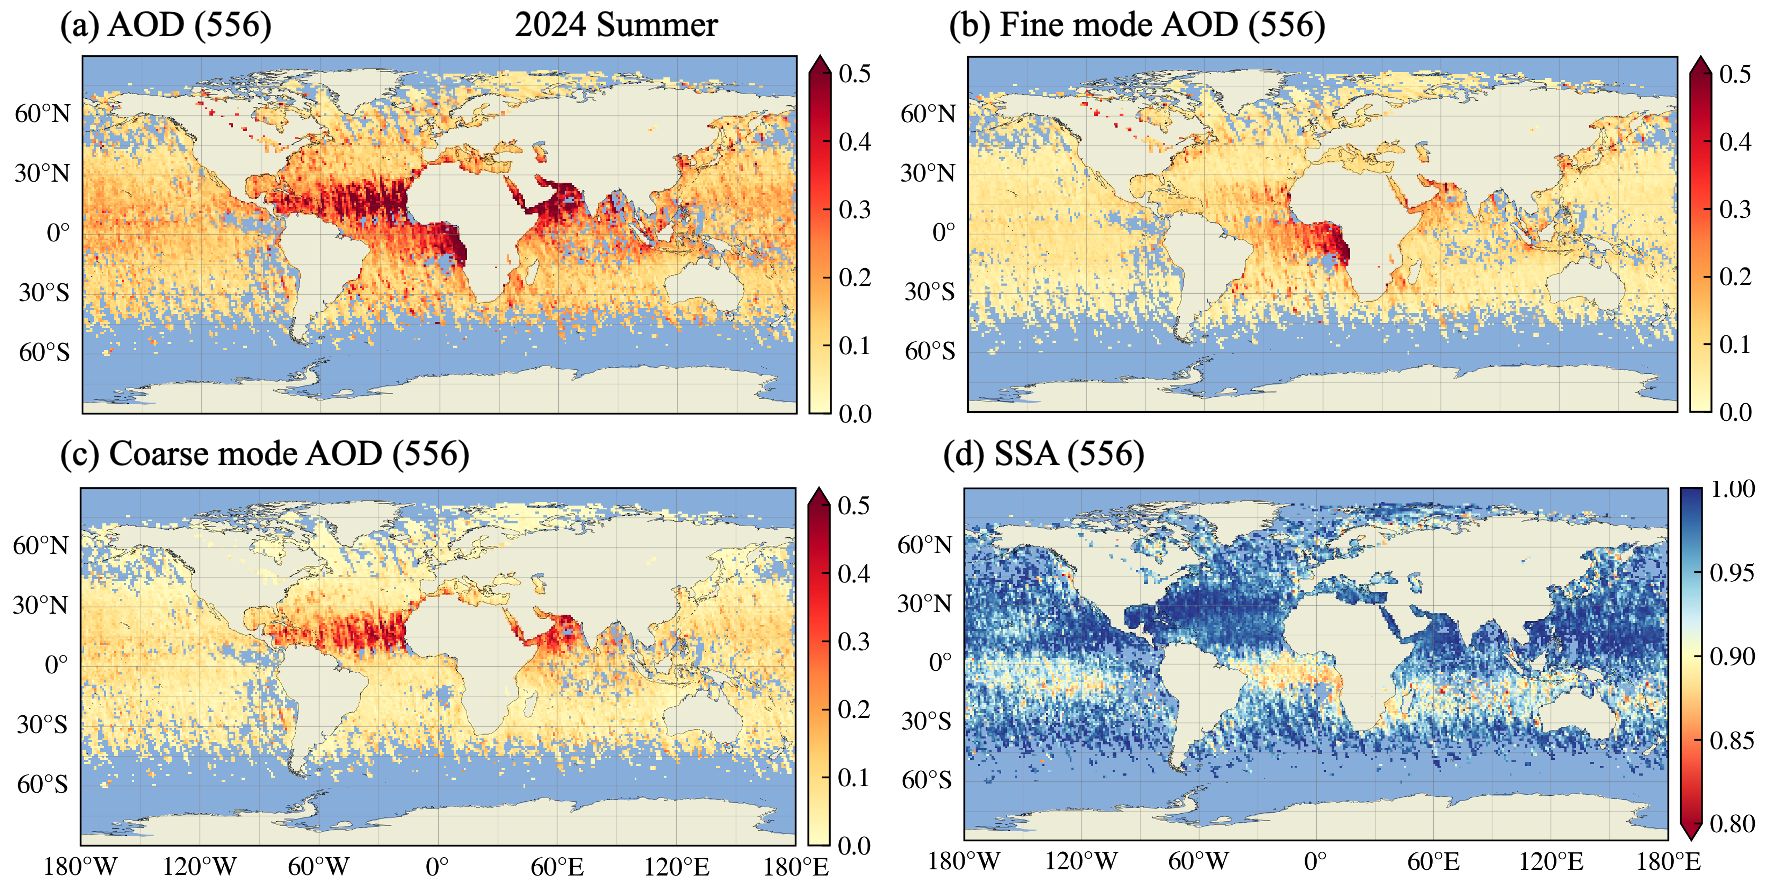
\includegraphics[keepaspectratio]{chapters/../figure/validation_spexone_fig_15_0.04/fig_l3_aerosol_556.png}}

}

\caption{Global aerosol products}

\end{figure}%

\begin{center}\rule{0.5\linewidth}{0.5pt}\end{center}

\textbf{Ocean Products}

Global distributions of \(R_{rs}\) (443, 556, 667 nm) and
chlorophyll-\emph{a}:

\begin{figure}[H]

{\centering \pandocbounded{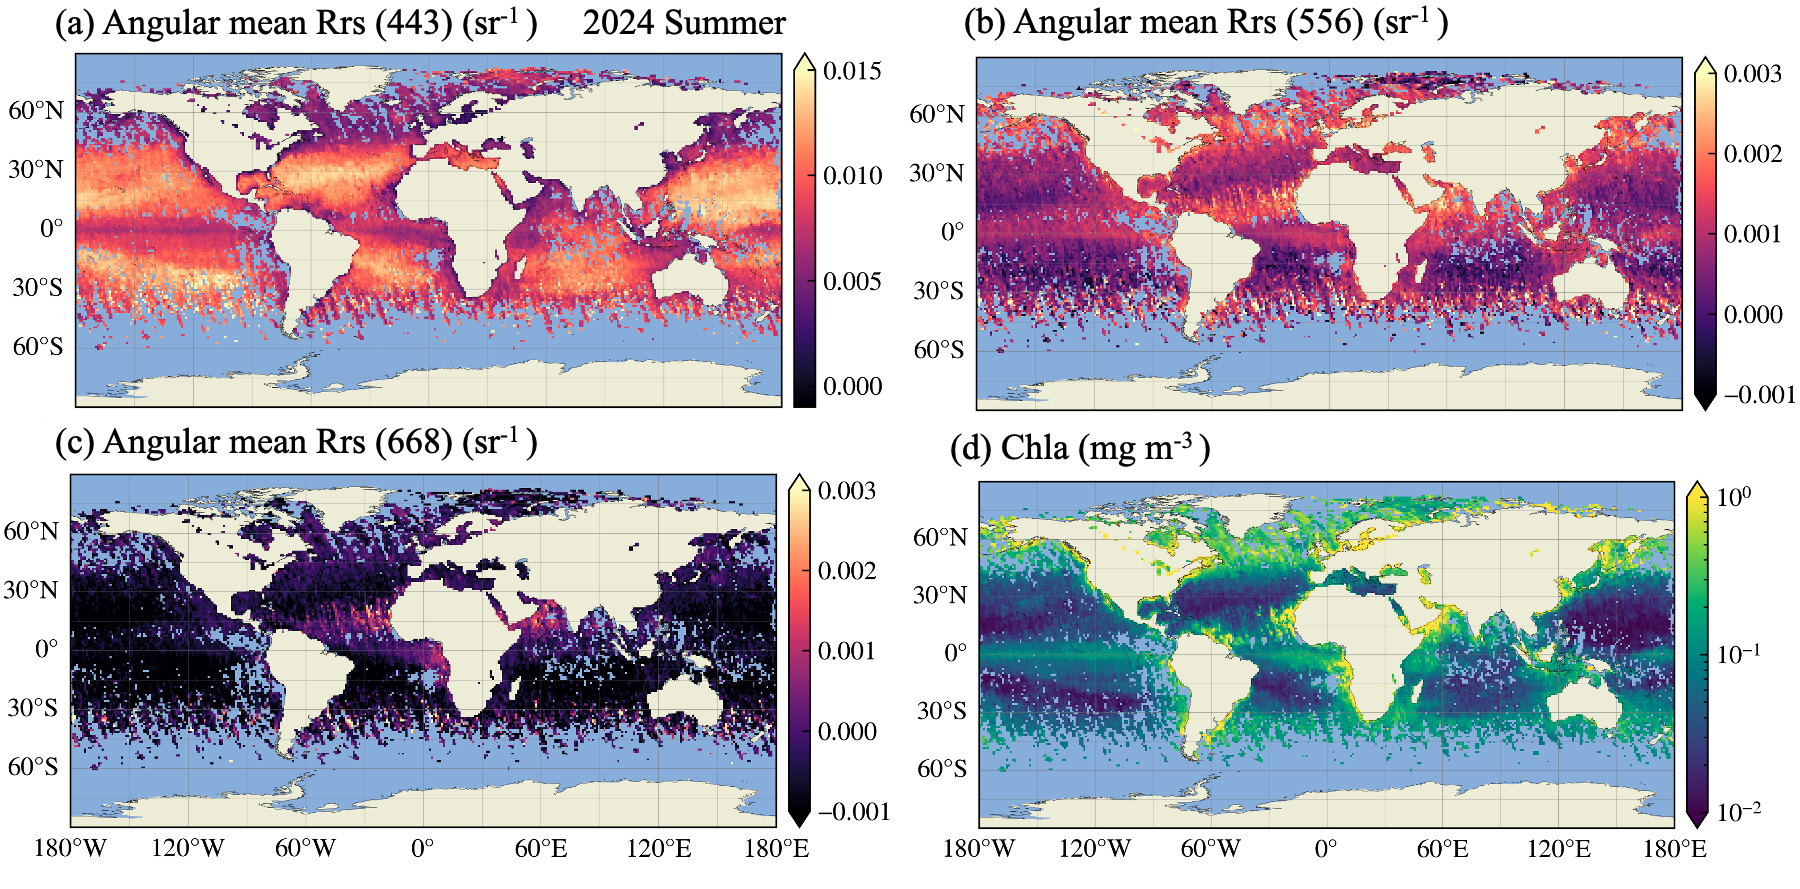
\includegraphics[keepaspectratio]{chapters/../figure/validation_spexone_fig_15_0.04/fig_l3_rrs.png}}

}

\caption{Global ocean products}

\end{figure}%

The retrieved \(R_{rs}\) contains spectral and angular dimensions. The
results shown here represent the BRDF-corrected angular mean.

\textbf{Key result:}\\
The global distributions show realistic spatial and seasonal patterns,
indicating effective separation of atmospheric and oceanic retrieval
components.

\bookmarksetup{startatroot}

\chapter{HARP2 L2 Validation (DITL)}\label{sec-harp2-ditl}

\section{Overview}\label{overview-1}

Pre-launch Day-in-the-Life (DITL) simulations provide an end-to-end
benchmark of HARP2 measurement realism, L2 retrieval performance, and
uncertainty characterization. The results below highlight three key
aspects: synthetic observations, pixel-wise retrieval performance, and
uncertainty analysis. Details are provided in Gao et al.
(\citeproc{ref-Gao:2023aa}{2023}).

Validation of the production data (V3 and V4) is ongoing, following the
methodologies reported in Gao et al. (\citeproc{ref-Gao:2026aa}{2026}).
The validation results should be compared with the DITL uncertainty
analysis to assess retrieval performance using real observations
relative to theoretical expectations.

\section{Summary Information}\label{summary-information-1}

\begin{itemize}
\tightlist
\item
  \textbf{FastMAPOL version:} Prelaunch Test\\
\item
  \textbf{Data period:} March 21, 2022 (spring equinox)\\
\item
  \textbf{Reference:} Synthetic HARP2\\
\item
  \textbf{Published:} Dec 07, 2023
  (https://doi.org/10.5194/amt-16-5863-2023)
\end{itemize}

\section{Synthetic HARP2
observations}\label{synthetic-harp2-observations}

As shown in Figure~\ref{fig-validation_harp2_l1c}, A full day of
synthetic HARP2 observations is generated using a neural network forward
model for both reflectance and DoLP. Aerosol and surface properties are
prescribed from reanalysis (MERRA-2). The simulated observations provide
a realistic testbed for retrieval evaluation:

\begin{itemize}
\tightlist
\item
  Global multi-angle measurements are generated for both reflectance and
  polarization.\\
\item
  DoLP shows enhanced sensitivity to aerosol and surface properties.\\
\item
  Reflectance and DoLP provide complementary information content.
\end{itemize}

\begin{figure}

\centering{

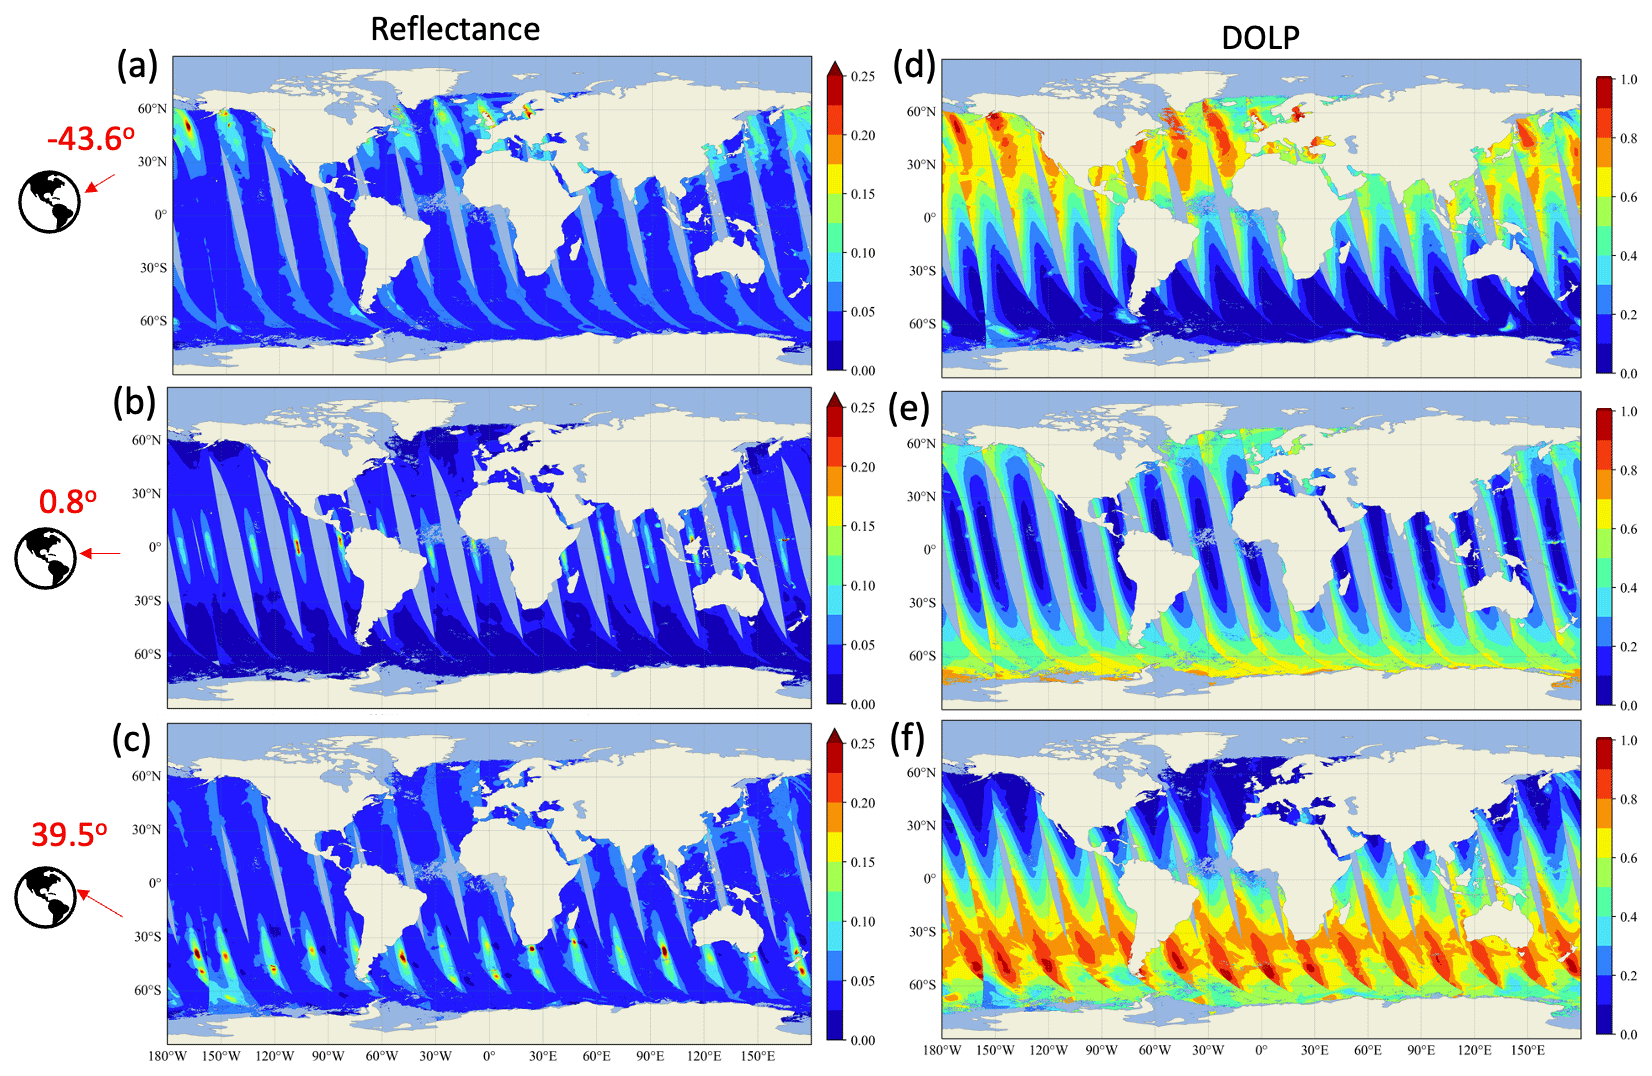
\includegraphics[width=0.8\linewidth,height=\textheight,keepaspectratio]{chapters/../figure/validation_harp2_l1c.png}

}

\caption{\label{fig-validation_harp2_l1c}Global HARP2 simulation (550
nm): reflectance (a--c) and DoLP (d--f) from 15 orbits on 21 March 2022,
showing three along-track viewing angles. Figure is adopted from Gao et
al. (\citeproc{ref-Gao:2023aa}{2023})}

\end{figure}%

\section{Geophysical retrievals with pixel-wise
uncertainty}\label{geophysical-retrievals-with-pixel-wise-uncertainty}

Based on the synthetic data, retrieval results as shown in
Figure~\ref{fig-validation_harp2_l2} demonstrate strong agreement with
truth and meaningful uncertainty estimates:

\begin{itemize}
\tightlist
\item
  AOD (550 nm) is retrieved with high accuracy and low spatial error.\\
\item
  Multiple geophysical variables are retrieved simultaneously, with ALH
  shown as an example.\\
\item
  Pixel-wise uncertainty reflects scene dependence, with larger values
  at low AOD and limited angular sampling.
\end{itemize}

\begin{figure}

\centering{

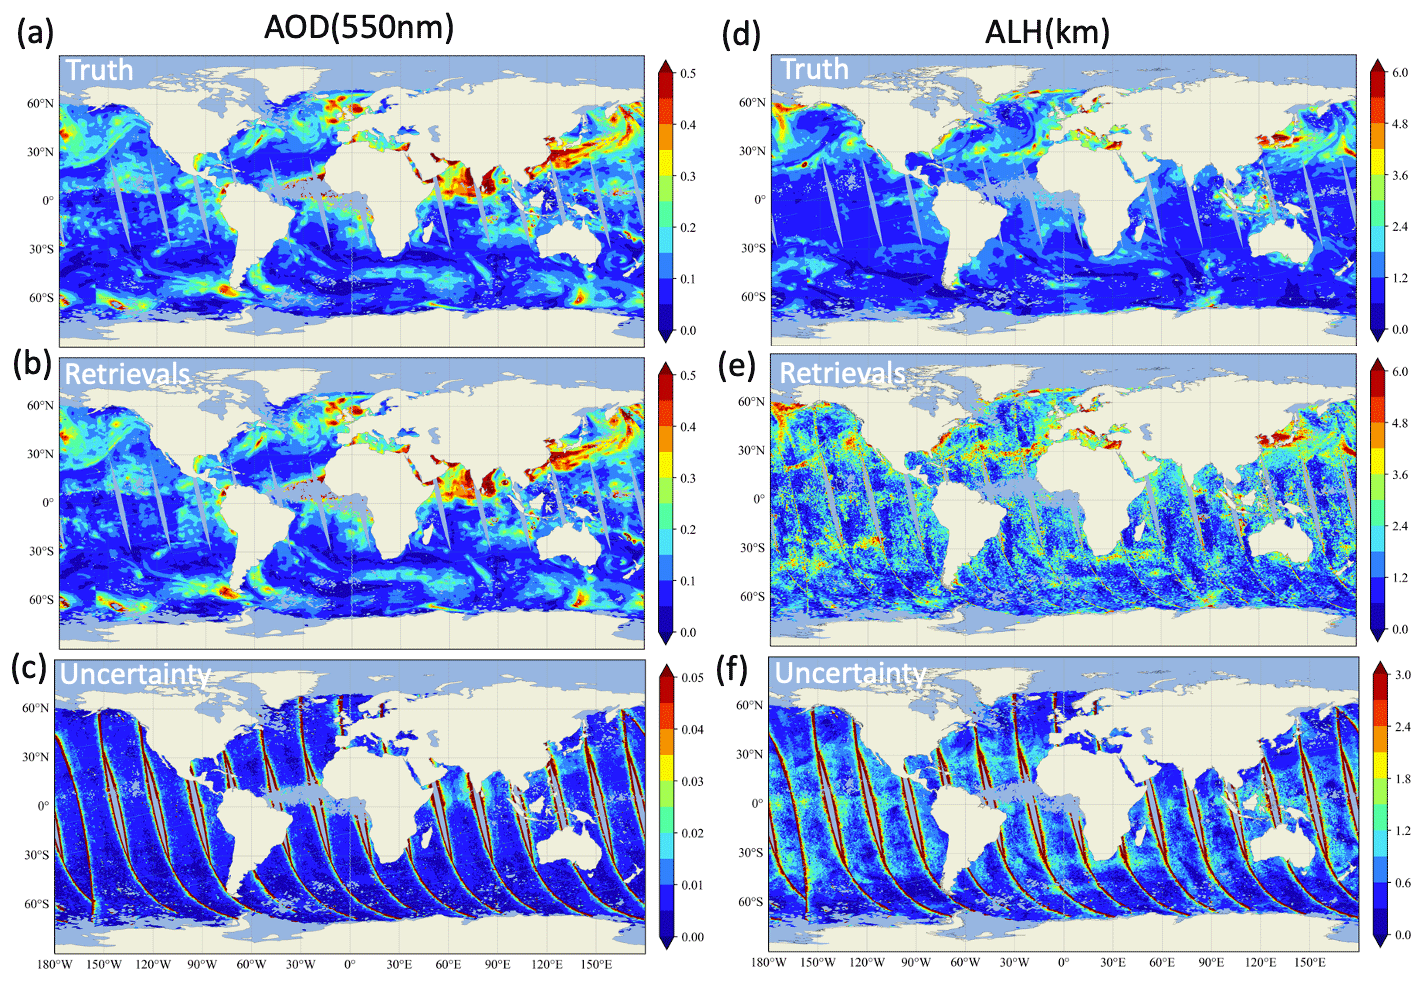
\includegraphics[width=0.8\linewidth,height=\textheight,keepaspectratio]{chapters/../figure/validation_harp2_l2.png}

}

\caption{\label{fig-validation_harp2_l2}Retrieval performance: AOD (550
nm) and ALH showing retrieval, truth, and uncertainty (a--c, d--f).
Figure is adopted from Gao et al. (\citeproc{ref-Gao:2023aa}{2023})}

\end{figure}%

\section{Uncertainty closure
analysis}\label{uncertainty-closure-analysis}

Theoretical uncertainties are derived from error propagation, while
realized uncertainties are computed from retrieval--truth differences.
Their comparisons are shown in Figure~\ref{fig-validation_harp2_unc},

\begin{itemize}
\tightlist
\item
  Good agreement for aerosol optical and microphysical properties,
  especially at moderate to high AOD.\\
\item
  Decreasing uncertainty with increasing aerosol loading.\\
\item
  Underestimation of uncertainty in low-AOD conditions and for weakly
  constrained parameters.
\end{itemize}

\begin{figure}

\centering{

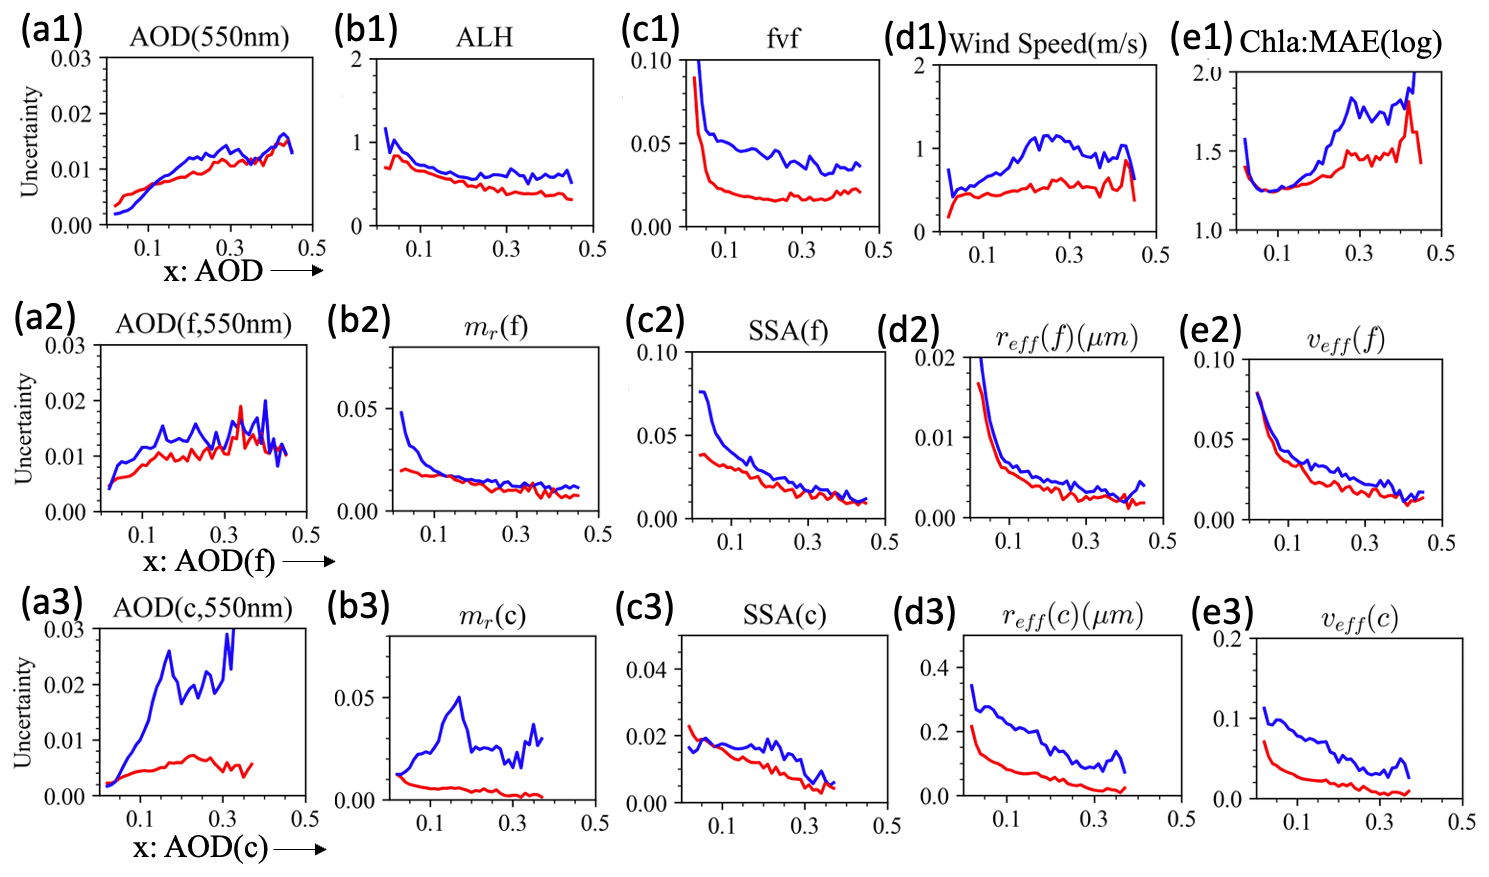
\includegraphics[width=0.9\linewidth,height=\textheight,keepaspectratio]{chapters/../figure/validation_harp2_unc.png}

}

\caption{\label{fig-validation_harp2_unc}Theoretical (red) vs.~retrieved
(blue) uncertainties as a function of AOD for AOD, SSA, mr, reff, veff,
wind speed, and Chl a. AOD ranges from 0.01--0.45 (Δ=0.01). Figure is
adopted from Gao et al. (\citeproc{ref-Gao:2023aa}{2023})}

\end{figure}%

\section{Summary}\label{summary}

\begin{itemize}
\tightlist
\item
  Synthetic data provide realistic multi-angle polarimetric
  observations.\\
\item
  L2 retrievals achieve high accuracy for key variables (especially
  AOD).\\
\item
  Pixel-level uncertainties are physically meaningful and scene
  dependent.\\
\item
  Uncertainty estimates are generally consistent with actual errors,
  with known limitations.
\end{itemize}

These results define a pre-launch benchmark for HARP2 L2 validation
using DITL data.

\bookmarksetup{startatroot}

\chapter{HARP2 L2 Validation (V4)}\label{harp2-l2-validation-v4}

This page summarizes validation results for aerosol and surface products
retrieved from the PACE multi-angle polarimeters using the
\textbf{FastMAPOL} algorithm, with emphasis on \textbf{HARP2} aerosol
optical properties, ocean remote-sensing reflectance (\(R_{rs}\)) and
land surface reflectance (\(\rho_s\)).

FastMAPOL performs coupled aerosol--surface retrievals using an
optimal-estimation framework accelerated by deep neural network forward
models. The validation efforts on HARP2 is ongoing, this page provide
the validation plan following the work by Gao et al.
(\citeproc{ref-Gao:2026aa}{2026}). More results will be updated on the
\href{https://pace.oceansciences.org/pace_fastmapol.htm}{PACE FastMAPOL
validation page}.

\section{Summary Information}\label{summary-information-2}

\begin{itemize}
\tightlist
\item
  \textbf{FastMAPOL version:} v4.0\\
\item
  \textbf{Data period:} 2024/03--2025/12\\
\item
  \textbf{Reference:} AERONET v3, Level 1.5
\end{itemize}

\section{Retrieval Products to be evaluated
(ongoing)}\label{retrieval-products-to-be-evaluated-ongoing}

\textbf{Aerosol} - Total, fine-mode, and coarse-mode aerosol optical
depth (AOD) - Total, fine-mode, and coarse-mode single-scattering albedo
(SSA)

\textbf{Ocean} - Ocean remote-sensing reflectance (\(R_{rs}\))

\textbf{LAND} - Land surface reflectance (\(R_{rs}\)) - \#\# Validation
Strategy

Validation is organized into three levels similar to SPEXone (Gao et al.
(\citeproc{ref-Gao:2026aa}{2026})):

\begin{enumerate}
\def\labelenumi{\arabic{enumi}.}
\item
  \textbf{Global Level-3 assessment}\\
  Evaluate large-scale spatial and seasonal patterns as shown below.
\item
  \textbf{Global aerosol validation}\\
  Compare retrievals with AERONET observations
\item
  \textbf{Joint aerosol--ocean validation}\\
  Evaluate aerosol and \(R_{rs}\) simultaneously using AERONET-OC
  matchups, study the mutual dependencies on the retrieval
  uncertainties.
\end{enumerate}

The objective is to assess both the physical realism of the retrieved
fields and the consistency of aerosol and ocean products.

\section{Global Level-3 Products}\label{global-level-3-products-1}

\textbf{Aerosol Products (556 nm)}

Global distributions of total, fine-mode, and coarse-mode AOD and SSA at
556 nm:

\begin{figure}[H]

{\centering \pandocbounded{\includegraphics[keepaspectratio]{chapters/../figure/fig_harp2_l3_aod.png}}

}

\caption{Global aerosol products}

\end{figure}%

\begin{center}\rule{0.5\linewidth}{0.5pt}\end{center}

\textbf{LAND Products}

Global distributions of \(\rho_{s}\) in RGB (667, 556, 443 nm):

\begin{figure}[H]

{\centering \pandocbounded{\includegraphics[keepaspectratio]{chapters/../figure/fig_harp2_l3_rhos.png}}

}

\caption{Global ocean products}

\end{figure}%

The retrieved \(\rho_s\) contains both spectral and angular dimensions.
The results shown here represent the angular mean after BRDF correction
(\texttt{rhos\_nadir\_mean}).

\textbf{Key result:}\\
The global distributions show realistic spatial and seasonal patterns,
indicating effective separation of atmospheric and surface retrieval
components. Over ocean, AOD shows good consistency with AERONET when
using the best-quality retrievals (quality flags 0 and 1). Over land,
however, retrieved AOD is generally higher than AERONET observations.
For more details, please refer to the Version 4 release notes.

\cleardoublepage
\phantomsection
\addcontentsline{toc}{part}{Appendices}
\appendix

\chapter{Technical Details}\label{technical-details-1}

This section provides detailed mathematical formulations, derivations,
and supporting information for the FastMAPOL algorithm. The material
presented here complements the main chapters and is intended for readers
who require a deeper understanding of the underlying theory,
assumptions, and implementation details.

The appendices include: - Details in radiative transfer model - Details
in the NN and automatic differentation - Detailed formulations of
aerosol size distributions and their moments\\
- Surface reflectance models for ocean and land - Multi-angle
atmospheric correction

These technical details are not required for general use or
interpretation of the FastMAPOL products but are essential for algorithm
development, validation, and advanced scientific analysis.

All equations and formulations follow the conventions introduced in the
main text unless otherwise noted.

Each chapter provides an \textbf{implementation status} indicating where
the described methodology has been applied or its current stage of
development. The status categories include the pre-launch
\textbf{Day-In-The-Life (DITL)} test, with data available through
OB.DAAC; the operational \textbf{PACE V3} and \textbf{PACE V4} products,
available through the Earthdata Cloud; methodologies currently under
\textbf{Evaluation}; and \textbf{Planned} future developments. When
multiple methodological options are available, the Model field
identifies the specific model or configuration to which the
implementation status applies.

For example:

\textbf{Implementation status}

\begin{longtable}[]{@{}lccccc@{}}
\toprule\noalign{}
Model & DITL & PACE V3 & PACE V4 & Evaluation & Planned \\
\midrule\noalign{}
\endhead
\bottomrule\noalign{}
\endlastfoot
--- & x & x & x & --- & --- \\
\end{longtable}

\chapter{Radiative Transfer: PACE Simulator}\label{sec-rt-model}

\textbf{Implementation status}

\begin{longtable}[]{@{}lccccc@{}}
\toprule\noalign{}
Model & DITL & PACE V3 & PACE V4 & Evaluation & Planned \\
\midrule\noalign{}
\endhead
\bottomrule\noalign{}
\endlastfoot
RTSOS Ocean & x & x & x & --- & --- \\
RTSOS Land & - & - & x & --- & --- \\
\end{longtable}

\section{Overview}\label{overview-2}

The physical forward model underlying FastMAPOL is the \textbf{Radiative
Transfer model based on the Successive Order of Scattering (RTSOS)}
method (\citeproc{ref-Zhai:2009aa}{Zhai et al. 2009},
\citeproc{ref-Zhai:2010aa}{2010}). RTSOS is a vector radiative transfer
model developed for coupled atmosphere--ocean and atmosphere-land
systems. For ocean applications, the atmosphere, rough air--sea
interface, and ocean body are treated as a physically coupled system so
that multiple scattering among these components is explicitly included.
For land applications, the atmosphere and land surface are similarly
treated as a physically coupled system, with their interactions
explicitly accounted for.

Key features:

\begin{itemize}
\tightlist
\item
  RTSOS is capable of solving polarized radiative transfer for both
  atmosphere-ocean and atmosphere-land systems.
\item
  In atmosphere-ocean systems, it can also simulate inelastic scattering
  processes, including Raman scattering and fluorescence by chlorophyll
  and colored dissolved organic matter (\citeproc{ref-Zhai:2015aa}{Zhai
  et al. 2015}, \citeproc{ref-Zhai:2017ve}{2017}).
\item
  An improved pseudos-spherical shell (IPSS) algorithm is used to
  improve the simulation of radiance field over polar regions
  (\citeproc{ref-Zhai:2022aa}{Zhai and Hu 2022}).
\end{itemize}

For this work, RTSOS is configured to simulate polarized radiance fields
for randomly generated Earth systems for the PACE instruments
(\citeproc{ref-Zhai:2022bb}{Zhai et al. 2022}). The data are then used
to train neural network forward models, which emulates the behavior of
the radiative transfer system.

\section{The physics of RTSOS}\label{the-physics-of-rtsos}

The model computes the polarized radiation field represented by the
Stokes vector (\citeproc{ref-Zhai:2009aa}{Zhai et al. 2009}),

\[
\mathbf{L}=(I,Q,U,V)^T,
\]

where \(I\) is the total radiance, \(Q\) and \(U\) describe linear
polarization, \(V\) describes circular polarization; the superscript T
stands for vector transpose.

In the RTSOS formulation, the total radiation field is expressed as the
sum of contributions from successive scattering orders,

\[
\mathbf{L} = \sum_{n=0}^{N_s}\mathbf{L}^{(n)} + \mathbf{L}_{\mathrm{geo}},
\]

where \(\mathbf{L}^{(n)}\) represents the contribution from the \(n\)th
order of scattering and \(N_s\) is the maximum scattering order retained
in the numerical calculation. The first-order scattering solution is
evaluated directly, and each subsequent order is obtained by integrating
the radiation field from the preceding order over optical depth and
propagation direction (\citeproc{ref-Zhai:2009aa}{Zhai et al. 2009},
\citeproc{ref-Zhai:2010aa}{2010}). \(\mathbf{L}_{\mathrm{geo}}\) is all
the contributions beyond order \(N_s\), which can be approximated by a
geometric series.

\section{Coupled atmosphere--surface
system}\label{coupled-atmospheresurface-system}

For FastMAPOL ocean retrievals, RTSOS fully accounts for photons which
undergo multiple interactions among atmospheric molecules and aerosols,
the rough ocean surface, and optically active constituents within the
ocean (\citeproc{ref-Zhai:2009aa}{Zhai et al. 2009},
\citeproc{ref-Zhai:2010aa}{2010}, \citeproc{ref-Zhai:2017aa}{2017}).
These developments supported the production of the HARP2 and SPEXone
\texttt{MAPOL\_OCEAN} products. More recent developments have
incorporated a land surface model and have been used to produce the
HARP2 \texttt{MAPOL\_LAND} products.The configuration of atmosphere,
surface, and ocean water body is described below.

\subsection{Atmosphere}\label{atmosphere}

Atmospheric optical properties are specified vertically in terms of
layer optical depth, single-scattering albedo, and scattering phase
matrix. Molecular Rayleigh scattering, gas absorption, aerosol
scattering and absorption are included. RTSOS can also be used to
simulate cloud radiative transfer, which is however not used in
FastMAPOL.

The molecular atmosphere is characterized using vertical profiles of the
total atmospheric molecular number density and the mixing ratios of
absorbing gases. Gas absorption from major species relevant to the PACE
spectral range, including \(H_2O\), \(CO_2\), \(O_2\), \(CH_4\),
\(O_3\), and \(NO_2\), are included. In the PACE simulator,
high-resolution absorption cross sections for several gases are
generated using molecular spectroscopic information from HITRAN
(\citeproc{ref-Gordon:2022aa}{Gordon et al. 2022}), with dedicated ozone
and NO\(_2\) datasets used where appropriate
(\citeproc{ref-Burrows:1998aa}{Burrows et al. 1998};
\citeproc{ref-Serdyuchenko:2014aa}{Serdyuchenko et al. 2014};
\citeproc{ref-Zhai:2022bb}{Zhai et al. 2022}).

Aerosol single-scattering properties, including extinction coefficients,
single scattering albedos, and Mueller scattering matrices are supplied
to RTSOS. The radiative transfer solver itself is therefore not
restricted to a particular aerosol particle model. Optical properties
obtained from Mie calculations, T-matrix methods, discrete-dipole
calculations, or other electromagnetic scattering models can be used as
inputs. This flexibility is important for FastMAPOL, where aerosol
properties are parameterized differently in different generations of the
retrieval algorithm.

RTSOS supports flexible aerosol models, with further details on those
used in FastMAPOL provided in Appendix~\ref{sec-aerosol-model}.

\subsection{Air--sea interface}\label{airsea-interface}

The air--sea interface is represented as a wind-roughened surface.
Reflection and transmission of polarized radiation across the interface
are treated using reflection and transmission matrices, including
repeated interactions between the atmosphere, ocean surface, and water
body (\citeproc{ref-Zhai:2010aa}{Zhai et al. 2010}).

Surface roughness is parameterized primarily through wind speed using a
Cox--Munk wave-slope distribution (\citeproc{ref-Cox:1954aa}{Cox and
Munk 1954}). Consequently, RTSOS explicitly represents the angular
structure of ocean glint rather than masking the glint region by
default. In early versions of FastMAPOL, the NN training excluded the
sunglint region to prevent the large reflectance values near glint from
degrading NN accuracy at non-glint viewing angles, as implemented in the
AirHARP study (\citeproc{ref-Gao:2021aa}{Gao et al. 2021}). More recent
versions of FastMAPOL accurately represent RTSOS simulations across the
full range of viewing angles, including the sunglint region, through
uncertainty-aware NN training, as implemented for the Version 3 and
Version 4 products (\citeproc{ref-Gao:2023aa}{Gao et al. 2023};
\citeproc{ref-Gao:2026aa}{Gao et al. 2026}). Retaining the sunglint
region provides useful retrieval information, particularly for surface
wind speed and absorbing aerosols for
HARP2(\citeproc{ref-Gao:2023aa}{Gao et al. 2023}) and more HARP2 and
SPEXone combined (\citeproc{ref-Aryal:2024aa}{Aryal et al. 2024}).

Foam and whitecap fraction on rough ocean surface and their reflectance
are parameterized in terms of wind speed following
(\citeproc{ref-Koepke:1984aa}{Koepke 1984}) in the FastMAPOL simulation
configuration.

\subsection{Ocean body}\label{ocean-body}

The ocean inherent optical properties include contributions from pure
seawater, phytoplankton, non-algal particles, and colored dissolved and
detrital material. Particle scattering is represented through the
Fournier-Forand phase function (\citeproc{ref-Fournier:1994aa}{Fournier
and Forand 1994}) and the average Mueller matrix measured
(\citeproc{ref-Voss:1984aa}{Voss and Fry 1984}), while absorption and
scattering coefficients are parameterized through retrievable
bio-optical quantities.

Three parameterization approaches for the bio-optical models have been
evaluated, as discussed in Appendix~\ref{sec-ocean-model}, with varying
levels of complexity.

For the single-parameter model used in Version 3 and Version 4 data
production (\citeproc{ref-Gao:2023aa}{Gao et al. 2023};
\citeproc{ref-Gao:2026aa}{Gao et al. 2026}), the absorption and
scattering properties of ocean water are parameterized in terms of
chlorophyll-a concentration, providing computational efficiency while
maintaining retrieval accuracy.

For more complex waters, the absorption and scattering coefficients are
parameterized using retrievable bio-optical quantities
(\citeproc{ref-Aryal:2024aa}{Aryal et al. 2024},
\citeproc{ref-Aryal:2026aa}{2026}). This expanded representation allows
the radiative transfer training database to encompass waters in which
inherent optical properties (IOPs) do not covary uniquely with
chlorophyll-a concentration. This approach, also called
FastMAPOL/componnet, is planned for future FastMAPOL data production
over coastal waters.

\subsection{Land Surface}\label{land-surface}

RTSOS also performs coupled atmosphere--land surface simulations. The
land surface is represented using the Ross--Li model, as described in
Appendix~\ref{sec-land-model}, with the corresponding data products
discussed in Chapter~\ref{sec-data-format}.

\section{Numerical treatment}\label{numerical-treatment}

RTSOS discretizes the zenith-angle dependence of the radiation field
using Gaussian quadrature and represents azimuthal dependence using a
Fourier expansion. Strongly forward-peaked aerosol and hydrosol
scattering functions can otherwise require a large number of angular
quadrature points. RTSOS therefore includes phase-function truncation
techniques, including the \(\delta\)-M
(\citeproc{ref-Wiscombe:1977aa}{Wiscombe 1977}), \(\delta\)-fit
(\citeproc{ref-Hu:2000aa}{Hu et al. 2000}), and related approaches, to
improve computational efficiency while preserving radiometric accuracy
(\citeproc{ref-Zhai:2009aa}{Zhai et al. 2009},
\citeproc{ref-Zhai:2022bb}{2022}).

For geometries with large solar or viewing zenith angles, the
plane-parallel approximation becomes less accurate because of the
curvature of the atmosphere. RTSOS therefore incorporates an
\textbf{improved pseudo-spherical shell (IPSS)} correction
(\citeproc{ref-Zhai:2022aa}{Zhai and Hu 2022}). The IPSS treatment
calculates the exact single scattering solution with spherical geometry
while using the computationally efficient plane-parallel
multiple-scattering solution to estimate the higher-order contribution.
This substantially improves accuracy at large zenith angles and is
particularly relevant to high-latitude observations. Additional details
are provided in Appendix~\ref{sec-rt-shell}.

\section{PACE instrument simulator}\label{pace-instrument-simulator}

RTSOS forms the monochromatic radiative transfer core of a more general
PACE simulator developed to reproduce the measurements of the three PACE
instruments: OCI, HARP2, and SPEXone (\citeproc{ref-Zhai:2022bb}{Zhai et
al. 2022}). The simulator couples the wavelength-dependent atmosphere
and ocean optical properties with instrument spectral and viewing
characteristics to generate synthetic TOA observations.

The full PACE simulator supports hyperspectral radiance simulations for
OCI and multi-angle polarized radiance simulations for HARP2 and
SPEXone. Instrument spectral response is important near strong molecular
absorption bands, where using only the absorption coefficient at the
nominal center wavelength can introduce substantial radiance errors. The
PACE simulator therefore includes spectral integration procedures for
resolving gas absorption within instrument bands
(\citeproc{ref-Zhai:2022bb}{Zhai et al. 2022}).

FastMAPOL does not necessarily use every wavelength available from the
instruments. Instead, instrument-dependent wavelength subsets are
selected to balance information content and computational cost. The
wavelength configuration may change between algorithm versions. For
example, four spectral bands are used for HARP2, whereas 34 spectral
bands are used for SPEXone in both V3 and V4 data
(Chapter~\ref{sec-data-format}). The FastMAPOL/component version
implementation combines measurements from both HARP2 and SPEXone and
uses a total of 13 wavelengths (\citeproc{ref-Aryal:2024aa}{Aryal et al.
2024}) (Appendix~\ref{sec-aerosol-component}).

\section{Radiometric quantities generated for
FastMAPOL}\label{radiometric-quantities-generated-for-fastmapol}

RTSOS can calculate the complete Stokes vector at the TOA, within the
atmosphere, immediately above or below the ocean surface, and at
specified depths within the ocean (\citeproc{ref-Zhai:2009aa}{Zhai et
al. 2009}, \citeproc{ref-Zhai:2022bb}{2022}). FastMAPOL primarily uses
several derived quantities from these simulations.

The TOA reflectance is defined as

\[
\rho_t =
\frac{\pi I_t}{\mu_0 F_0},
\]

where \(I_t\) is the TOA radiance, \(\mu_0\) is the cosine of the solar
zenith angle, and \(F_0\) is the extraterrestrial solar irradiance.

The degree of linear polarization is

\[
P_t =
\frac{\sqrt{Q_t^2+U_t^2}}{I_t}.
\]

\section{Atmospheric Correction and Ocean
Color}\label{atmospheric-correction-and-ocean-color}

In addition to the total TOA signal, RTSOS can perform simulations with
the ocean-body contribution removed. This produces the reflectance
associated with the atmosphere and ocean surface,
\(\rho^{f}_{t,\mathrm{atm+sfc}}\). The water-leaving contribution
reaching the sensor can therefore be obtained from

\[
\rho_w = \rho_t-\rho^{f}_{t,\mathrm{atm+sfc}}
\]

This ability to explicitly label and separate photon contributions is a
useful property of the RTSOS formulation
(\citeproc{ref-Zhai:2009aa}{Zhai et al. 2009},
\citeproc{ref-Zhai:2017aa}{2017}) and provides a physically consistent
method for atmospheric correction. This approach has been implemented
with the additional use of NNs to produce FastMAPOL ocean color products
(\citeproc{ref-Aryal:2024aa}{Aryal et al. 2024};
\citeproc{ref-Gao:2021aa}{Gao et al. 2021};
\citeproc{ref-Gao:2026aa}{Gao et al. 2026}).

FastMAPOL also uses RTSOS to calculate quantities required for
bidirectional reflectance correction. Rather than relying exclusively on
an empirical BRDF correction, simulations can be performed for the
retrieved atmosphere--ocean system at both the actual observation
geometry and a reference geometry (Appendix~\ref{sec-ocean-ac}). This
permits the angular dependence of the water-leaving radiance to be
derived consistently from the same radiative transfer physics used in
the retrieval (\citeproc{ref-Gao:2026aa}{Gao et al. 2026}). The
corresponding products are discussed in Chapter~\ref{sec-data-format}.

\section{Additional RTSOS
capabilities}\label{additional-rtsos-capabilities}

RTSOS contains capabilities that extend beyond those required by the
current elastic-scattering FastMAPOL retrieval. In ocean waters, the
model can solve the inelastic vector radiative transfer equation and
simulate Raman scattering by water as well as fluorescence by
phytoplankton and dissolved organic matter
(\citeproc{ref-Zhai:2015aa}{Zhai et al. 2015},
\citeproc{ref-Zhai:2017ve}{2017}, \citeproc{ref-Zhai:2018hc}{2018}).
These processes couple radiation at different excitation and emission
wavelengths and are evaluated using the elastic RTSOS radiation field to
construct the corresponding inelastic source terms.

These capabilities are useful for hyperspectral ocean-color studies and
future extensions of FastMAPOL, but they should be distinguished from
the elastic radiative transfer simulations currently used to generate
the primary FastMAPOL neural-network training datasets.

\section{Model heritage and application to
FastMAPOL}\label{model-heritage-and-application-to-fastmapol}

RTSOS has evolved from the original coupled atmosphere--ocean model with
a flat ocean surface (\citeproc{ref-Zhai:2009aa}{Zhai et al. 2009}) to
the treatment of a rough ocean interface
(\citeproc{ref-Zhai:2010aa}{Zhai et al. 2010}), from elastic scattering
only to inelastic ocean processes (\citeproc{ref-Zhai:2015aa}{Zhai et
al. 2015}, \citeproc{ref-Zhai:2017ve}{2017}), from plane-parallel to
improved spherical-shell geometry (\citeproc{ref-Zhai:2022aa}{Zhai and
Hu 2022}), and monochromatic simulation to the complete PACE instrument
simulator (\citeproc{ref-Zhai:2022bb}{Zhai et al. 2022}).

Within FastMAPOL, RTSOS provides the high-fidelity physical reference
from which the neural-network forward models are constructed. The
resulting framework therefore combines a rigorous coupled
atmosphere--ocean and atmosphere--land vector radiative transfer model
with computationally efficient machine-learning emulators, enabling
simultaneous aerosol, ocean-color, and surface retrievals from PACE
multi-angle polarimetric observations (\citeproc{ref-Aryal:2024aa}{Aryal
et al. 2024}, \citeproc{ref-Aryal:2026aa}{2026};
\citeproc{ref-Gao:2023aa}{Gao et al. 2023};
\citeproc{ref-Gao:2026aa}{Gao et al. 2026}).

\textbf{Code availability.} The RTSOS code is maintained and developed
by Pengwang Zhai. The source code and example configurations are
publicly available through the
\href{https://github.com/aoog-umbc/rtsos-public}{AOOG/UMBC RTSOS
repository}. For additional information, please contact Pengwang Zhai
(\href{mailto:pwzhai@umbc.edu}{\nolinkurl{pwzhai@umbc.edu}}).

\chapter{Radiative Transfer: Spherical Shell
Correction}\label{sec-rt-shell}

\textbf{Implementation status}

\begin{longtable}[]{@{}lccccc@{}}
\toprule\noalign{}
Model & DITL & PACE V3 & PACE V4 & Evaluation & Planned \\
\midrule\noalign{}
\endhead
\bottomrule\noalign{}
\endlastfoot
--- & x & x & x & --- & --- \\
\end{longtable}

As discussed in Appendix~\ref{sec-rt-model} and Gao et al.
(\citeproc{ref-Gao:2023aa}{2023}), the FastMAPOL forward-model training
data are generated using a PACE-tailored vector radiative transfer model
based on the successive orders of scattering method
(\citeproc{ref-Zhai:2022bb}{Zhai et al. 2022}). An improved
pseudo-spherical shell (IPSS) correction is applied to account for Earth
curvature and improve radiative transfer accuracy, particularly at large
solar and viewing zenith angles (\citeproc{ref-Zhai:2022aa}{Zhai and Hu
2022}).

Reflectance and degree of linear polarization (DoLP) are simulated at
the PACE satellite altitude of approximately 676 km above Earth's
surface. Because of Earth curvature, the solar and viewing zenith angles
at the satellite altitude differ from those defined at the Earth's
surface, as illustrated in Figure~\ref{fig-system}. The IPSS treatment
accounts for this geometric difference when performing the radiative
transfer calculations.

\begin{figure}

\centering{

\includegraphics[width=10cm,height=\textheight,keepaspectratio]{chapters/../figure/fig_rt_shell.png}

}

\caption{\label{fig-system}Spherical-shell geometry and transformation
between satellite and surface viewing geometries.}

\end{figure}%

In FastMAPOL, the solar and viewing geometries used as inputs to the NN
forward models are defined at the Earth's surface, consistent with the
geometry convention used in the PACE Level-1C (L1C) products. Thus, all
FastMAPOL forward-model inputs and PACE L1C observations use the same
geometric reference convention.

In Figure~\ref{fig-system}, \(\theta'_0\) and \(\theta'_v\) denote the
solar and viewing zenith angles defined at the satellite altitude, while
\(\theta_0\) and \(\theta_v\) denote the corresponding angles at the
Earth's surface. The transformations between these geometries follow
Zhai and Hu (\citeproc{ref-Zhai:2022aa}{2022}). The solar and viewing
azimuth angles are treated consistently within the corresponding
reference frames but are not shown in the figure.

This treatment allows the radiative transfer calculations to account for
the spherical-shell geometry of the Earth--atmosphere system while
maintaining surface-referenced geometry as the common interface between
the PACE L1C measurements and the FastMAPOL NN forward models.

\chapter{Retrieval: Inversion Algorithm}\label{sec-retrieval-inversion}

FastMAPOL formulates the retrieval as a constrained nonlinear
least-squares optimization problem. The cost function is defined in
Chapter~\ref{sec-retrieval} and is restated here for completeness:

\[
\chi^2({\mathbf x})
=
\frac{1}{N}
\sum_i
\left[
\frac{[\rho_t(i)-\rho_t^f({\mathbf x};i)]^2}{\sigma_\rho^2(i)}
+
\frac{[P_t(i)-P_t^f({\mathbf x};i)]^2}{\sigma_P^2(i)}
\right].
\]

Here, \(\rho_t^f\) and \(P_t^f\) are the NN forward-model predictions of
reflectance and DoLP, respectively. The state vector \(\mathbf{x}\)
contains the aerosol and surface parameters for the selected FastMAPOL
retrieval configuration, with each parameter constrained to a physically
meaningful range.

The cost function can equivalently be written in matrix form as

\begin{equation}\phantomsection\label{eq-uq-cost}{
\chi^2
=
\frac{1}{N}
\left[
\mathbf{F}(\mathbf{x})-\mathbf{m}
\right]^T
\mathbf{S}_{\epsilon}^{-1}
\left[
\mathbf{F}(\mathbf{x})-\mathbf{m}
\right],
}\end{equation}

where \(\mathbf{m}\) is the measurement vector containing reflectance
and DoLP observations from the available wavelengths and viewing angles,
\(\mathbf{F}(\mathbf{x})\) is the corresponding forward-model
calculation, \(N\) is the total number of measurements, and
\(\mathbf{S}_{\epsilon}\) is the measurement and forward-model error
covariance matrix.

\section{Measurement and Forward-Model
Uncertainties}\label{measurement-and-forward-model-uncertainties}

The uncertainties used to weight the cost function account for
contributions from the instrument, NN forward-model approximation, and
numerical accuracy of the radiative transfer (RT) simulations used to
generate the NN training data. For reflectance and DoLP, respectively,

\begin{equation}\phantomsection\label{eq-sigma-rho}{
\sigma_\rho^2
=
\sigma_{\rho,\mathrm{ins}}^2
+
\sigma_{\rho,\mathrm{NN}}^2
+
\sigma_{\rho,\mathrm{RT}}^2,
}\end{equation}

and

\begin{equation}\phantomsection\label{eq-sigma-P}{
\sigma_P^2
=
\sigma_{P,\mathrm{ins}}^2
+
\sigma_{P,\mathrm{NN}}^2
+
\sigma_{P,\mathrm{RT}}^2.
}\end{equation}

Here, \(\sigma_{\mathrm{ins}}\) represents the instrument measurement
uncertainty, \(\sigma_{\mathrm{NN}}\) represents the uncertainty
introduced by the NN approximation of the forward model, and
\(\sigma_{\mathrm{RT}}\) represents the numerical uncertainty of the RT
calculations. More discussions on the instrument uncertainties are
provided in Appendix~\ref{sec-retrieval-unc-model}.

The NN forward-model uncertainties are determined during NN training and
evaluation (\citeproc{ref-Gao:2021aa}{Gao et al. 2021},
\citeproc{ref-Gao:2023aa}{2023}), with the current NN architectures and
associated uncertainties summarized in Table~\ref{tbl-nn-arch}. In the
current implementation, the uncertainties are assumed to be spectrally
and angularly uncorrelated, such that \(\mathbf{S}_{\epsilon}\) is
diagonal.

\section{Nonlinear Least-Squares
Optimization}\label{nonlinear-least-squares-optimization}

As discussed in Gao et al. (\citeproc{ref-Gao:2021aa}{2021}), to
minimize the cost function, FastMAPOL uses the \textbf{Subspace
Trust-Region Interior Reflective (STIR)} method
(\citeproc{ref-Branch:1999aa}{Branch et al. 1999}), implemented as the
\textbf{Trust Region Reflective (TRF)} nonlinear least-squares algorithm
in the Python SciPy package (\citeproc{ref-SciPy:2020aa}{Virtanen et al.
2020}). The method iteratively solves for the state vector
\(\mathbf{x}\) while enforcing prescribed lower and upper bounds on the
retrieved parameters.

STIR belongs to the family of trust-region least-squares methods and is
closely related to the Levenberg--Marquardt approach
(\citeproc{ref-More:1978aa}{Moré 1978}), while extending the
optimization to efficiently handle bound-constrained problems. The
method provides good numerical stability near parameter boundaries,
which is particularly important for FastMAPOL because many aerosol and
surface parameters are restricted to physically meaningful or
model-defined ranges.

The name \textbf{STIR} summarizes several key features of the
optimization:

\begin{itemize}
\tightlist
\item
  \textbf{Subspace (S):} the optimization step can be determined within
  a reduced-dimensional subspace, improving computational efficiency for
  large optimization problems.
\item
  \textbf{Trust Region (T):} the nonlinear cost function is locally
  approximated using the residuals and Jacobian, and the state-vector
  update is restricted to a region where this local approximation is
  considered reliable.
\item
  \textbf{Interior (I):} the optimization maintains the state parameters
  within their prescribed bounds and uses their distances from the
  bounds in scaling the optimization problem.
\item
  \textbf{Reflective (R):} reflected search directions are considered
  near parameter boundaries, allowing the optimization to continue
  efficiently within the feasible parameter space.
\end{itemize}

At each FastMAPOL iteration, the NN forward model calculates the
simulated measurements and residuals for the current state vector. The
Jacobian matrix,

\begin{equation}\phantomsection\label{eq-retrieval-jacobian}{
K_{ij}
=
\frac{\partial F_i}{\partial x_j},
}\end{equation}

provides the sensitivity of each modeled measurement \(F_i\) to each
retrieved state parameter \(x_j\).

The forward operation of the NN is defined in
Appendix~\ref{sec-nn-model}. During the forward pass, the intermediate
values at each NN layer are stored and subsequently used to calculate
the Jacobian through either forward-mode automatic differentiation
(Table~\ref{tbl-ad-forward}) or reverse-mode automatic differentiation
(backpropagation; Table~\ref{tbl-ad-reverse}).

The residuals and Jacobian are supplied to the TRF optimizer to
determine the next update of the state vector. This process is repeated
until the convergence criteria are satisfied or the maximum number of
iterations is reached.

\section{Convergence}\label{convergence}

FastMAPOL uses three convergence criteria in the TRF optimization, with
a tolerance of 0.01 applied to each:

\begin{itemize}
\tightlist
\item
  \texttt{ftol\ =\ 0.01}, based on the change in the cost function;
\item
  \texttt{xtol\ =\ 0.01}, based on the change in the state vector; and
\item
  \texttt{gtol\ =\ 0.01}, based on the optimality condition determined
  from the cost-function gradient.
\end{itemize}

The optimization terminates when the corresponding SciPy TRF convergence
criterion is satisfied. The resulting state vector provides the
retrieved aerosol and surface properties for the pixel.

Following convergence, the retrieval is evaluated using the adaptive
multi-angle data-screening procedure described in
Appendix~\ref{sec-data-screening}. If one or more measurements are
excluded by the screening criteria, the inversion is repeated using the
previous solution as the initial state. This screening and re-retrieval
process continues until the screening criteria are satisfied or the
maximum number of screening passes is reached.

\section{Interpretation of the Cost
Function}\label{interpretation-of-the-cost-function}

The final cost function provides an overall measure of agreement between
the observations and forward model relative to the assumed
uncertainties. For an ensemble of retrievals, the distribution of the
normalized cost function can be compared with the theoretical \(\chi^2\)
distribution (\citeproc{ref-Gao:2021bb}{Gao et al. 2021}):

\begin{equation}\phantomsection\label{eq-chi2-pdf}{
f(\chi^2,k)
=
\frac{
(\chi^2)^{k/2-1}
k^{k/2}
\exp(-k\chi^2/2)
}{
2^{k/2}\Gamma(k/2)
}.
}\end{equation}

Here, \(k\) represents the number of degrees of freedom (DOF). When
correlations among measurement uncertainties and the effects of
retrieved parameters are neglected, the DOF can be approximated from the
number of measurements. More generally, the effective DOF depends on the
information content of the measurements and retrieved state parameters
and can be evaluated using the Jacobian and error covariance matrices
(\citeproc{ref-Gao:2021bb}{Gao et al. 2021},
\citeproc{ref-Gao:2026aa}{2026}; \citeproc{ref-Gao:2023bb}{Gao et al.
2023}).

\chapter{Retrieval: Input Uncertainty
Model}\label{sec-retrieval-unc-model}

\textbf{Implementation status}

\begin{longtable}[]{@{}lccccc@{}}
\toprule\noalign{}
Model & DITL & PACE V3 & PACE V4 & Evaluation & Planned \\
\midrule\noalign{}
\endhead
\bottomrule\noalign{}
\endlastfoot
HARP2 & x & x & x & --- & --- \\
SPEXone & --- & x & x & --- & --- \\
\end{longtable}

As discussed in Chapter~\ref{sec-retrieval} and later in Appendix
Appendix~\ref{sec-retrieval-inversion}, measurement uncertainties are
used to weight the observations in the retrieval cost function. The
uncertainty model accounts for contributions from instrument measurement
uncertainty, NN forward-model approximation, and numerical uncertainty
in the radiative transfer (RT) simulations used to generate the NN
training dataset.

The RT and NN contributions are evaluated based on factors such as the
RT model configuration, the number of Gaussian quadrature points and
scattering orders, and the size and performance of the NN training
dataset (\citeproc{ref-Gao:2021aa}{Gao et al. 2021}).

Instrument measurement uncertainties depend on the characteristics and
calibration performance of each instrument and are based on information
provided by the instrument teams. For the current FastMAPOL retrievals
used in all the previous versions and studies {[}Gao et al.
(\citeproc{ref-Gao:2021aa}{2021}); Gao:2023aa; Gao et al.
(\citeproc{ref-Gao:2026aa}{2026}){]}, the following measurement
uncertainties are adopted:

\begin{longtable}[]{@{}lrr@{}}
\toprule\noalign{}
Instrument & Reflectance uncertainty & DoLP uncertainty \\
\midrule\noalign{}
\endhead
\bottomrule\noalign{}
\endlastfoot
HARP2 & 3\% & 0.005 \\
SPEXone & 2\% & 0.003 \\
\end{longtable}

The reflectance uncertainty is specified as a relative uncertainty,
whereas the DoLP uncertainty is specified as an absolute uncertainty.
These values are used in constructing the measurement uncertainty terms
that weight the corresponding observations in the retrieval cost
function.

Note that above table denotes the current instrument uncertainty model
used in the retrievals. These uncertainty models may be updated in the
future to reflect changes in instrument characterization or calibration
provided by the instrument teams.

\chapter{Retrieval: Adaptive Multi-angle Data
Screening}\label{sec-data-screening}

\textbf{Implementation status}

\begin{longtable}[]{@{}lccccc@{}}
\toprule\noalign{}
Model & DITL & PACE V3 & PACE V4 & Evaluation & Planned \\
\midrule\noalign{}
\endhead
\bottomrule\noalign{}
\endlastfoot
--- & x & x & x & --- & --- \\
\end{longtable}

FastMAPOL implements an adaptive multi-angle data screening approach to
identify and remove individual observations that cannot be adequately
represented by the forward model, while retaining valid measurements
from the same pixel. This approach is particularly useful for
multi-angle polarimetric observations, where clouds, sunglint, surface
heterogeneity, or other scene-dependent effects may affect only a subset
of viewing angles. The overall retrieval and screening workflow is
illustrated in Figure~\ref{fig-flowchart-screening}, with additional
details and applications provided in Gao et al.
(\citeproc{ref-Gao:2021bb}{2021}).

\begin{figure}

\centering{

\includegraphics[width=0.8\linewidth,height=\textheight,keepaspectratio]{chapters/../figure/fig_data_screening.png}

}

\caption{\label{fig-flowchart-screening}FastMAPOL retrieval workflow (A)
and adaptive multi-angle polarimetric data screening (MAPDS) procedure
(B). Adapted from Gao et al. (\citeproc{ref-Gao:2021bb}{2021}).}

\end{figure}%

\section{Screening Criteria}\label{screening-criteria}

After each converged FastMAPOL retrieval, the residuals between the
measurements and forward-model predictions are evaluated for each
viewing angle. For reflectance and DoLP, the screening criteria are

\begin{equation}\phantomsection\label{eq-data-screening}{
\frac{|\Delta\rho_t|}{\sigma_\rho} < \xi,
\qquad
\frac{|\Delta P_t|}{\sigma_P} < \xi,
}\end{equation}

where \(\Delta\rho_t\) and \(\Delta P_t\) are the differences between
the measurements and forward-model predictions, \(\sigma_\rho\) and
\(\sigma_P\) are the corresponding uncertainties defined in the
retrieval cost function, and \(\xi\) is the screening threshold.

If either reflectance or DoLP fails the screening criterion, the
corresponding viewing angle is excluded from the cost function and the
retrieval is repeated using the remaining observations. Additional
screening criteria may also be applied for specific datasets or
retrieval configurations.

\section{Adaptive Screening and Iterative
Retrieval}\label{adaptive-screening-and-iterative-retrieval}

The screening is adaptive because the residuals depend on the retrieved
state for each pixel. After each retrieval pass, all remaining viewing
angles are reevaluated using the updated forward-model fit. Measurements
that fail the criteria are excluded, and a new retrieval is performed.

As illustrated in panel B of Figure~\ref{fig-flowchart-screening}, the
screening and retrieval cycle is repeated until the remaining
observations satisfy the screening criteria or the maximum number of
screening passes is reached. The solution from the previous retrieval is
used as the initial state for the next pass, reducing the additional
computational cost.

A threshold of \(\xi=3\) is typically used in FastMAPOL. In practice, up
to three screening passes are generally sufficient to remove problematic
viewing angles (\citeproc{ref-Gao:2021bb}{Gao et al. 2021}). Because
each subsequent retrieval starts from the previous solution, the total
computational cost is typically less than three times that of a single
retrieval.

In panel A of Figure~\ref{fig-flowchart-screening}, \(\Delta\chi^2\)
represents the change in the cost function used to evaluate retrieval
convergence. Panel B shows the outer MAPDS loop, in which the converged
retrieval is evaluated using \(\Delta\rho_t\) and \(\Delta P_t\) before
potentially initiating another retrieval pass.

\chapter{Neural Network: Model and Training}\label{sec-nn-model}

\textbf{Implementation status}

\begin{longtable}[]{@{}lccccc@{}}
\toprule\noalign{}
Model & DITL & PACE V3 & PACE V4 & Evaluation & Planned \\
\midrule\noalign{}
\endhead
\bottomrule\noalign{}
\endlastfoot
- & x & x & x & --- & --- \\
\end{longtable}

FastMAPOL uses deep feed-forward neural networks (NNs) as
computationally efficient emulators of the vector radiative transfer
(RT) forward model. Separate NNs are trained for reflectance (\(\rho\))
and degree of linear polarization (DoLP, \(P\)), allowing their
different angular characteristics and accuracy requirements to be
treated independently. The general NN methodology follows Gao et al.
(\citeproc{ref-Gao:2021aa}{2021}), with subsequent improvements for PACE
polarimeter retrievals described in Gao et al.
(\citeproc{ref-Gao:2023aa}{2023}).

\section{Training Data}\label{training-data}

The NN training data are generated from the high-accuracy vector RT
simulations described in the previous section. The training parameter
space covers the aerosol, ocean surface, atmospheric, and
observation-geometry parameters required by the FastMAPOL forward model.
Compared with the earlier AirHARP implementation
(\citeproc{ref-Gao:2021aa}{Gao et al. 2021}), the PACE implementation
extends the parameter space to include aerosol layer height (ALH) and
surface pressure and covers a larger range of viewing geometries {[}Gao
et al. (\citeproc{ref-Gao:2023aa}{2023}); Gao:2026aa{]}. The latter is
enabled by the improved pseudo-spherical shell (IPSS) correction
(\citeproc{ref-Zhai:2022aa}{Zhai and Hu 2022}) and the use of viewing
geometry defined at the Earth's surface.

A total of 10,000-20,000 independent RT cases are generated by randomly
sampling the model input parameters over their prescribed ranges,
depending on the accuracy requirement and complexities of the RT system.
Aerosol optical depth (AOD) is often niformly sampled between 0.01 and
0.5 and is used, together with the sampled aerosol size and composition
parameters, to determine the aerosol volume densities following the
strategy described in Gao et al. (\citeproc{ref-Gao:2021aa}{2021}). Note
that the NN can be still used for AOD larger than 0.5, but the sampling
is not optimal as the range less than 0.5, and have showing a negative
bias in the retrievals (\citeproc{ref-Gao:2026aa}{Gao et al. 2026}).
Further expansions are planned for future versions.

A single RT simulation provides radiances over a large number of viewing
geometries. This allows multiple viewing directions to be sampled from
each RT case and substantially increases the effective size of the NN
training dataset without requiring additional full RT calculations. This
approach is analogous to data augmentation in machine learning.

For example for the training of NN for HARP2, sets of 100, 400, and 1000
viewing geometries are sampled from each of the 10,000 RT simulations,
resulting in approximately 1 million, 4 million, and 10 million training
samples, respectively. The impact of this data augmentation on NN
accuracy was systematically evaluated in Gao et al.
(\citeproc{ref-Gao:2023aa}{2023}).

\section{Neural Network Architecture}\label{neural-network-architecture}

A feed-forward NN with \(k\) hidden layers can be expressed recursively
as summarized in Table~\ref{tbl-nn-forward}.

\begin{longtable}[]{@{}
  >{\raggedright\arraybackslash}p{(\linewidth - 2\tabcolsep) * \real{0.5000}}
  >{\raggedright\arraybackslash}p{(\linewidth - 2\tabcolsep) * \real{0.5000}}@{}}
\caption{NN forward model.}\label{tbl-nn-forward}\tabularnewline
\toprule\noalign{}
\begin{minipage}[b]{\linewidth}\raggedright
\textbf{Layer}
\end{minipage} & \begin{minipage}[b]{\linewidth}\raggedright
\textbf{NN forward model}
\end{minipage} \\
\midrule\noalign{}
\endfirsthead
\toprule\noalign{}
\begin{minipage}[b]{\linewidth}\raggedright
\textbf{Layer}
\end{minipage} & \begin{minipage}[b]{\linewidth}\raggedright
\textbf{NN forward model}
\end{minipage} \\
\midrule\noalign{}
\endhead
\bottomrule\noalign{}
\endlastfoot
Input & \(\mathbf{h}_0=\mathbf{x}\) \\
Layer 1 &
\(\mathbf{h}_1=\Phi(\mathbf{W}_1^T\mathbf{h}_0+\mathbf{b}_1)\) \\
Layer \(p+1\) &
\(\mathbf{h}_{p+1}=\Phi(\mathbf{W}_{p+1}^T\mathbf{h}_p+\mathbf{b}_{p+1})\) \\
Output &
\(\mathbf{y}=\mathbf{W}_{k+1}^T\mathbf{h}_k+\mathbf{b}_{k+1}\) \\
\end{longtable}

Here, \(\mathbf{x}\) is the forward-model input vector, \(\mathbf{y}\)
contains the NN-predicted reflectance or DoLP, \(\mathbf{W}_p\) and
\(\mathbf{b}_p\) are the trainable weight matrices and bias vectors, and
\(\mathbf{h}_p\) is the output of hidden layer \(p\).

The nonlinear activation function \(\Phi\) is the LeakyReLU function,
applied element-wise as

\begin{equation}\phantomsection\label{eq-leakyrelu}{
\Phi(\mathbf{Z})_{mi}
=
\max(0,\mathbf{Z}_{mi})
+
\alpha\min(0,\mathbf{Z}_{mi}),
}\end{equation}

where \(\alpha=0.01\), and \(m\) and \(i\) denote the matrix indices of
\(\mathbf{Z}\). LeakyReLU was selected because it provided slightly
better accuracy than the standard ReLU activation in the NN training
experiments (\citeproc{ref-Gao:2021aa}{Gao et al. 2021}).

For the PACE implementation described in Gao et al.
(\citeproc{ref-Gao:2023aa}{2023}), the primary reflectance and DoLP NNs
contain 17 inputs and 4 outputs. Multiple architectures were evaluated,
ranging from two hidden layers with 64 or 128 nodes per layer to three
hidden layers with 128, 256, or 512 nodes per layer. For convenience, an
architecture with three hidden layers containing 256 nodes each is
denoted as \(256^3\).

\section{Training Procedure}\label{training-procedure}

The NN inputs and outputs are normalized before training to reduce
differences in scale among the forward-model parameters and output
quantities. The NN parameters are optimized using mini-batch training. A
batch size of 1024 is used, and the Adam optimization algorithm
(\citeproc{ref-Kingma:2014aa}{Kingma and Ba 2015}) is applied to update
the NN weights and biases. The NN models are implemented and trained
using PyTorch (\citeproc{ref-Paszke:2019aa}{Paszke et al. 2019}).

The simulated dataset is randomly divided into 70\% for training and
30\% for validation. The training subset is used to optimize the NN
parameters, while the independent validation subset is used to monitor
generalization and identify overfitting. Increasing both the number of
training samples and the NN size was found to reduce the training and
validation errors, with the larger augmented datasets substantially
reducing the difference between the two.

\section{Measurement-Uncertainty-Aware
Training}\label{measurement-uncertainty-aware-training}

A key improvement in the PACE FastMAPOL NN training is the use of a
measurement-uncertainty-aware cost function
(\citeproc{ref-Gao:2023aa}{Gao et al. 2023}).

Conventional NN training minimizes a mean squared error (MSE) between
the RT simulations and NN predictions. This approach can be problematic
for ocean reflectance because the sunglint signal can become strongly
peaked at low wind speeds. The large magnitude of reflectance near the
specular direction can dominate the MSE and reduce the relative
importance of other viewing geometries.

Earlier implementations addressed this problem by excluding observations
near the specular reflection direction from the training data
(\citeproc{ref-Gao:2021aa}{Gao et al. 2021}). However, removing sunglint
observations also eliminates information useful for retrieving ocean
surface wind speed and aerosol properties (\citeproc{ref-Gao:2021bb}{Gao
et al. 2021}).

FastMAPOL instead retains these observations and normalizes the NN
residuals by the assumed measurement uncertainties. The training cost
functions for reflectance and DoLP are defined as

\[
\chi^2_{\mathrm{NN},\rho}
=
\frac{1}{N}
\sum_i
\frac{
\left[
\rho_t(i)-\rho_t^{\mathrm{NN}}(\mathbf{x};i)
\right]^2
}{
\sigma_\rho^2(i)
},
\]

and

\[
\chi^2_{\mathrm{NN},P}
=
\frac{1}{N}
\sum_i
\frac{
\left[
P_t(i)-P_t^{\mathrm{NN}}(\mathbf{x};i)
\right]^2
}{
\sigma_P^2(i)
},
\]

where \(\rho_t\) and \(P_t\) are the RT-generated training values,
\(\rho_t^{\mathrm{NN}}\) and \(P_t^{\mathrm{NN}}\) are the corresponding
NN predictions, and \(N\) is the number of samples in a training batch.

The uncertainty model used for NN training follows that used in the
retrieval:

\[
\sigma_\rho = 0.03\rho_t,
\qquad
\sigma_P = 0.005.
\]

For reflectance, this formulation approximately represents a relative or
percentage fitting error and prevents the large absolute magnitude of
sunglint reflectance from dominating the optimization. It therefore
allows both sunglint and non-sunglint geometries to be represented
within the same training framework.

For DoLP, \(\sigma_P\) is constant, so the uncertainty-normalized cost
function is mathematically equivalent to a scaled MSE. Because DoLP
remains bounded and does not exhibit the same large-magnitude sunglint
behavior as reflectance, its training is less affected by this issue.

An additional advantage of this formulation is that the NN training
accuracy can be interpreted directly relative to the measurement
uncertainty. For example,

\[
\chi^2_{\mathrm{NN}}=0.01
\]

corresponds to a typical NN residual of approximately

\[
\sqrt{0.01}=0.1
\]

times the assumed measurement uncertainty.

\section{Training Performance and NN
Selection}\label{training-performance-and-nn-selection}

The effects of NN architecture and training-data size were
systematically evaluated using datasets containing 1 million, 4 million,
and 10 million samples. Increasing the NN size generally decreases both
the training and validation cost functions. However, for smaller
training datasets, sufficiently large networks can begin to overfit, as
indicated by a validation cost larger than the training cost.

Increasing the augmented training dataset from 1 million to 4 million
and ultimately 10 million samples reduces this difference and allows
larger NN architectures to be effectively trained. With 10 million
samples, the reflectance NN converges to a cost function of
approximately 0.01. This corresponds to a typical NN residual of
approximately 0.1 times the assumed 3\% reflectance measurement
uncertainty, or about 0.3\%.

DoLP requires a larger NN to reach a comparable normalized training
accuracy because the assumed DoLP measurement uncertainty, 0.005,
imposes a more stringent absolute accuracy requirement. With 10 million
samples and a \(512^3\) architecture, the DoLP cost function is
approximately 0.04, corresponding to an NN error of approximately

\[
\sqrt{0.04}\times0.005
=
0.001.
\]

A similar level of normalized accuracy for reflectance can be achieved
with the smaller \(256^3\) architecture.

\begin{figure}

\centering{

\includegraphics[width=10cm,height=\textheight,keepaspectratio]{chapters/../figure/fig_rt_nn.png}

}

\caption{\label{fig-nn-cost}Training cost functions for reflectance
(top) and DoLP (bottom) as a function of NN architecture and
training-data size. The NN architectures are represented using compact
notation; for example, \(128^3\) denotes three hidden layers with 128
nodes per layer.}

\end{figure}%

\section{Cascaded Neural Network Forward
Model}\label{cascaded-neural-network-forward-model}

FastMAPOL uses a two-level cascaded NN scheme to balance computational
efficiency and forward-model accuracy.

Also with the example of NN training with HARP2 data in Gao et al.
(\citeproc{ref-Gao:2023aa}{2023}), in the first retrieval stage,
relatively compact NNs are used to rapidly approach the solution:

\begin{itemize}
\tightlist
\item
  Reflectance: \(64^2\)
\item
  DoLP: \(128^2\)
\end{itemize}

The resulting state vector is then used as the initial condition for a
second retrieval stage employing higher-accuracy NNs:

\begin{itemize}
\tightlist
\item
  Reflectance: \(256^3\)
\item
  DoLP: \(512^3\)
\end{itemize}

Each retrieval stage itself involves multiple nonlinear optimization
iterations. The smaller first-stage NNs therefore reduce the
computational cost of iterations performed while the solution is still
relatively far from the optimum, whereas the larger second-stage NNs
provide the accuracy required near the final solution.

Tests comparing single-level and two-level retrievals show similar
retrieval uncertainties when the same high-accuracy NN is used in the
final stage. The cascade therefore improves computational efficiency
without appreciably affecting retrieval accuracy.

The NN representation also enables the Jacobian matrix required by the
nonlinear optimization to be calculated analytically using automatic
differentiation and the chain rule (\citeproc{ref-Gao:2021bb}{Gao et al.
2021}) with more discussion in Appendix~\ref{sec-nn-ad}, avoiding the
substantially larger computational cost of finite-difference Jacobians.

\section{Independent Evaluation of NN
Accuracy}\label{independent-evaluation-of-nn-accuracy}

In addition to the training and validation datasets, NN accuracy was
evaluated using 1000 independent RT simulations with realistic HARP
viewing geometries that were not used during NN training. The NN
predictions were compared directly with the corresponding high-accuracy
RT simulations using metrics including the mean absolute error (MAE) and
root mean square error (RMSE):

\[
\mathrm{MAE}
=
\frac{1}{N}
\sum_{i=1}^{N}
\left|R_i-T_i\right|,
\]

\[
\mathrm{RMSE}
=
\sqrt{
\frac{1}{N}
\sum_{i=1}^{N}
\left(R_i-T_i\right)^2
},
\]

where \(T_i\) represents the RT simulation and \(R_i\) represents the
corresponding NN prediction.

MAE is less sensitive to a small number of large residuals and was
therefore found to provide a robust characterization of the typical NN
error. Based on this independent evaluation, the reflectance uncertainty
for the \(512^3\) NN is approximately 0.5\%, while the corresponding
DoLP uncertainty is approximately 0.002. These estimates are slightly
larger than, but generally consistent with, those inferred directly from
the uncertainty-normalized training cost functions.

The RT calculations used to generate the training data are configured
with numerical accuracy substantially better than both the measurement
uncertainty and NN approximation error for HARP2 {[}Gao et al.
(\citeproc{ref-Gao:2021aa}{2021}); Gao:2023aa{]} and SPEXone
{[}Gao:2026aa{]}. Consequently, the NN forward models provide an
efficient approximation of the full vector RT calculations while
maintaining the accuracy required for FastMAPOL retrievals. For
application to measured data, the complete uncertainty budget should
account for measurement uncertainty, NN approximation uncertainty, and
RT-model numerical uncertainty.

\chapter{Neural Network: Analytical Jacobian}\label{sec-nn-ad}

\textbf{Implementation status}

\begin{longtable}[]{@{}lccccc@{}}
\toprule\noalign{}
Model & DITL & PACE V3 & PACE V4 & Evaluation & Planned \\
\midrule\noalign{}
\endhead
\bottomrule\noalign{}
\endlastfoot
AD Forward & --- & --- & --- & x & --- \\
AD Reverse & x & x & x & --- & --- \\
\end{longtable}

The MAP retrievals are often computationally expensive due to their high
dimensionality and iterative nature, with multiple forward model and
Jacobian calculations. The data screening approach developed here
further increases the demand for CPU computations because the retrieval
must be repeated several times. Therefore, fast forward model and
Jacobian matrix calculations are advantageous for efficient processing,
which was a motivation for the use of NN forward models for AirHARP in
Gao et al. (\citeproc{ref-Gao:2021aa}{2021}). In this work, we discuss
the use of automatic differentiation to compute the Jacobian matrix
analytically, as opposed to numerically through finite differencing, by
exploiting the differentiable properties of the NN models. For details
on the NN and its training strategies, please refer to
Appendix~\ref{sec-nn-model} and Gao et al.
(\citeproc{ref-Gao:2021aa}{2021}) and Gao et al.
(\citeproc{ref-Gao:2023aa}{2023}).

The NN forward model developed in Gao et al.
(\citeproc{ref-Gao:2021aa}{2021}) is a feed-forward neural network as
defined in Table~\ref{tbl-nn-forward}, where \(\mathbf{h}_0=\mathbf{x}\)
is the input layer that contains all 15 forward model parameters. Two
sets of weight matrices \(\mathbf{W}_{p+1}\) and bias vectors
\(\mathbf{b}_{p+1}\) have been determined from the NN training process
for reflectance and DoLP, respectively (\citeproc{ref-Gao:2021aa}{Gao et
al. 2021}, \citeproc{ref-Gao:2023aa}{2023}).

Correspondingly, \(\mathbf{y}\) is the output layer for either
reflectance or DoLP at the four AirHARP bands.

\section{Mathematical formula of automatic
differentiation}\label{mathematical-formula-of-automatic-differentiation}

For application to multi-angle measurements, the NN needs to be called
to simulate \(\mathbf{y}\) for each set of viewing and solar geometries
for the state vector \(\mathbf{x}\). Elements of the Jacobian matrix are
defined as follows:

\begin{equation}\phantomsection\label{eq-jacobian}{
\mathbf{K}_{mij}
=
\frac{\partial \mathbf{y}_{mi}}
{\partial \mathbf{x}_{mj}}
}\end{equation}

Here, index \(m\) indicates the viewing and solar angles, index \(i\)
indicates the wavelength, and index \(j\) indicates the state parameter.
Table~\ref{tbl-nn-forward} illustrates the structure of the NN.

Based on the the LeakyReLU activation function defined in
Appendix~\ref{sec-nn-model}, its derivative with respect to each element
in \(\Phi\) is defined as

\begin{equation}\phantomsection\label{eq-D}{
\mathbf{D}_{mi}
=
\frac{\Phi(\mathbf{Z})_{mi}}
{\mathbf{Z}_{mi}}
=
\begin{cases}
1, & \mathbf{Z}_{mi}>0, \\
\alpha, & \mathbf{Z}_{mi}<0.
\end{cases}
}\end{equation}

The forward operation of the NN is defined in
Appendix~\ref{sec-nn-model}. During the forward pass, the intermediate
values at each NN layer are stored and subsequently used to calculate
the Jacobian through either forward-mode automatic differentiation
(Table~\ref{tbl-ad-forward}) or reverse-mode automatic differentiation
(backpropagation; Table~\ref{tbl-ad-reverse}).

\begin{longtable}[]{@{}
  >{\raggedright\arraybackslash}p{(\linewidth - 2\tabcolsep) * \real{0.5000}}
  >{\raggedright\arraybackslash}p{(\linewidth - 2\tabcolsep) * \real{0.5000}}@{}}
\caption{Jacobian matrix computed using forward-mode automatic
differentiation (AD).}\label{tbl-ad-forward}\tabularnewline
\toprule\noalign{}
\begin{minipage}[b]{\linewidth}\raggedright
\textbf{Layers}
\end{minipage} & \begin{minipage}[b]{\linewidth}\raggedright
\textbf{AD: Forward mode}
\end{minipage} \\
\midrule\noalign{}
\endfirsthead
\toprule\noalign{}
\begin{minipage}[b]{\linewidth}\raggedright
\textbf{Layers}
\end{minipage} & \begin{minipage}[b]{\linewidth}\raggedright
\textbf{AD: Forward mode}
\end{minipage} \\
\midrule\noalign{}
\endhead
\bottomrule\noalign{}
\endlastfoot
Input & \(\dot{\mathbf{h}}_{0,mij}=\delta_{ij}\) \\
Layer 1 &
\(\dot{\mathbf{h}}_{1,mij}=\mathbf{D}_{1,mi}\mathbf{W}_{1,ij}^T\) \\
Layer \(p+1\) &
\(\dot{\mathbf{h}}_{p+1,mij}=\mathbf{D}_{p+1,mi}\mathbf{W}_{p+1,il}^T\dot{\mathbf{h}}_{p,mlj}\) \\
Output &
\(\mathbf{K}_{mij}=\dot{\mathbf{y}}_{mij}=\mathbf{W}_{k+1,il}^T\dot{\mathbf{h}}_{k,mlj}\) \\
\end{longtable}

\begin{longtable}[]{@{}
  >{\raggedright\arraybackslash}p{(\linewidth - 2\tabcolsep) * \real{0.5000}}
  >{\raggedright\arraybackslash}p{(\linewidth - 2\tabcolsep) * \real{0.5000}}@{}}
\caption{Jacobian matrix computed using reverse-mode automatic
differentiation (AD).}\label{tbl-ad-reverse}\tabularnewline
\toprule\noalign{}
\begin{minipage}[b]{\linewidth}\raggedright
\textbf{Layers}
\end{minipage} & \begin{minipage}[b]{\linewidth}\raggedright
\textbf{AD: Reverse mode}
\end{minipage} \\
\midrule\noalign{}
\endfirsthead
\toprule\noalign{}
\begin{minipage}[b]{\linewidth}\raggedright
\textbf{Layers}
\end{minipage} & \begin{minipage}[b]{\linewidth}\raggedright
\textbf{AD: Reverse mode}
\end{minipage} \\
\midrule\noalign{}
\endhead
\bottomrule\noalign{}
\endlastfoot
Output & \(\bar{\mathbf{y}}_{mij}=\mathbf{W}_{k+1,ij}^T\) \\
Layer \(p+1\) &
\(\bar{\mathbf{h}}_{p,mij}=\bar{\mathbf{h}}_{p+1,mil}\mathbf{D}_{p+1,ml}\mathbf{W}_{p+1,lj}^T\) \\
Layer 1 &
\(\bar{\mathbf{h}}_{1,mij}=\bar{\mathbf{h}}_{2,mil}\mathbf{D}_{2,ml}\mathbf{W}_{2,lj}^T\) \\
Input & \(\mathbf{K}_{mij}=\bar{\mathbf{h}}_{0,mij}\) \\
\end{longtable}

\emph{For brevity, summation over index \(l\) is implied following
Einstein notation.}

The finite difference (FD) method was used to compute the Jacobian
matrix in FastMAPOL in Gao et al. (\citeproc{ref-Gao:2021aa}{2021}),
where the NN forward model was called twice per input parameter under
the central difference approximation of derivatives. To reduce the
computational cost, the Jacobian matrix can be derived analytically from
the NN forward model using AD based on the chain rule of differentiation
(\citeproc{ref-Baydin:2018aa}{Baydin et al. 2018}). Two recursive
relations are obtained to compute the Jacobian matrix, as summarized in
Table~\ref{tbl-ad-forward} and Table~\ref{tbl-ad-reverse}. The forward
mode indicates the evaluation sequence from the first layer to the last
layer, whereas the reverse mode indicates the evaluation sequence from
the last layer to the first layer.

To represent the recursive relations, we define \(\dot{\mathbf{h}}_p\)
(tangent) and \(\bar{\mathbf{h}}_p\) (adjoint) as follows:

\[
\dot{\mathbf{h}}_{p,mij}
=
\frac{\partial \mathbf{h}_{p,mi}}
{\partial \mathbf{x}_{mj}},
\]

\[
\bar{\mathbf{h}}_{p,mij}
=
\frac{\partial \mathbf{y}_{mi}}
{\partial \mathbf{h}_{p,mj}}.
\]

Note that \(\mathbf{h}\) is defined in Table~\ref{tbl-nn-forward} as the
output from each hidden layer of the NN. The Jacobian matrix can be
represented by AD with either the tangent or the adjoint form,
corresponding to the final steps in Table~\ref{tbl-ad-forward} and
Table~\ref{tbl-ad-reverse}, respectively:

\begin{equation}\phantomsection\label{eq-forward}{
\mathbf{K}_{mij}
=
\dot{\mathbf{y}}_{mij}
}\end{equation}

\begin{equation}\phantomsection\label{eq-reverse}{
\mathbf{K}_{mij}
=
\bar{\mathbf{h}}_{0,mij}
}\end{equation}

where Equation~\ref{eq-forward} and Equation~\ref{eq-reverse} are
computed from forward- and reverse-mode AD, respectively. Forward and
reverse AD produce identical results, but differ in computational
efficiency because of the different sequence of matrix operations and
the NN architecture.

For optimal efficiency, we implemented AD directly based on the
formalism summarized in Table~\ref{tbl-ad-forward} and
Table~\ref{tbl-ad-reverse} using the PyTorch library
(\citeproc{ref-Paszke:2019aa}{Paszke et al. 2019}). The NN forward model
is computed layer by layer, with the output from the previous layer
serving as the input to the next layer, as summarized in
Table~\ref{tbl-nn-forward}. Forward-mode AD follows the same sequence as
the NN forward model, from the first layer to the last layer
(Table~\ref{tbl-ad-forward}), whereas reverse-mode AD proceeds from the
last layer backward to the first layer (Table~\ref{tbl-ad-reverse}).
Note that AD in both modes requires the values of matrix \(\mathbf{D}\)
as defined in Equation~\ref{eq-D}, which are determined by the output of
the NN forward model at each layer.

For the NN used in this study, reverse-mode AD provides the highest
computational efficiency, as investigated further in the next section.

The AD methods provide an efficient and accurate way to compute the
Jacobian matrix, enabling substantial acceleration of retrieval
algorithms such as FastMAPOL that involve a large number of state
parameters and making them more suitable for practical applications.

\section{Retrieval Efficiency Using Automatic
Differentiation}\label{retrieval-efficiency-using-automatic-differentiation}

The computational efficiency of FastMAPOL was evaluated using three
approaches for calculating the Jacobian matrix: finite differences (FD)
with central differencing, forward-mode automatic differentiation (AD),
and reverse-mode AD.

Figure~\ref{fig-nn-ad} compares the retrieved \(\chi^2\) distributions
and computational times obtained using the different Jacobian methods in
the example for HARP instrument Gao et al.
(\citeproc{ref-Gao:2021bb}{2021}). The three approaches converge to
similar \(\chi^2\) distributions, indicating that the use of AD does not
appreciably affect the retrieval solution. The \(\chi^2\) distributions
vary with the number of available viewing angles but can be well
represented by the theoretical \(\chi^2\) distribution with the
corresponding degrees of freedom. For reflectance and DoLP observations
with the same number of viewing angles \(N_v\), the total number of
measurements is \(N = 2N_v\).

The computational advantage of combining NN forward models with AD is
substantial. Retrievals using the conventional radiative transfer model
together with FD typically required approximately one hour to converge
on a CPU (AMD EPYC processor). Replacing the radiative transfer
calculations with NN forward models reduced the average retrieval time
to approximately 3 s using the same FD approach .

Using AD further reduced the average CPU retrieval time to approximately
0.6 s with forward-mode AD and 0.3 s with reverse-mode AD, corresponding
to an additional speedup of approximately 5--10 relative to the NN-based
FD implementation. GPU processing further reduced the retrieval times to
approximately 0.08 s and 0.05 s for forward- and reverse-mode AD,
respectively.

\begin{longtable}[]{@{}
  >{\raggedright\arraybackslash}p{(\linewidth - 8\tabcolsep) * \real{0.1765}}
  >{\raggedright\arraybackslash}p{(\linewidth - 8\tabcolsep) * \real{0.1765}}
  >{\raggedright\arraybackslash}p{(\linewidth - 8\tabcolsep) * \real{0.1765}}
  >{\raggedleft\arraybackslash}p{(\linewidth - 8\tabcolsep) * \real{0.2353}}
  >{\raggedleft\arraybackslash}p{(\linewidth - 8\tabcolsep) * \real{0.2353}}@{}}
\caption{Approximate FastMAPOL retrieval times using conventional
radiative transfer and NN forward models with finite-difference (FD) and
automatic-differentiation (AD)
Jacobians.}\label{tbl-ad-efficiency}\tabularnewline
\toprule\noalign{}
\begin{minipage}[b]{\linewidth}\raggedright
Forward Model
\end{minipage} & \begin{minipage}[b]{\linewidth}\raggedright
Jacobian Method
\end{minipage} & \begin{minipage}[b]{\linewidth}\raggedright
Hardware
\end{minipage} & \begin{minipage}[b]{\linewidth}\raggedleft
Retrieval Time
\end{minipage} & \begin{minipage}[b]{\linewidth}\raggedleft
Approximate Speedup
\end{minipage} \\
\midrule\noalign{}
\endfirsthead
\toprule\noalign{}
\begin{minipage}[b]{\linewidth}\raggedright
Forward Model
\end{minipage} & \begin{minipage}[b]{\linewidth}\raggedright
Jacobian Method
\end{minipage} & \begin{minipage}[b]{\linewidth}\raggedright
Hardware
\end{minipage} & \begin{minipage}[b]{\linewidth}\raggedleft
Retrieval Time
\end{minipage} & \begin{minipage}[b]{\linewidth}\raggedleft
Approximate Speedup
\end{minipage} \\
\midrule\noalign{}
\endhead
\bottomrule\noalign{}
\endlastfoot
Radiative transfer & FD (central) & CPU & \textasciitilde1 h & 1× \\
Neural network & FD (central) & CPU & \textasciitilde3 s &
\textasciitilde1,200× \\
Neural network & AD (forward) & CPU & \textasciitilde0.6 s &
\textasciitilde6,000× \\
Neural network & AD (reverse) & CPU & \textasciitilde0.3 s &
\textasciitilde12,000× \\
Neural network & AD (forward) & GPU & \textasciitilde0.08 s &
\textasciitilde45,000× \\
Neural network & AD (reverse) & GPU & \textasciitilde0.05 s &
\textasciitilde72,000× \\
\end{longtable}

Among the tested approaches, reverse-mode AD provides the highest
computational efficiency. FastMAPOL therefore uses reverse-mode AD as
the default method for calculating the Jacobian matrix during retrieval
optimization. Further speed up is discussed by the use of cascading NN
for first guess and full retrievals Appendix~\ref{sec-nn-model}.

\begin{figure}

\centering{

\includegraphics[width=10cm,height=\textheight,keepaspectratio]{chapters/../figure/fig_rt_ad.png}

}

\caption{\label{fig-nn-ad}Comparison of the retrieved \(\chi^2\)
distributions and computational times using finite-difference (FD),
forward-mode automatic differentiation (AD), and reverse-mode AD
methods.}

\end{figure}%

\chapter{Uncertainty Quantification: Theory}\label{sec-uq-theory}

\textbf{Implementation status}

\begin{longtable}[]{@{}lccccc@{}}
\toprule\noalign{}
Model & DITL & PACE V3 & PACE V4 & Evaluation & Planned \\
\midrule\noalign{}
\endhead
\bottomrule\noalign{}
\endlastfoot
--- & x & --- & --- & --- & --- \\
\end{longtable}

The uncertainty framework propagates uncertainties associated with the
measurements and forward model through the retrieval based on the
sensitivity of the forward model to the retrieved state parameters.
Corresponding uncertainty products were generated for the global
Day-In-The-Life (DITL) test dataset and are available through OB.DAAC
(\citeproc{ref-Gao:2022aa}{Gao et al. 2022}). However, because of the
additional computational cost associated with uncertainty propagation,
these uncertainty variables are not included in the current FastMAPOL V3
and V4 operational products and are planned for a future release.

This chapter reviews the methodology for pixel-level uncertainty
quantification through error propagation and describes approaches for
evaluating and validating the resulting uncertainty estimates.

The approach follows the error-propagation framework of Rodgers
(\citeproc{ref-Rodgers:2000aa}{2000}) and uses the Jacobian matrix
calculated from the neural-network (NN) forward model through automatic
differentiation (AD). This enables uncertainties to be calculated
efficiently for both directly retrieved state parameters and derived
geophysical products.

\section{Input Uncertainty Model}\label{input-uncertainty-model-1}

The FastMAPOL retrieval minimizes the difference between the
measurements and forward-model calculations using the normalized cost
function as discussed in Appendix~\ref{sec-retrieval-inversion}.

Note that the error covariance matrix \(\mathbf{S}_{\epsilon}\)
describes the uncertainties associated with the measurements and forward
model. The diagonal uncertainty \(\sigma_{\epsilon}\) for each
observation includes contributions from the instrument
\(\sigma_{\mathrm{ins}}\), NN approximation \(\sigma_{\mathrm{NN}}\),
and numerical accuracy of the radiative transfer (RT) simulation
\(\sigma_{\mathrm{RT}}\). These contributions are assumed to be mutually
independent.

The current implementation assumes that the measurement errors are
uncorrelated, such that \(\mathbf{S}_{\epsilon}\) is diagonal. This
assumption simplifies the uncertainty propagation and retrieval
optimization. Correlated spectral and angular uncertainties can be
represented through the off-diagonal elements of
\(\mathbf{S}_{\epsilon}\) when such information is quantifized
(Appendix~\ref{sec-uq-correlation})

Additional forward-model errors resulting from incomplete physical
representation of the observed scene are not explicitly included.
FastMAPOL uses adaptive multi-angle screening to identify and remove
observations that cannot be adequately represented by the forward model,
thereby reducing the influence of these modeling errors on the
retrieval.

\section{Pixel-Level Retrieval
Uncertainty}\label{pixel-level-retrieval-uncertainty}

FastMAPOL estimates the theoretical uncertainty for each individual
retrieval by propagating the input uncertainties into the retrieved
state space.

Under the local linearity and Gaussian-error assumptions, the retrieval
covariance matrix is approximated by

\begin{equation}\phantomsection\label{eq-uq-propagation}{
\mathbf{S}^{-1}
=
\mathbf{K}^T
\mathbf{S}_{\epsilon}^{-1}
\mathbf{K}
+
\mathbf{S}_{a}^{-1},
}\end{equation}

where \(\mathbf{S}\) is the retrieval covariance matrix,
\(\mathbf{S}_{\epsilon}\) is the input error covariance matrix,
\(\mathbf{K}\) is the Jacobian matrix, and \(\mathbf{S}_{a}\) represents
the effective prior covariance matrix.

The Jacobian matrix describes the sensitivity of each modeled
observation to each retrieved state parameter:

\begin{equation}\phantomsection\label{eq-uq-jacobian}{
K_{ij}(\mathbf{x})
=
\frac{\partial F_i(\mathbf{x})}{\partial x_j},
}\end{equation}

where index \(i\) represents a measurement and index \(j\) represents a
retrieved parameter.

The \(1\sigma\) uncertainty of a directly retrieved parameter \(x_j\) is
obtained from the corresponding diagonal element of the retrieval
covariance matrix:

\begin{equation}\phantomsection\label{eq-uq-state}{
\sigma_{x_j}
=
\sqrt{S_{jj}}.
}\end{equation}

The off-diagonal elements of \(\mathbf{S}\) describe the error
covariance among retrieved parameters and therefore provide information
on parameter coupling within the inversion.

\section{Treatment of Retrieval
Bounds}\label{treatment-of-retrieval-bounds}

FastMAPOL does not use explicit \emph{a priori} state information as an
additional term in the retrieval cost function. Instead, each state
parameter is constrained to a physically meaningful range during the
nonlinear least-squares optimization.

These retrieval bounds act as implicit prior constraints. For
uncertainty propagation, \(\mathbf{S}_{a}\) is approximated as a
diagonal matrix based on the permitted range of each state parameter.
This prevents the propagated uncertainty from becoming substantially
larger than the physically plausible parameter range.

This treatment is an approximation to the Bayesian formalism of Rodgers
(\citeproc{ref-Rodgers:2000aa}{2000}). For well-constrained retrievals,
the measurement information dominates Equation~\ref{eq-uq-propagation}
and the assumed prior covariance generally has little numerical effect.

\section{Uncertainty of Derived Geophysical
Products}\label{uncertainty-of-derived-geophysical-products}

Many FastMAPOL products are derived from the retrieved state vector
rather than retrieved directly. Examples include aerosol optical depth
(AOD), single-scattering albedo (SSA), and quantities derived through
atmospheric correction.

For a derived quantity

\[
a=a(\mathbf{x}),
\]

its uncertainty is propagated from the full state covariance matrix as

\begin{equation}\phantomsection\label{eq-uq-derived}{
\sigma_a
=
\sqrt{
\sum_i
\sum_j
S_{ij}
\frac{\partial a}{\partial x_i}
\frac{\partial a}{\partial x_j}
}.
}\end{equation}

Equivalently, defining the gradient

\[
\mathbf{g}_a
=
\frac{\partial a}{\partial\mathbf{x}},
\]

the propagated variance can be written compactly as

\begin{equation}\phantomsection\label{eq-uq-derived-matrix}{
\sigma_a^2
=
\mathbf{g}_a^T
\mathbf{S}
\mathbf{g}_a.
}\end{equation}

This formulation retains the covariance among retrieved state
parameters. Neglecting the off-diagonal elements of \(\mathbf{S}\) can
therefore produce different uncertainty estimates when the derived
quantity depends on multiple correlated retrieval parameters.

FastMAPOL uses automatic differentiation to calculate the derivatives
required in Equation~\ref{eq-uq-jacobian} and
Equation~\ref{eq-uq-derived}. This approach is applied to derived
aerosol properties such as AOD and SSA as well as quantities associated
with atmospheric correction.

\section{Automatic Differentiation for Uncertainty
Propagation}\label{automatic-differentiation-for-uncertainty-propagation}

Calculation of the Jacobian matrix can be computationally expensive when
conventional finite differences (FD) are used. For a state vector
containing many parameters, the forward model must be evaluated
repeatedly after perturbing each parameter.

Because the FastMAPOL forward model is represented by differentiable
neural networks, the required derivatives can instead be calculated
analytically through automatic differentiation. AD applies the chain
rule directly through the NN operations and avoids the repeated
perturbation calculations required by FD as discussed in
Appendix~\ref{sec-nn-ad}.

The same framework can be used to calculate both

\begin{enumerate}
\def\labelenumi{\arabic{enumi}.}
\tightlist
\item
  the forward-model Jacobian \(\mathbf{K}\) required for retrieval
  optimization and Equation~\ref{eq-uq-propagation}, and
\item
  the derivatives of derived products with respect to the state vector
  required by Equation~\ref{eq-uq-derived}.
\end{enumerate}

Reverse-mode AD provides particularly high computational efficiency for
the FastMAPOL retrieval and is therefore used as the default approach
for Jacobian and uncertainty calculations.

This allows pixel-level uncertainties to be produced as an integral part
of the retrieval rather than through a separate computationally
expensive uncertainty analysis.

\section{Interpretation of Theoretical
Uncertainty}\label{interpretation-of-theoretical-uncertainty}

The propagated uncertainties represent the expected \(1\sigma\)
dispersion of the retrieved quantities under the assumptions of the
uncertainty model and the local linearization of the forward model.

These theoretical uncertainties do not necessarily capture every source
of retrieval error. Differences between theoretical uncertainty and
actual retrieval performance can arise from several factors, including:

\begin{itemize}
\tightlist
\item
  incomplete or inaccurate representation of the physical scene by the
  forward model,
\item
  uncertainties or correlations not represented in
  \(\mathbf{S}_{\epsilon}\),
\item
  nonlinearities in the forward model,
\item
  insufficient measurement information for separating correlated state
  parameters,
\item
  convergence to a local rather than global minimum,
\item
  retrieval parameters approaching imposed physical boundaries, and
\item
  numerical convergence criteria used by the nonlinear optimization.
\end{itemize}

Consequently, theoretical uncertainty estimates should be evaluated
against retrieval errors obtained from synthetic experiments or
independent validation measurements whenever possible.

\section{Evaluation of Retrieval
Uncertainty}\label{evaluation-of-retrieval-uncertainty}

For synthetic retrieval experiments, retrieval errors can be calculated
directly because the true state is known. For validation against
independent measurements, the corresponding reference observations can
be used as an estimate of truth, with their own uncertainties considered
when interpreting the comparison.

Two useful metrics for characterizing retrieval errors are the root mean
square error (RMSE) and mean absolute error (MAE):

\begin{equation}\phantomsection\label{eq-uq-rmse}{
\mathrm{RMSE}
=
\sqrt{
\frac{1}{M}
\sum_{i=1}^{M}
(R_i-T_i)^2
},
}\end{equation}

and

\begin{equation}\phantomsection\label{eq-uq-mae}{
\mathrm{MAE}
=
\frac{1}{M}
\sum_{i=1}^{M}
|R_i-T_i|,
}\end{equation}

where \(R_i\) is the retrieved value, \(T_i\) is the corresponding
reference value, and \(M\) is the number of retrieval cases.

For a zero-mean Gaussian error distribution,

\begin{equation}\phantomsection\label{eq-uq-rmse-mae}{
\mathrm{RMSE}
=
\sqrt{\frac{\pi}{2}}
\,\mathrm{MAE}.
}\end{equation}

MAE is generally less sensitive to outliers than RMSE. Comparing the two
metrics therefore provides information about whether the observed
retrieval-error distribution is consistent with a Gaussian distribution.

\section{Monte Carlo Error
Propagation}\label{monte-carlo-error-propagation}

Direct comparison between pixel-level theoretical uncertainties and
observed retrieval errors is not straightforward. The theoretical
uncertainty represents the expected standard deviation of a probability
distribution for an individual retrieval, whereas the observed error is
a single realization of that distribution.

One component in FastMAPOL is to use a sampling-based approach, referred
to as \textbf{Monte Carlo Error Propagation (MCEP)}, to place
theoretical and observed retrieval errors into a common statistical
framework as discussed in Gao et al. (\citeproc{ref-Gao:2022aa}{2022}).

For each retrieval with theoretical uncertainty \(\sigma_i\), a random
theoretical error is sampled as

\begin{equation}\phantomsection\label{eq-uq-mcep}{
e_i^{\mathrm{theory}}
\sim
\mathcal{N}(0,\sigma_i^2).
}\end{equation}

The resulting ensemble of sampled errors represents the error
distribution expected from the pixel-level theoretical uncertainties.

The MCEP procedure consists of the following steps:

\begin{enumerate}
\def\labelenumi{\arabic{enumi}.}
\item
  \textbf{Perform the retrieval and calculate pixel-level
  uncertainty.}\\
  For each retrieval, calculate the theoretical \(1\sigma\) uncertainty
  using Equation~\ref{eq-uq-propagation} or
  Equation~\ref{eq-uq-derived}.
\item
  \textbf{Sample theoretical retrieval errors.}\\
  For each case, generate a random error from a zero-mean Gaussian
  distribution with standard deviation equal to its theoretical
  uncertainty.
\item
  \textbf{Calculate observed retrieval errors.}\\
  Determine the actual retrieval error from the difference between the
  retrieved and reference values:

  \[
  e_i^{\mathrm{obs}}=R_i-T_i.
  \]
\item
  \textbf{Compare the error distributions.}\\
  Compare the sampled theoretical and observed error distributions using
  statistics such as MAE, RMSE, percentiles, or their complete
  probability distributions.
\item
  \textbf{Evaluate statistical variability.}\\
  Repeat the random sampling to estimate the uncertainty of the ensemble
  metrics themselves. This is particularly important when only a limited
  number of validation cases are available.
\end{enumerate}

\begin{figure}

\centering{

\includegraphics[width=16cm,height=\textheight,keepaspectratio]{chapters/../figure/fig_uq_mcep.png}

}

\caption{\label{fig-uq-mcep}Schematic demonstration of the Monte Carlo
Error Propagation (MCEP) approach for comparing pixel-level theoretical
uncertainties with retrieval errors. The theoretical uncertainties are
used to generate random error realizations, which can then be compared
statistically with errors calculated from retrieval and reference
values.}

\end{figure}%

MCEP therefore converts a collection of heterogeneous pixel-level
uncertainties into an ensemble error distribution that can be compared
directly with the observed retrieval-error distribution.

Importantly, the method does not require the distribution of the
retrieved geophysical quantity itself, such as AOD, to be Gaussian. Each
individual theoretical uncertainty is used to generate its own
conditional error distribution, and the resulting ensemble may have a
substantially non-Gaussian shape.

\section{Uncertainty for Logarithmically Distributed
Quantities}\label{uncertainty-for-logarithmically-distributed-quantities}

Some retrieved quantities, particularly chlorophyll-\emph{a}
concentration (Chla), span several orders of magnitude and are more
appropriately evaluated in logarithmic space.

Following Seegers et al. (\citeproc{ref-Seegers:2018aa}{2018}), a
logarithmic MAE metric can be defined as

\[
\mathrm{MAE(log)}
=
10^Y,
\]

where

\begin{equation}\phantomsection\label{eq-uq-maelog}{
Y
=
\frac{1}{M}
\sum_{i=1}^{M}
\left|
\log_{10}(R_i)
-
\log_{10}(T_i)
\right|.
}\end{equation}

A value of \(\mathrm{MAE(log)}=1.2\), for example, represents a typical
multiplicative difference of approximately 20\%.

To compare the theoretical Chla uncertainty with errors expressed in
logarithmic space, the propagated uncertainty can be transformed as

\begin{equation}\phantomsection\label{eq-uq-chla-log}{
\sigma_{\log_{10}(\mathrm{Chla})}
=
\frac{
\sigma_{\mathrm{Chla}}
}{
\mathrm{Chla}\ln(10)
}.
}\end{equation}

This transformation allows the pixel-level theoretical uncertainty and
validation statistics to be evaluated consistently for quantities
spanning a large dynamic range.

\section{Summary}\label{summary-1}

The FastMAPOL uncertainty framework provides pixel-level uncertainty
estimates that are physically connected to the measurement information
and the sensitivity of the forward model. The principal components of
the framework are:

\begin{itemize}
\tightlist
\item
  an input uncertainty model incorporating measurement, NN, and RT
  numerical uncertainties;
\item
  Jacobian-based propagation of input uncertainties into the retrieved
  state vector;
\item
  full covariance information describing uncertainty and coupling among
  retrieved parameters;
\item
  propagation of the state covariance to derived products such as AOD
  and SSA;
\item
  efficient calculation of the required derivatives using automatic
  differentiation; and
\item
  statistical evaluation of theoretical uncertainties against synthetic
  or validation data using MCEP.
\end{itemize}

Together, these components provide both an uncertainty estimate for
future FastMAPOL retrieval and a framework for evaluating whether those
theoretical uncertainties are representative of observed retrieval
performance.

\chapter{Uncertainty Quantifization: Angular
Correlations}\label{sec-uq-correlation}

\textbf{Implementation status}

\begin{longtable}[]{@{}lccccc@{}}
\toprule\noalign{}
Model & DITL & PACE V3 & PACE V4 & Evaluation & Planned \\
\midrule\noalign{}
\endhead
\bottomrule\noalign{}
\endlastfoot
--- & --- & --- & --- & x & --- \\
\end{longtable}

Following the uncertainty quantification discussion in
Appendix~\ref{sec-uq-theory}, we discuss the general retrieval approach
considering correlation between angles following
(\citeproc{ref-Gao:2023bb}{Gao et al. 2023}). The same
maximum-likelihood approach is used to retrieve the state parameters in
FastMAPOL by minimizing a cost function that represents the difference
between the measurements and forward-model calculations but in a matrix
as discussed in Appendix~\ref{sec-retrieval-inversion}. We can further
simplify the cost function expression as:

\begin{equation}\phantomsection\label{eq-chi2}{
\chi^2
=
\frac{1}{N}
\mathbf{y}^{T}
\mathbf{S}_{\epsilon}^{-1}
\mathbf{y},
}\end{equation}

where

\[
\mathbf{y}
=
\mathbf{m}
-
\mathbf{f}(\mathbf{x})
\]

is the residual vector between the measurement vector \(\mathbf{m}\) and
forward model \(\mathbf{f}\) for the state vector \(\mathbf{x}\). The
measurement vector \(\mathbf{m}\) includes both reflectance (\(\rho_t\))
and DoLP (\(P_t\)), where the subscript \(t\) indicates the total signal
measured by the instrument. The total number of measurements, \(N\), at
each pixel includes contributions from both reflectance and DoLP
(\citeproc{ref-Gao:2021aa}{Gao et al. 2021};
\citeproc{ref-Gao:2021bb}{Gao et al. 2021}).

The error covariance matrix \(\mathbf{S}_{\epsilon}\) in
Equation~\ref{eq-chi2} specifies both the uncertainty of each
measurement and correlations among measurements at the same pixel. It is
a symmetric matrix defined as

\begin{equation}\phantomsection\label{eq-covariance-definition}{
S_{\epsilon;i,j}
=
\mathbb{E}
\left[
(y_i-\mathbb{E}[y_i])
(y_j-\mathbb{E}[y_j])
\right],
}\end{equation}

where \(i\) and \(j\) indicate measurements at different viewing angles
and spectral bands, and \(\mathbb{E}\) denotes the expectation value.

To represent angular uncertainty correlations, an autoregressive model
of order 1, denoted AR(1), is used. This approach was previously applied
to RSP data (\citeproc{ref-Knobelspiesse:2012aa}{Knobelspiesse et al.
2012}) and is adopted here for HARP data. AR(1) represents a linear
Markov process with the error covariance matrix specified as

\begin{equation}\phantomsection\label{eq-covariance}{
S_{\epsilon;i,j}
=
\begin{cases}
\sigma_{t,i}^2,
& i=j, \\[4pt]
\sigma_{c,i}\sigma_{c,j}
r^{\Delta_\theta |i-j|},
& i\ne j \text{ and at the same band and polarization state}, \\[4pt]
0,
& \text{otherwise}.
\end{cases}
}\end{equation}

where \(\sigma_t\) is the total uncertainty, including both random noise
and calibration uncertainty (\(\sigma_c\)). Only \(\sigma_c\) is assumed
to be correlated among measurements at different viewing angles.

The relative contributions of random and calibration uncertainties may
differ between reflectance and polarized signals
(\citeproc{ref-Knobelspiesse:2019aa}{Knobelspiesse et al. 2019}). For
synthetic data generated directly using the forward model, the
contribution of forward-model uncertainty is not considered.
\(\Delta_\theta\) is the average angular grid spacing and depends on the
spectral channel. We model the correlation properties using
\(\Delta_\theta\) estimated from the viewing angles in the along-track
direction to better represent the stripe-filter characteristics used for
HARP angular measurements.

The average \(\Delta_\theta\) is approximately \(6.0^\circ\) for AirHARP
and \(12^\circ\) for HARP2 at 440, 550, and 870 nm, and approximately
\(2.0^\circ\) at 670 nm for both HARP instruments. The parameter \(r\)
in Equation~\ref{eq-covariance} is the correlation parameter, with a
value between 0 and 1. For uncertainties with more complex structures, a
general autoregressive moving-average (ARMA) model can be used
(\citeproc{ref-Priestley:1983aa}{Priestley 1983}). However, analysis of
retrieval results from real AirHARP measurements indicates that the
AR(1) model provides a useful representation for most cases.

To provide a more intuitive representation of strong correlations as
\(r\) approaches 1, we define a correlation angle \(\theta_c\) according
to

\begin{equation}\phantomsection\label{eq-correlation-angle}{
r^{\Delta_\theta |i-j|}
=
e^{-\Delta_\theta |i-j|/\theta_c}.
}\end{equation}

Therefore, \(\theta_c\) represents the angular separation over which the
magnitude of the correlation is reduced by a factor of \(e\). The
correlation angle can be derived from \(r\) as

\begin{equation}\phantomsection\label{eq-thetac2r}{
\theta_c
=
-\frac{1}{\ln r}.
}\end{equation}

\section{Uncertainty Quantifization}\label{uncertainty-quantifization}

Pixel-wise retrieval uncertainty can be quantified by propagating
measurement and forward-model uncertainties into the retrieval parameter
space (\citeproc{ref-Rodgers:2000aa}{Rodgers 2000}):

\begin{equation}\phantomsection\label{eq-S}{
\mathbf{S}^{-1}
=
\mathbf{K}^{T}
\mathbf{S}_{\epsilon}^{-1}
\mathbf{K}
+
\mathbf{S}_{a}^{-1},
}\end{equation}

where the Jacobian matrix \(\mathbf{K}\) contains the partial
derivatives of the modeled measurements with respect to the retrieval
parameters.

Each retrieval parameter is constrained to a finite permitted range,
which imposes an implicit a priori constraint on the retrieval. To
represent its influence on retrieval uncertainties, the a priori error
covariance matrix \(\mathbf{S}_a\) in Equation~\ref{eq-S} is assumed to
be diagonal, with the a priori uncertainty for each state parameter
approximated by its permitted retrieval range
(\citeproc{ref-Gao:2022aa}{Gao et al. 2022}).

The uncertainties are defined as the standard deviation (\(1\sigma\))
around the retrieval solution and are estimated from the square roots of
the diagonal elements of \(\mathbf{S}\). Uncertainties for variables
that are functions of the retrieved state parameters can similarly be
derived from \(\mathbf{S}\) and the corresponding derivatives.

Because FastMAPOL retrieves a relatively large number of state
parameters, direct evaluation of retrieval uncertainties can be
computationally expensive. The uncertainty calculation is accelerated
using automatic differentiation applied to the neural network forward
models (\citeproc{ref-Gao:2022aa}{Gao et al. 2022}). For example, the
uncertainty in remote sensing reflectance (\(R_{rs}\)) can be propagated
using automatic differentiation through the neural networks used for
atmospheric and BRDF corrections.

The retrieval uncertainties estimated through error propagation in
Equation~\ref{eq-S}, hereafter referred to as \textbf{theoretical
retrieval uncertainties}, represent an optimalized local estimate and
rely on assumptions such as successful convergence of the retrieval
parameters to the appropriate solution (\citeproc{ref-Gao:2022aa}{Gao et
al. 2022}; \citeproc{ref-Sayer:2020aa}{Sayer et al. 2020}). If the
retrieval solution differs substantially from the true state, both the
retrieved state and its associated Jacobian may be less representative
of the true conditions, potentially leading to inaccurate uncertainty
estimates.

For synthetic retrieval experiments, the retrieval error can be
calculated directly as the difference between the retrieved and true
values. The statistical distribution of these retrieval errors is
referred to here as the \textbf{real retrieval uncertainty}. Comparing
theoretical and real retrieval uncertainties provides a means of
evaluating the optimal and actual performance of the retrieval
algorithm.

The Monte Carlo error propagation (MCEP) method is used for this
comparison (\citeproc{ref-Gao:2022aa}{Gao et al. 2022}). MCEP samples
retrieval errors from the theoretical retrieval uncertainty
distributions and directly compares these sampled error distributions
with errors obtained from the actual retrievals. Multiple sets of random
samples can be generated to evaluate the influence of sample size on the
estimated uncertainty statistics (\citeproc{ref-Gao:2022aa}{Gao et al.
2022}).

\section{Eigenvector decomposition of the error covariance
matrix}\label{sec-transform}

An error covariance matrix with non-diagonal terms can be challenging to
implement efficiently in optimization algorithms, which often operate
most conveniently in a space with uncorrelated measurement errors.
Correlated measurement uncertainties can also be difficult to interpret
because individual uncertainty components are associated with multiple
measurements. To address these issues, the measurements can be
transformed into a new space in which the error covariance matrix is
diagonal.

Eigenvector decomposition is applied to the error covariance matrix
(\citeproc{ref-Rodgers:2000aa}{Rodgers 2000}):

\begin{equation}\phantomsection\label{eq-svd}{
\mathbf{S}_{\epsilon}
=
\mathbf{U}^{T}
\mathbf{D}_{\epsilon}
\mathbf{U},
}\end{equation}

where \(\mathbf{D}_{\epsilon}\) is a positive diagonal matrix containing
the eigenvalues of \(\mathbf{S}_{\epsilon}\) and \(\mathbf{U}\) is a
unitary matrix.

Based on Equation~\ref{eq-svd}, the cost function in
Equation~\ref{eq-chi2} and the error propagation in Equation~\ref{eq-S}
can be written as

\begin{equation}\phantomsection\label{eq-chi2-new}{
\chi^2
=
\frac{1}{N}
\mathbf{y}'^{T}
\mathbf{D}_{\epsilon}^{-1}
\mathbf{y}',
}\end{equation}

and

\begin{equation}\phantomsection\label{eq-S-new}{
\mathbf{S}^{-1}
=
\mathbf{K}'^{T}
\mathbf{D}_{\epsilon}^{-1}
\mathbf{K}'
+
\mathbf{S}_{a}^{-1},
}\end{equation}

where the original residual vector \(\mathbf{y}\) is transformed to a
new residual vector \(\mathbf{y}'\) with uncorrelated uncertainties,
together with the corresponding Jacobian matrix:

\begin{equation}\phantomsection\label{eq-y-transform}{
\mathbf{y}'
=
\mathbf{U}\mathbf{y},
}\end{equation}

\begin{equation}\phantomsection\label{eq-K-transform}{
\mathbf{K}'
=
\mathbf{U}\mathbf{K}.
}\end{equation}

The transformations in Equation~\ref{eq-chi2-new} and
Equation~\ref{eq-S-new} allow the retrieval to operate with diagonal
uncertainty matrices and provide several advantages:

\begin{enumerate}
\def\labelenumi{\arabic{enumi}.}
\item
  \textbf{Clear representation of measurement uncertainty.}\\
  The diagonal elements of \(\mathbf{D}_{\epsilon}\) represent the
  uncertainties of the transformed measurements \(\mathbf{y}'\),
  providing insight into how measurement accuracy is affected by
  correlations.
\item
  \textbf{Efficient minimization of the retrieval cost function.}\\
  Equation~\ref{eq-chi2-new} represents the cost function for the
  uncorrelated transformed measurements \(\mathbf{y}'\) and can
  therefore be used directly with conventional optimization algorithms,
  such as the subspace trust-region interior-reflective (STIR) algorithm
  (\citeproc{ref-Branch:1999aa}{Branch et al. 1999}), as implemented in
  FastMAPOL (\citeproc{ref-Gao:2021aa}{Gao et al. 2021},
  \citeproc{ref-Gao:2022aa}{2022}; \citeproc{ref-Gao:2021bb}{Gao et al.
  2021}).
\item
  \textbf{Generation of correlated errors.}\\
  To investigate and visualize angular uncertainty correlations, errors
  can first be generated in the transformed \(\mathbf{y}'\) space by
  drawing random samples from normal distributions whose variances are
  defined by the eigenvalues in \(\mathbf{D}_{\epsilon}\). These errors
  are then transformed back into the original measurement space
  according to

  \begin{equation}\phantomsection\label{eq-y-inverse-transform}{
  \mathbf{y}
  =
  \mathbf{U}^{T}\mathbf{y}'.
  }\end{equation}

  This procedure enables synthetic measurement errors with prescribed
  angular correlation structures to be generated and added to simulated
  measurements.
\end{enumerate}

\section{Correlation strength estimation using
autocorrelation}\label{sec-ac}

Autocorrelation provides a useful measure of correlation in a discrete
data sequence and is defined as
(\citeproc{ref-Priestley:1983aa}{Priestley 1983})

\begin{equation}\phantomsection\label{eq-autocorrelation}{
R_{i,j}
=
\mathbb{E}[y_i y_j],
}\end{equation}

where \(i\) and \(j\) are two indices of the dataset. Comparing
Equation~\ref{eq-autocorrelation} with
Equation~\ref{eq-covariance-definition}, the autocorrelation is
equivalent to the autocovariance when \(\mathbb{E}[y_i]=0\).

This method can be applied to simulated noise and to retrieval fitting
residuals. However, the mean and variance of the fitting residuals can
vary with viewing angle. Such signals are non-stationary and are
difficult to represent directly using AR models
(\citeproc{ref-Priestley:1983aa}{Priestley 1983}). To reduce this
effect, the original residual vector \(\mathbf{y}\) is processed by
removing its mean and normalizing by its standard deviation. The
resulting normalized residual is denoted by \(\tilde{\mathbf{y}}\).

For measurements within the same spectral band and polarization state,
the autocorrelation function of the normalized residuals is equivalent
to the covariance defined in Equation~\ref{eq-covariance}:

\begin{equation}\phantomsection\label{eq-rk}{
\tilde{R}_k
=
\mathbb{E}
\left[
\tilde{y}_i
\tilde{y}_{i+k}
\right]
=
r^{\Delta_\theta k}.
}\end{equation}

The correlation strength can therefore be estimated by analyzing the
residuals between the measurements and forward-model calculations. The
autocorrelation function is averaged over multiple pixels to reduce
statistical uncertainty. The correlation parameter can then be estimated
as

\begin{equation}\phantomsection\label{eq-r-from-ac}{
r
=
\left(\tilde{R}_1\right)^{1/\Delta_\theta}.
}\end{equation}

The corresponding correlation angle \(\theta_c\) is calculated from
\(r\) using Equation~\ref{eq-thetac2r}.

A partial autocorrelation function can also be calculated from the data
sequence. Partial autocorrelation removes correlations associated with
intermediate lags and can therefore be used to evaluate whether an AR(1)
model adequately represents the uncertainty structure
(\citeproc{ref-Priestley:1983aa}{Priestley 1983}). If AR(1) is
sufficient, only the first-order lag should remain prominent beyond the
zero-order term. The Python packages StatsModels
(\citeproc{ref-Seabold:2010aa}{Seabold and Perktold 2010}) and SciPy
(\citeproc{ref-Virtanen:2018aa}{Virtanen et al. 2018}) are used to
conduct the autocorrelation analyses.

\chapter{Aerosol: Model Representation}\label{sec-aerosol-model}

\textbf{Implementation status}

\begin{longtable}[]{@{}lccccc@{}}
\toprule\noalign{}
Model & DITL & PACE V3 & PACE V4 & Evaluation & Planned \\
\midrule\noalign{}
\endhead
\bottomrule\noalign{}
\endlastfoot
Aer-1 & x & x & x & --- & --- \\
Aer-2/3 & --- & --- & --- & x & --- \\
\end{longtable}

This chapter describes the aerosol representations used in FastMAPOL and
the aerosol properties derived from the retrieved state vector. The
mathematical formulation of log-normal size distributions, including
conversions between number- and volume-density representations and the
calculation of distribution moments, is provided separately in
Appendix~\ref{sec-aerosol-model-math}.

\section{Aerosol Model Overview}\label{aerosol-model-overview}

FastMAPOL supports several aerosol representations with increasing
complexity:

\begin{itemize}
\tightlist
\item
  \textbf{Aer-1:} five predefined log-normal modes
\item
  \textbf{Aer-2:} six predefined log-normal modes
\item
  \textbf{Aer-3:} aerosol components represented by chemical composition
\end{itemize}

The currently released HARP2 and SPEXone FastMAPOL products (V1--V4) use
the five-mode \textbf{Aer-1} representation
(\citeproc{ref-Gao:2021aa}{Gao et al. 2021},
\citeproc{ref-Gao:2023aa}{2023}; \citeproc{ref-Gao:2026aa}{Gao et al.
2026}). The six-mode \textbf{Aer-2} representation was developed for
retrievals using RSP observations that include shortwave-infrared (SWIR)
measurements (\citeproc{ref-Gao:2018aa}{Gao et al. 2018}).
\textbf{Aer-3} represents aerosols through aerosol components and has
been applied to HARP2 and SPEXone for advanced retrieval studies
(\citeproc{ref-Aryal:2026aa}{Aryal et al. 2026}). The component-based
aerosol model is described with more details in
Appendix~\ref{sec-aerosol-component}.

In general, the effective radius and effective variance can be derived
from any aerosol size distribution, as described in
Appendix~\ref{sec-aerosol-model-math}. Conversely, when the effective
radius and other size-distribution parameters are known, the aerosol
mode volume densities can be derived by solving a linear system, as
discussed in Appendix~\ref{sec-aerosol-model-inversion}. This can be
useful for cross-comparisons of data products based on different aerosol
size representations.

This chapter focuses primarily on the Aer-1 and Aer-2 representations
under the assumption of spherical particles. For PACE HARP2 and SPEXone
data product, aerosol particle shape is represented as a mixture of
spherical and nonspherical particles, as implemented in the current
FastMAPOL V3 and V4 products (\citeproc{ref-Gao:2026aa}{Gao et al.
2026}). The treatment of aerosol particle shape and nonsphericity is
described in detail in Appendix~\ref{sec-aerosol-shape}.

\section{Log-Normal Aerosol Modes}\label{log-normal-aerosol-modes}

In Aer-1 and Aer-2, the aerosol size distribution is represented as a
linear combination of predefined log-normal modes. Each mode has a
prescribed characteristic radius and distribution width, while its
column volume density is varied in the forward model and retrieval.

The total volume size distribution is

\[
\frac{dV(r)}{d\ln r}
=
\sum_i
\frac{V_{0,i}}{\sqrt{2\pi}\sigma_i}
\exp
\left[
-\frac{(\ln r-\ln r_{v,i})^2}{2\sigma_i^2}
\right],
\]

where \(V_{0,i}\) is the column volume density of mode \(i\),
\(r_{v,i}\) is its volume-mean radius, and \(\sigma_i\) is the
logarithmic standard deviation.

Because the mode radii and widths are prescribed, the retrieved mode
volume densities determine the shape and magnitude of the overall
aerosol size distribution.

\section{Aer-1: Five-Mode Aerosol
Model}\label{aer-1-five-mode-aerosol-model}

The default FastMAPOL aerosol representation, Aer-1, follows the
multimode parameterization adopted from Dubovik et al.
(\citeproc{ref-Dubovik:2011aa}{2011}) and Xu et al.
(\citeproc{ref-Xu:2016aa}{2016}).

The five volume-mode radii are

\[
0.1,\ 0.1732,\ 0.3,\ 1.0,\ 2.9\ \mu\mathrm{m},
\]

with corresponding logarithmic standard deviations

\[
0.35,\ 0.35,\ 0.35,\ 0.5,\ 0.5.
\]

The first three modes represent fine-mode aerosols, while the last two
represent coarse-mode aerosols:

\begin{itemize}
\tightlist
\item
  \textbf{Fine mode:} \(r_v=0.1\), \(0.1732\), and
  \(0.3\ \mu\mathrm{m}\)
\item
  \textbf{Coarse mode:} \(r_v=1.0\) and \(2.9\ \mu\mathrm{m}\)
\end{itemize}

The relative contributions of these predefined modes allow FastMAPOL to
represent a range of aerosol size distributions without directly
retrieving the radius and width of individual log-normal modes.

The impact of the number of aerosol modes on retrieval performance is
discussed in Fu et al. (\citeproc{ref-Fu:2020aa}{2020}).

\section{Aer-2: Six-Mode Aerosol
Model}\label{aer-2-six-mode-aerosol-model}

Aer-2 extends Aer-1 by adding an additional large coarse mode. This
representation was introduced in Gao et al.
(\citeproc{ref-Gao:2018aa}{2018}) for RSP retrievals, where SWIR
observations provide additional sensitivity to large aerosol particles.

The additional mode has

\[
r_v=8.4\ \mu\mathrm{m},
\qquad
\sigma=0.5.
\]

Aer-2 therefore contains the same three fine modes as Aer-1 but extends
the coarse-mode representation to

\[
1.0,\ 2.9,\ 8.4\ \mu\mathrm{m}.
\]

The additional large-particle mode provides greater flexibility for
representing coarse aerosols when sufficient SWIR information is
available.

\section{Fine and Coarse Aerosol
Partitioning}\label{fine-and-coarse-aerosol-partitioning}

For Aer-1 and Aer-2, fine- and coarse-mode aerosol properties are
calculated by grouping the predefined modes:

\begin{itemize}
\tightlist
\item
  \textbf{Fine aerosol:} modes 1--3
\item
  \textbf{Coarse aerosol:} modes 4 and above
\end{itemize}

The total column volume density is

\[
V_0=\sum_i V_{0,i}.
\]

The fine-volume fraction (FVF) is therefore

\[
\mathrm{FVF}
=
\frac{
\sum_{i\in\mathrm{fine}}V_{0,i}
}{
\sum_i V_{0,i}
}.
\]

In contrast, the fine-mode fraction (FMF) is defined using aerosol
optical depth:

\[
\mathrm{FMF}(\lambda)
=
\frac{
\tau_{\mathrm{fine}}(\lambda)
}{
\tau_{\mathrm{total}}(\lambda)
}.
\]

FVF and FMF describe different aspects of the aerosol distribution. FVF
is a particle-volume fraction, whereas FMF is an optically weighted
quantity and therefore depends on wavelength, particle size, and aerosol
optical properties.

\section{Aerosol Optical Depth}\label{aerosol-optical-depth}

The aerosol optical depth is obtained by integrating the extinction
contribution from all aerosol modes:

\[
\tau_a(\lambda)
=
\sum_i
C_{\mathrm{ext},i}(\lambda)N_{0,i},
\]

where \(C_{\mathrm{ext},i}\) is the size-averaged extinction cross
section and \(N_{0,i}\) is the column number density of mode \(i\).

Because FastMAPOL retrieves column volume density, the corresponding
column number density is calculated from

\[
N_{0,i}
=
V_{0,i}
\frac{3}{4\pi r_{v,i}^3}
\exp(4.5\sigma_i^2).
\]

Thus,

\[
\tau_a(\lambda)
=
\sum_i
\left[
C_{\mathrm{ext},i}(\lambda)
\frac{3}{4\pi r_{v,i}^3}
\exp(4.5\sigma_i^2)
\right]
V_{0,i}.
\]

The mathematical derivation of the conversion between volume and number
distributions is provided in Appendix~\ref{sec-aerosol-model-math}.

\section{Effective Radius and Effective
Variance}\label{effective-radius-and-effective-variance}

Bulk effective radius and effective variance are calculated from the
combined aerosol size distribution. For a multimode aerosol,

\[
r_{\mathrm{eff}}
=
\frac{
\int r^3(dN/dr)\,dr
}{
\int r^2(dN/dr)\,dr
}
\]

and

\[
\nu_{\mathrm{eff}}
=
\frac{
\int
(r-r_{\mathrm{eff}})^2
r^2(dN/dr)\,dr
}{
r_{\mathrm{eff}}^2
\int r^2(dN/dr)\,dr
}.
\]

These quantities can be calculated for the total aerosol distribution or
separately for the fine and coarse modes by restricting the mode
summation Appendix~\ref{sec-aerosol-model-math}.

Although the three fine modes in Aer-1 and Aer-2 have the same
logarithmic standard deviation, the effective radius and effective
variance of the combined fine-mode distribution vary according to the
relative retrieved volume densities of the three modes.

Detailed derivations of these expressions are provided in
Appendix~\ref{sec-aerosol-model-math}.

\section{Aerosol Products}\label{aerosol-products}

The retrieved mode volume densities, together with the retrieved aerosol
optical properties, are used to derive a range of aerosol products,
including:

\begin{itemize}
\tightlist
\item
  aerosol optical depth (AOD)
\item
  fine-mode and coarse-mode AOD
\item
  fine-mode fraction (FMF)
\item
  fine-volume fraction (FVF)
\item
  effective radius
\item
  effective variance
\item
  single-scattering albedo (SSA)
\item
  spectrally dependent aerosol optical properties
\end{itemize}

These quantities may be calculated for the total aerosol distribution or
separately for the fine and coarse modes.

The predefined multimode representation therefore provides a flexible
connection between the FastMAPOL retrieval state vector and physically
interpretable aerosol size and optical properties.

\chapter{Aerosol: Component Approach}\label{sec-aerosol-component}

\textbf{Implementation status}

\begin{longtable}[]{@{}lccccc@{}}
\toprule\noalign{}
Model & DITL & PACE V3 & PACE V4 & Evaluation & Planned \\
\midrule\noalign{}
\endhead
\bottomrule\noalign{}
\endlastfoot
Aer-3 & --- & --- & --- & x & --- \\
\end{longtable}

In the aerosol component approach (as Aer-3 in
Appendix~\ref{sec-aerosol-model}), aerosols are represented by an
external mixture of different components with assumed size distribution
and refractive index spectra. The components are resolved in two size
modes: fine mode and coarse mode. The fine mode aerosols consist of fine
mode non-absorbing insoluble (FNAI), brown carbon (BrC), black carbon
(BC) and fine mode non absorbing soluble (FNAS), whereas the coarse mode
consists of sea salt (SS) and non-spherical dust (Dust). These
components represent the most abundant marine aerosols found in the
coastal environment and align with the aerosol components in chemical
transport models such as Global Ozone Chemistry Aerosol Radiation and
Transport (GOCART) model (\citeproc{ref-Chin:2000aa}{Chin et al. 2000}).

Each aerosol component follows the lognormal size distribution:

\[
\frac{dV_i(r)}{d\ln r} = \frac{V_i}{\sigma_i\sqrt{2\pi}} \exp \left( - \frac{(\ln r - \ln r_i)^2}{2\sigma_i^2} \right)
\]

Where, \(r_i\) and \(\sigma_i\) represent the respective dry radius by
volume and the standard deviation of a component with total volume
column density \(V_i\).

The components FNAI, BC and Dust are hydrophobic whereas SS and FNAS are
hygroscopic and their growth factors are taken from Optical Properties
of Aerosol and Clouds (OPAC) package (\citeproc{ref-Hess:1998aa}{Hess et
al. 1998}). 50\% of BrC are assumed to be hygroscopic, the rest being
hydrophobic similar to organic carbon component of GOCART. The growth
factors at different relative humidities are used in the single
parameter growth equation from (\citeproc{ref-Gasso:2000aa}{Gassó et al.
2000}) to obtain the parameter (\(\gamma\)) as:

\[
\frac{r_{RH}}{r_\circ} = \left(\frac{1}{1-RH}\right)^\frac{\gamma}{3}
\]

The parameter \(\gamma\) solved from \(r_{RH}/r_\circ\) at known RH
values can be used to obtain the radius at any relative humidity
(\(r_{RH}\)) from dry radius (\(r_\circ\)).

Polarimetric single scattering properties of spherical components are
modeled using the Lorenz-Mie code developed by Mishchenko et al.
(\citeproc{ref-Mishchenko:2002aa}{2002}). The non-spherical dust
properties are adopted from Meng et al.
(\citeproc{ref-Meng:2010aa}{2010}). The aerosol number density \(N\) as
a function of height \(z\) is assumed to be gaussian with peak
represented by aerosol layer height (ALH) (\citeproc{ref-Wu:2016aa}{Wu
et al. 2016}), following the discussion in
Appendix~\ref{sec-aerosol-height}, assuming FWHM is fixed at 2 km.

The aerosol retrieval parameters include total aerosol optical depth
(AOD), aerosol layer height (ALH), fine mode fraction (FVF) and the
volume fractions of four aerosol components (FNAI, BrC, BC, SS). The
volume fractions of fine and coarse modes are normalized to one so that
the volume fractions of FNAS and Dust are determined by FNAS = 1 - FNAI
- BrC - BC and Dust = 1 - SS. The total volume fractions of each
component are determined by multiplying them with FVF (fine mode) and 1
- FVF (coarse mode), respectively. The overall aerosol phase matrix is a
sum of the fine and coarse modes weighted by FVF. The retrieved
fractions along with RH is used in the single scattering calculation to
obtain other aerosol optical propertis single scattering albedo (SSA)
and Angstrom exponents (AE). For more details, readers are referred to
the published papers (\citeproc{ref-Aryal:2024aa}{Aryal et al. 2024},
\citeproc{ref-Aryal:2026aa}{2026}).

The FastMAPOL/component version implementation combines measurements
from both HARP2 and SPEXone and uses a total of 13 wavelengths:

\[
\lambda =
(385,400,410,441,470,490,510,530,549,620,670,740,873)\ {\mathrm nm},
\]

covering the UV, visible, and near-infrared spectral regions of SPEXone
and HARP2 (\citeproc{ref-Aryal:2024aa}{Aryal et al. 2024}).

\chapter{Aerosol: Layer Height}\label{sec-aerosol-height}

\textbf{Implementation status}

\begin{longtable}[]{@{}lccccc@{}}
\toprule\noalign{}
Model & DITL & PACE V3 & PACE V4 & Evaluation & Planned \\
\midrule\noalign{}
\endhead
\bottomrule\noalign{}
\endlastfoot
--- & x & x & x & --- & --- \\
\end{longtable}

This chapter describes the aerosol vertical distribution assumed in
FastMAPOL and defines the aerosol layer height (ALH) used in the
retrieval. The ALH retrieval and its uncertainty, including the
dependence on aerosol loading, are discussed in detail in Gao et al.
(\citeproc{ref-Gao:2023aa}{2023}).

As described in previous chapters, the FastMAPOL forward radiative
transfer simulations are performed for a coupled atmosphere--surface
system, including coupled atmosphere--ocean simulations for ocean
retrievals. The vertical distribution of atmospheric molecules follows
the U.S. Standard Atmosphere (\citeproc{ref-Anderson:1986aa}{Anderson et
al. 1986}). Aerosols are represented by a single layer with a Gaussian
vertical number-density distribution.

\section{Gaussian Aerosol Vertical
Profile}\label{gaussian-aerosol-vertical-profile}

Using the conventional Gaussian notation, the aerosol vertical profile
can be written as

\[
n(z) =
A\exp\left[
-\frac{(z-z_{\mathrm{c}})^2}{2\sigma^2}
\right],
\]

where \(n(z)\) is the aerosol number-density profile, \(z_{\mathrm{c}}\)
is the center or peak height of the aerosol layer, and \(\sigma\) is the
standard deviation of the Gaussian distribution. For an unbounded
Gaussian profile, the normalization factor is

\[
A = \frac{N_t}{\sigma\sqrt{2\pi}},
\]

where \(N_t\) is the total aerosol column number density.

The relationship between the Gaussian standard deviation and the full
width at half maximum (FWHM) is

\[
\mathrm{FWHM}
=
2\sqrt{2\ln 2}\,\sigma.
\]

FastMAPOL V3 and V4 processing assumes an aerosol-layer FWHM of 2 km.
Therefore,

\[
\sigma =
\frac{\mathrm{FWHM}}
{2\sqrt{2\ln 2}}
=
\frac{2}
{2\sqrt{2\ln 2}}
\approx 0.85~\mathrm{km}.
\]

Thus, the Gaussian aerosol profile used in FastMAPOL has a fixed width,
while the layer center height \(z_{\mathrm{c}}\) is varied in the
forward model and retrieved as the aerosol layer height parameter.

\section{Definition of Aerosol Layer
Height}\label{definition-of-aerosol-layer-height}

Aerosol layer height can be defined in different ways depending on the
measurement and retrieval methodology. For example, lidar-based
quantities are often expressed as extinction- or backscatter-weighted
mean heights.

For the FastMAPOL aerosol model, the aerosol microphysical and optical
properties are assumed to be vertically homogeneous within the
prescribed Gaussian distribution. A corresponding profile-weighted mean
height can therefore be defined as

\[
\bar{z} =
\frac{\displaystyle\int_{z_1}^{z_2} z\,n(z)\,dz}
{\displaystyle\int_{z_1}^{z_2} n(z)\,dz},
\]

where \(z\) is altitude in kilometers and \(n(z)\) is the prescribed
aerosol vertical profile, here we choose \(z_1\) and \(z_2\) as 0, and
50km.

For a Gaussian profile sufficiently far from the lower and upper
atmospheric boundaries, \(\bar{z}\) is approximately equal to the
Gaussian center height \(z_{\mathrm{c}}\). However, differences can
occur when the Gaussian distribution is truncated by the surface,
particularly for aerosol layers close to the ground as show in Table
Table~\ref{tbl-alh-height}.

\begin{longtable}[]{@{}rr@{}}
\caption{Relationship between the Gaussian center height
\(z_{\mathrm{c}}\) and the profile-weighted mean aerosol height
\(\bar{z}\) for the FastMAPOL aerosol vertical
profile.}\label{tbl-alh-height}\tabularnewline
\toprule\noalign{}
\(z_{\mathrm{c}}\) (km) & \(\bar{z}\) (km) \\
\midrule\noalign{}
\endfirsthead
\toprule\noalign{}
\(z_{\mathrm{c}}\) (km) & \(\bar{z}\) (km) \\
\midrule\noalign{}
\endhead
\bottomrule\noalign{}
\endlastfoot
0.0 & 0.68 \\
0.5 & 0.89 \\
1.0 & 1.19 \\
2.0 & 2.02 \\
\end{longtable}

This distinction is important when comparing FastMAPOL-retrieved ALH
with validation datasets, such as HSRL-2 or ATLID aboard EarthCARE,
particularly for cases with substantial aerosol loading near the
surface. In such cases, the retrieved Gaussian center height
\(z_{\mathrm{c}}\) and the profile-weighted mean height \(\bar{z}\) may
differ appreciably and should therefore be interpreted consistently when
performing validation.

\section{Relationship to the Wu et
al.~Parameterization}\label{relationship-to-the-wu-et-al.-parameterization}

We follow the definition of aerosol vertical profile from Wu et al.
(\citeproc{ref-Wu:2015aa}{2015}), however, an important notation
difference exists between the Gaussian profile used in the FastMAPOL
formulation and that introduced by Wu et al.
(\citeproc{ref-Wu:2015aa}{2015}).

Wu et al.~expressed the aerosol vertical distribution as

\[
n(z) =
A\exp\left[
-4\ln(2)
\frac{(z-z_{\mathrm{c}})^2}{\sigma'^2}
\right],
\]

where \(A\) is a normalization factor, \(z_{\mathrm{c}}\) is the center
height of the aerosol layer, and \(\sigma'\) describes the width of the
aerosol height distribution.

Although \(\sigma'\) was used as the width parameter, it is \textbf{not
the standard deviation of a conventional Gaussian distribution}. From
the form of the exponent, \(\sigma'\) corresponds directly to the FWHM:

\[
\sigma' = \mathrm{FWHM} = 2~\mathrm{km}.
\]

This distinction is a caveat regarding the notation used for the
Gaussian width; the two mathematical formulations are equivalent when
the width parameters are interpreted consistently. \textbf{FastMAPOL V3
and V4 adopt the aerosol-layer FWHM of 2 km, equivalent to a Gaussian
standard deviation of approximately 0.85 km.} Thus, the two formulations
describe the same aerosol vertical profile despite the different
definitions of the width parameter.

\chapter{Aerosol: Shape and Nonsphericity}\label{sec-aerosol-shape}

\textbf{Implementation status}

\begin{longtable}[]{@{}lccccc@{}}
\toprule\noalign{}
Model & DITL & PACE V3 & PACE V4 & Evaluation & Planned \\
\midrule\noalign{}
\endhead
\bottomrule\noalign{}
\endlastfoot
Spheroidal & --- & --- & x & --- & --- \\
Hexahedral & --- & --- & --- & x & --- \\
\end{longtable}

FastMAPOL accounts for aerosol particle nonsphericity by allowing each
aerosol size mode to contain a mixture of spherical and nonspherical
particles (\citeproc{ref-Gao:2026aa}{Gao et al. 2026}). Nonspherical
particles can be represented using the spheroidal particle model
following Dubovik et al. (\citeproc{ref-Dubovik:2006aa}{2006}) or the
irregular hexahedral particle model following Saito et al.
(\citeproc{ref-Saito:2021aa}{2021}). This treatment is particularly
important for mineral dust and other irregular particles, whose
polarized scattering properties can differ substantially from those of
equivalent spherical particles.

For the current FastMAPOL V3 and V4 operational products, the spheroidal
model is used by default. The particle-shape representation is applied
independently of the aerosol size-mode representation described in
Appendix~\ref{sec-aerosol-model}.

\section{Spherical and Nonspherical Particle
Models}\label{spherical-and-nonspherical-particle-models}

The spherical aerosol component is modeled using spherical-particle
scattering calculations, while the nonspherical component can be
represented by an ensemble of spheroidal particles
(\citeproc{ref-Dubovik:2006aa}{Dubovik et al. 2006}) or irregular
hexahedral particles (\citeproc{ref-Saito:2021aa}{Saito et al. 2021}).

For a given aerosol mode, the spherical and nonspherical components
share the same prescribed size distribution and complex refractive index
but differ in their particle-shape representation. The resulting
single-particle optical properties, including extinction, scattering,
absorption, and the scattering phase matrix, are used by the vector
radiative transfer model.

These nonspherical representations approximate the ensemble-averaged
optical properties of irregular aerosol particles without explicitly
describing the detailed morphology of individual particles.

\section{Spherical Fraction}\label{spherical-fraction}

FastMAPOL characterizes particle shape using the \textbf{spherical
fraction}, \(f_{\mathrm{sph}}\), defined as the fraction of aerosol
particle volume represented by spherical particles:

\begin{equation}\phantomsection\label{eq-spherical-fraction}{
f_{\mathrm{sph}}
=
\frac{V_{\mathrm{sph}}}
{V_{\mathrm{sph}}+V_{\mathrm{nonsph}}}.
}\end{equation}

Here, \(V_{\mathrm{sph}}\) and \(V_{\mathrm{nonsph}}\) are the column
volume densities of the spherical and nonspherical components,
respectively.

For a total aerosol volume density \(V_{\mathrm{tot}}\),

\begin{equation}\phantomsection\label{eq-shape-volume}{
V_{\mathrm{sph}}
=
f_{\mathrm{sph}} V_{\mathrm{tot}},
\qquad
V_{\mathrm{nonsph}}
=
(1-f_{\mathrm{sph}})V_{\mathrm{tot}}.
}\end{equation}

The spherical fraction is bounded by

\[
0 \le f_{\mathrm{sph}} \le 1,
\]

where \(f_{\mathrm{sph}}=1\) represents completely spherical particles
and \(f_{\mathrm{sph}}=0\) represents completely nonspherical particles.

The spherical fraction is defined as a \textbf{volume fraction}, rather
than a particle number fraction.

\section{Mixing Spherical and Nonspherical
Aerosols}\label{mixing-spherical-and-nonspherical-aerosols}

Because the FastMAPOL aerosol state is represented using particle
volume, spherical and nonspherical components are first partitioned
according to their volume fractions.

For aerosol mode \(i\),

\begin{equation}\phantomsection\label{eq-shape-mode-volume}{
V_{i,\mathrm{sph}}
=
f_{\mathrm{sph},i}V_i,
\qquad
V_{i,\mathrm{nonsph}}
=
(1-f_{\mathrm{sph},i})V_i.
}\end{equation}

The corresponding extinction optical depth is additive:

\begin{equation}\phantomsection\label{eq-shape-extinction}{
\tau_{\mathrm{ext},i}
=
\tau_{\mathrm{ext},i}^{\mathrm{sph}}
+
\tau_{\mathrm{ext},i}^{\mathrm{nonsph}}.
}\end{equation}

Expressed in terms of extinction per unit aerosol volume,

\begin{equation}\phantomsection\label{eq-shape-extinction-volume}{
\tau_{\mathrm{ext},i}
=
V_i
\left[
f_{\mathrm{sph},i}\alpha_{\mathrm{ext},i}^{\mathrm{sph}}
+
(1-f_{\mathrm{sph},i})
\alpha_{\mathrm{ext},i}^{\mathrm{nonsph}}
\right],
}\end{equation}

where \(\alpha_{\mathrm{ext}}\) represents extinction per unit aerosol
volume.

The same approach is applied to the scattering optical depth and other
additive optical quantities.

\section{Scattering Phase Matrix}\label{scattering-phase-matrix}

For polarized radiative transfer, the phase matrix of the spherical and
nonspherical components is combined according to their scattering
contributions rather than directly according to their volume fractions.

The mixed phase matrix can be written as

\begin{equation}\phantomsection\label{eq-shape-phase-matrix}{
\mathbf{P}_{\mathrm{mix}}(\Theta)
=
\frac{
\tau_{\mathrm{sca}}^{\mathrm{sph}}
\mathbf{P}_{\mathrm{sph}}(\Theta)
+
\tau_{\mathrm{sca}}^{\mathrm{nonsph}}
\mathbf{P}_{\mathrm{nonsph}}(\Theta)
}{
\tau_{\mathrm{sca}}^{\mathrm{sph}}
+
\tau_{\mathrm{sca}}^{\mathrm{nonsph}}
}.
}\end{equation}

Here, \(\mathbf{P}_{\mathrm{sph}}\) and \(\mathbf{P}_{\mathrm{nonsph}}\)
are the scattering phase matrices of the spherical and nonspherical
components, respectively.

Thus, although particle shape is partitioned using \textbf{aerosol
volume}, the resulting optical properties are weighted according to the
corresponding extinction or scattering contributions. This distinction
accounts for differences in optical efficiency between spherical and
nonspherical particles.

\section{Application to the Multimode Aerosol
Model}\label{application-to-the-multimode-aerosol-model}

The particle-shape treatment can be applied to the predefined aerosol
modes described in Appendix~\ref{sec-aerosol-model}. Aerosol size and
particle shape therefore represent two separate aspects of the aerosol
model:

\begin{itemize}
\tightlist
\item
  \textbf{mode volume density} determines the distribution of aerosol
  volume among particle sizes; and
\item
  \textbf{spherical fraction} determines the partitioning between
  spherical and nonspherical particles.
\end{itemize}

The optical properties are first combined between the spherical and
nonspherical components within each mode and then summed across aerosol
modes.

This formulation allows FastMAPOL to represent variations in aerosol
size and particle shape within a consistent volume-based aerosol
framework.

\chapter{Aerosol: Mathematical Details}\label{sec-aerosol-model-math}

\textbf{Implementation status}

\begin{longtable}[]{@{}lccccc@{}}
\toprule\noalign{}
Model & DITL & PACE V3 & PACE V4 & Evaluation & Planned \\
\midrule\noalign{}
\endhead
\bottomrule\noalign{}
\endlastfoot
--- & x & x & x & --- & --- \\
\end{longtable}

This chapter provides the mathematical relationships used to convert
between number- and volume-based aerosol size distributions and to
calculate the moments, effective radius, and effective variance used by
the FastMAPOL aerosol model.

The operational aerosol representation and the definitions of the Aer-1
and Aer-2 models are described in Appendix~\ref{sec-aerosol-model}.

\section{Number and Volume Size
Distributions}\label{number-and-volume-size-distributions}

For a single log-normal aerosol mode, the volume distribution is

\[
\frac{dV(r)}{d\ln r}
=
\frac{V_0}{\sqrt{2\pi}\sigma_v}
\exp
\left[
-\frac{(\ln r-\ln r_v)^2}{2\sigma_v^2}
\right],
\]

and the corresponding number distribution is

\[
\frac{dN(r)}{d\ln r}
=
\frac{N_0}{\sqrt{2\pi}\sigma_n}
\exp
\left[
-\frac{(\ln r-\ln r_n)^2}{2\sigma_n^2}
\right].
\]

Here, \(V_0\) and \(N_0\) are the integrated volume and number
densities, \(r_v\) and \(r_n\) are the volume-mean and number-mean
radii, and \(\sigma_v\) and \(\sigma_n\) are the corresponding
logarithmic standard deviations.

Particle volume and number are related through

\[
dV(r)
=
\frac{4\pi}{3}r^3dN(r).
\]

Therefore,

\[
\frac{dV(r)}{d\ln r}
=
\frac{4\pi}{3}r^3
\frac{dN(r)}{d\ln r}.
\]

\section{Conversion Between Number and Volume
Distributions}\label{conversion-between-number-and-volume-distributions}

The equivalent log-normal number and volume distributions have the same
logarithmic width:

\[
\sigma_n=\sigma_v=\sigma.
\]

Their characteristic radii are related by

\[
r_n
=
r_v\exp(-3\sigma^2).
\]

The corresponding integrated number and volume densities satisfy

\[
N_0
=
V_0
\frac{3}{4\pi r_v^3}
\exp(4.5\sigma^2),
\]

or equivalently,

\[
N_0
=
V_0
\frac{3}{4\pi r_n^3}
\exp(-4.5\sigma^2).
\]

These relationships allow FastMAPOL's volume-based retrieval state to be
converted into the number-density representation required for
calculations of particle extinction and other number-weighted
quantities.

\section{Distribution Convention}\label{distribution-convention}

A particle size distribution may be expressed with respect to either
\(r\) or \(\ln r\). The two representations are related by

\[
\frac{dN(r)}{dr}
=
\frac{1}{r}
\frac{dN(r)}{d\ln r},
\]

and

\[
\frac{dV(r)}{dr}
=
\frac{1}{r}
\frac{dV(r)}{d\ln r}.
\]

This distinction is important when comparing size-distribution
parameters and moment definitions among different references and
numerical implementations.

\section{Moments of the Number
Distribution}\label{moments-of-the-number-distribution}

Define the \(k\)th moment of the number size distribution as

\[
m_k
=
\int_0^\infty
r^k
\frac{dN(r)}{dr}\,dr.
\]

Equivalently,

\[
m_k
=
\int_{-\infty}^{\infty}
r^k
\frac{dN(r)}{d\ln r}\,d\ln r.
\]

For a log-normal number distribution,

\[
m_k
=
N_0r_n^k
\exp
\left(
\frac{k^2\sigma^2}{2}
\right).
\]

Substituting the number-volume relationships gives an equivalent
expression in terms of the volume-distribution parameters:

\[
m_k
=
V_0
\frac{3}{4\pi}
r_v^{k-3}
\exp
\left[
\frac{(k-3)^2\sigma^2}{2}
\right].
\]

For \(k=3\),

\[
m_3
=
\frac{3V_0}{4\pi},
\]

showing the direct relationship between the third number-distribution
moment and total particle volume.

\section{Effective Radius}\label{effective-radius}

The effective radius is the area-weighted mean particle radius:

\[
r_{\mathrm{eff}}
=
\frac{
\int r^3(dN/dr)\,dr
}{
\int r^2(dN/dr)\,dr
}
=
\frac{m_3}{m_2}.
\]

For a log-normal number distribution,

\[
r_{\mathrm{eff}}
=
r_n
\exp
\left(
\frac{5}{2}\sigma^2
\right).
\]

Using

\[
r_n=r_v\exp(-3\sigma^2),
\]

this can also be written as

\[
r_{\mathrm{eff}}
=
r_v
\exp
\left(
-\frac{1}{2}\sigma^2
\right).
\]

Thus,

\[
r_n < r_{\mathrm{eff}} < r_v
\]

for a distribution with finite width.

\section{Effective Variance}\label{effective-variance}

The effective variance is defined as

\[
\nu_{\mathrm{eff}}
=
\frac{
\int
(r-r_{\mathrm{eff}})^2
r^2(dN/dr)\,dr
}{
r_{\mathrm{eff}}^2
\int r^2(dN/dr)\,dr
}.
\]

Using the distribution moments,

\[
\nu_{\mathrm{eff}}
=
\frac{m_4m_2}{m_3^2}-1.
\]

For a log-normal distribution,

\[
\nu_{\mathrm{eff}}
=
\exp(\sigma^2)-1.
\]

For sufficiently narrow distributions,

\[
\nu_{\mathrm{eff}}
\approx
\sigma^2,
\]

and

\[
r_{\mathrm{eff}}
\approx
r_v.
\]

\section{Moments of the Volume
Distribution}\label{moments-of-the-volume-distribution}

Because FastMAPOL uses volume density in the retrieval state vector, the
same quantities can be expressed directly using volume-distribution
moments.

Define

\[
m'_k
=
\int
r^k
\frac{dV(r)}{d\ln r}
\,d\ln r.
\]

The effective radius is then

\[
r_{\mathrm{eff}}
=
\frac{m'_0}{m'_{-1}},
\]

and the effective variance is

\[
\nu_{\mathrm{eff}}
=
\frac{
m'_{-1}m'_1
}{
(m'_0)^2
}
-1.
\]

For a log-normal volume distribution,

\[
m'_k
=
V_0
r_v^k
\exp
\left(
\frac{k^2\sigma^2}{2}
\right).
\]

These expressions are mathematically equivalent to those derived from
the number distribution.

\section{Multimode Aerosol
Distributions}\label{multimode-aerosol-distributions}

For a multimode aerosol,

\[
\frac{dV(r)}{d\ln r}
=
\sum_i
\frac{V_{0,i}}{\sqrt{2\pi}\sigma_i}
\exp
\left[
-\frac{(\ln r-\ln r_{v,i})^2}
{2\sigma_i^2}
\right].
\]

The corresponding total moment is obtained by summing the moments of the
individual modes:

\[
m_k
=
\sum_i m_{k,i}.
\]

Therefore,

\[
r_{\mathrm{eff}}
=
\frac{
\sum_i m_{3,i}
}{
\sum_i m_{2,i}
},
\]

and

\[
\nu_{\mathrm{eff}}
=
\frac{
\left(\sum_i m_{4,i}\right)
\left(\sum_i m_{2,i}\right)
}{
\left(\sum_i m_{3,i}\right)^2
}
-1.
\]

Using volume-distribution moments, the equivalent expressions are

\[
r_{\mathrm{eff}}
=
\frac{
\sum_i m'_{0,i}
}{
\sum_i m'_{-1,i}
},
\]

and

\[
\nu_{\mathrm{eff}}
=
\frac{
\left(\sum_i m'_{1,i}\right)
\left(\sum_i m'_{-1,i}\right)
}{
\left(\sum_i m'_{0,i}\right)^2
}
-1.
\]

The same expressions can be applied to the fine or coarse aerosol
distributions by restricting the summation to the corresponding modes.

\section{Relationship Between Volume and Optical
Weighting}\label{relationship-between-volume-and-optical-weighting}

The distinction between volume and number weighting is important when
interpreting multimode aerosol properties. For the same total particle
volume, smaller particles correspond to a substantially larger number of
particles than larger particles.

For two aerosol modes, the extinction contribution can be expressed as

\[
\tau
=
C_{\mathrm{ext},f}N_f
+
C_{\mathrm{ext},c}N_c.
\]

Using volume density,

\[
\tau
=
C_{\mathrm{ext},f}
\frac{3V_f}{4\pi r_{v,f}^3}
\exp(4.5\sigma_f^2)
+
C_{\mathrm{ext},c}
\frac{3V_c}{4\pi r_{v,c}^3}
\exp(4.5\sigma_c^2).
\]

Thus, the relative optical contribution of two modes depends not only on
their volume fractions but also on particle size and extinction
efficiency.

This distinction explains why the fine-volume fraction and fine-mode
optical-depth fraction are not equivalent and why both quantities
provide useful but different information about the retrieved aerosol
distribution.

\section{Summary}\label{summary-2}

The mathematical formulation presented here provides the connection
between the volume-based aerosol representation used in the FastMAPOL
state vector and the number-, area-, and optically weighted quantities
used to characterize aerosol properties. The same moment framework
applies to individual log-normal modes, multimode distributions, and
fine/coarse aerosol partitions.

\chapter{Aerosol: Effective Size
Inversion}\label{sec-aerosol-model-inversion}

\textbf{Implementation status}

\begin{longtable}[]{@{}lccccc@{}}
\toprule\noalign{}
Model & DITL & PACE V3 & PACE V4 & Evaluation & Planned \\
\midrule\noalign{}
\endhead
\bottomrule\noalign{}
\endlastfoot
--- & --- & --- & --- & x & --- \\
\end{longtable}

In the aerosol model adopted here, the retrieved state vector contains
the volume densities of the fixed log-normal submodes. From these
submode volume densities, one can compute bulk properties such as total
fine-mode volume density, total coarse-mode volume density, effective
radius, and effective variance for the fine and coarse aerosol
populations.

The same relationship can also be used in the reverse direction. If
another algorithm provides bulk aerosol quantities such as fine-mode and
coarse-mode volume density, effective radius, and effective variance,
then these bulk quantities can be used to approximately recover the
corresponding submode volume densities under the assumed fixed
log-normal basis. This provides a practical way to compare external
aerosol products with the FastMAPOL parameterization.

The theory below summarizes this inversion.

\section{Fixed log-normal basis}\label{fixed-log-normal-basis}

Assume each aerosol submode is represented by a fixed log-normal
\textbf{volume} distribution with prescribed volume-mean radius
\(r_{v,i}\) and logarithmic standard deviation \(\sigma_i\). The only
unknown for each submode is its column volume density \(V_i\).

For the five-mode basis used here (Aer-1), the fixed parameters are

\[
r_v = [0.1,\ 0.1732,\ 0.3,\ 1.0,\ 2.9] \ \mu m
\]

and

\[
\sigma = [0.35,\ 0.35,\ 0.35,\ 0.5,\ 0.5].
\]

The first three modes represent the fine aerosol, and the last two modes
represent the coarse aerosol.

\section{Moments for a log-normal volume
distribution}\label{moments-for-a-log-normal-volume-distribution}

For a single log-normal volume mode, define the moment

\[
m'_k = \int r^k \frac{dV(r)}{d\ln r} d\ln r.
\]

For the assumed log-normal form, this moment can be written analytically
as

\[
m'_{k,i} = V_i \, r_{v,i}^k \exp\left(\frac{k^2 \sigma_i^2}{2}\right).
\]

For convenience, define

\[
M_k(r_{v,i},\sigma_i)=r_{v,i}^k \exp\left(\frac{k^2 \sigma_i^2}{2}\right).
\]

Then the moment of mode \(i\) is simply

\[
m'_{k,i}=V_i M_k(r_{v,i},\sigma_i).
\]

\section{Bulk fine- and coarse-mode
constraints}\label{bulk-fine--and-coarse-mode-constraints}

For a group of modes, the bulk volume density is the sum of the
component volumes:

\[
V_d = \sum_i V_i.
\]

Using the volume-distribution moments, the effective radius is

\[
r_{eff}=\frac{\sum_i m'_{0,i}}{\sum_i m'_{-1,i}}
       =\frac{\sum_i V_i}{\sum_i V_i M_{-1}(r_{v,i},\sigma_i)}.
\]

Therefore,

\[
\sum_i V_i M_{-1}(r_{v,i},\sigma_i)=\frac{V_d}{r_{eff}}.
\]

Similarly, the effective variance is

\[
\nu_{eff}=\frac{\left(\sum_i m'_{1,i}\right)\left(\sum_i m'_{-1,i}\right)}
{\left(\sum_i m'_{0,i}\right)^2}-1.
\]

Using the previous relations,

\[
\nu_{eff}+1
=\frac{\left(\sum_i V_i M_1(r_{v,i},\sigma_i)\right)\left(V_d/r_{eff}\right)}{V_d^2},
\]

which gives

\[
\sum_i V_i M_1(r_{v,i},\sigma_i)
=(1+\nu_{eff})V_d r_{eff}.
\]

These three equations form the basis for the inversion from bulk
effective properties back to submode volume densities.

\section{Fine-mode inversion}\label{fine-mode-inversion}

The fine aerosol is represented by three fixed submodes, with unknown
volumes \(V_1\), \(V_2\), and \(V_3\).

Because there are three unknowns, three independent bulk constraints are
required:

\begin{enumerate}
\def\labelenumi{\arabic{enumi}.}
\tightlist
\item
  total fine-mode volume density
\item
  fine-mode effective radius
\item
  fine-mode effective variance
\end{enumerate}

Let

\[
A_i = M_{-1}(r_{v,i},\sigma_i)
\]

and

\[
B_i = M_{1}(r_{v,i},\sigma_i),
\]

for the three fine modes.

Then the fine-mode inversion is determined by the linear system

\[
V_1 + V_2 + V_3 = V_{d,f},
\]

\[
A_1V_1 + A_2V_2 + A_3V_3 = \frac{V_{d,f}}{r_{eff,f}},
\]

\[
B_1V_1 + B_2V_2 + B_3V_3 = (1+\nu_{eff,f})V_{d,f}r_{eff,f}.
\]

In matrix form,

\[
\begin{bmatrix}
1 & 1 & 1 \\
A_1 & A_2 & A_3 \\
B_1 & B_2 & B_3
\end{bmatrix}
\begin{bmatrix}
V_1 \\ V_2 \\ V_3
\end{bmatrix}
=
\begin{bmatrix}
V_{d,f} \\
V_{d,f}/r_{eff,f} \\
(1+\nu_{eff,f})V_{d,f}r_{eff,f}
\end{bmatrix}.
\]

\section{Coarse-mode inversion}\label{coarse-mode-inversion}

The coarse aerosol is represented by two fixed submodes, with unknown
volumes \(V_4\) and \(V_5\).

Because there are only two unknowns, only two independent constraints
are needed:

\begin{enumerate}
\def\labelenumi{\arabic{enumi}.}
\tightlist
\item
  total coarse-mode volume density
\item
  coarse-mode effective radius
\end{enumerate}

Let

\[
A_i = M_{-1}(r_{v,i},\sigma_i)
\]

for the two coarse modes.

Then the coarse-mode inversion is determined by

\[
V_4 + V_5 = V_{d,c},
\]

\[
A_4V_4 + A_5V_5 = \frac{V_{d,c}}{r_{eff,c}}.
\]

In matrix form,

\[
\begin{bmatrix}
1 & 1 \\
A_4 & A_5
\end{bmatrix}
\begin{bmatrix}
V_4 \\ V_5
\end{bmatrix}
=
\begin{bmatrix}
V_{d,c} \\
V_{d,c}/r_{eff,c}
\end{bmatrix}.
\]

Since there are only two coarse submodes, the effective variance is not
needed as an independent input. In this basis, once \(V_{d,c}\) and
\(r_{eff,c}\) are specified, the pair \((V_4,V_5)\) is uniquely
determined. The resulting coarse-mode effective variance is then implied
by the recovered submode mixture.

\section{Why the inversion is linear}\label{why-the-inversion-is-linear}

A useful feature of this formulation is that the inversion is linear in
the unknown submode volume densities.

This is possible because:

\begin{itemize}
\tightlist
\item
  the mode radii \(r_{v,i}\) are fixed,
\item
  the logarithmic widths \(\sigma_i\) are fixed,
\item
  the bulk quantities can be written as linear combinations of \(V_i\)
  after rearranging the effective-radius and effective-variance
  formulas.
\end{itemize}

Therefore, recovering the submode volumes reduces to solving a small
linear system.

\section{Interpretation}\label{interpretation}

This inversion should be interpreted as a projection of an external bulk
aerosol product onto the fixed FastMAPOL submode basis.

That is, if another algorithm reports:

\begin{itemize}
\tightlist
\item
  fine-mode volume density \(V_{d,f}\)
\item
  coarse-mode volume density \(V_{d,c}\)
\item
  fine-mode effective radius \(r_{eff,f}\)
\item
  coarse-mode effective radius \(r_{eff,c}\)
\item
  fine-mode effective variance \(\nu_{eff,f}\)
\item
  optionally coarse-mode effective variance \(\nu_{eff,c}\)
\end{itemize}

then one may recover an approximate set of five submode volume densities

\[
[V_1,V_2,V_3,V_4,V_5]
\]

that is consistent with the FastMAPOL parameterization.

This recovered vector is not necessarily the unique physical aerosol
decomposition of the original product. Rather, it is the unique
decomposition \textbf{within the chosen fixed log-normal basis}.

\section{Extension to six-mode
models}\label{extension-to-six-mode-models}

The same approach extends naturally to a six-mode basis.

If the fine and coarse partitions still have fixed mode radii and
widths, then the inversion remains a linear system, but the number of
independent bulk constraints must match the number of unknown submode
volumes in each partition.

For example:

\begin{itemize}
\tightlist
\item
  three fine modes require three bulk constraints,
\item
  two coarse modes require two constraints,
\item
  three coarse modes would require three independent coarse-mode
  constraints.
\end{itemize}

In general, the inversion is possible whenever the number of bulk
moments provided is sufficient to determine the unknown modal
amplitudes.

\section{Summary}\label{summary-3}

The submode volume densities and the bulk effective properties are
related in both directions within a fixed log-normal aerosol basis.

Forward direction: - submode volume densities \(\rightarrow\) bulk
volume density, effective radius, and effective variance

Inverse direction: - bulk volume density, effective radius, and
effective variance \(\rightarrow\) approximate submode volume densities

Because the modal radii and widths are fixed, the inversion becomes a
small linear algebra problem. This makes it straightforward to map bulk
aerosol products from other algorithms onto the FastMAPOL five-mode or
six-mode parameterization and enables direct product intercomparison at
the submode level.

\chapter{Ocean: Bio-Optical Model}\label{sec-ocean-model}

\textbf{Implementation status}

\begin{longtable}[]{@{}lccccc@{}}
\toprule\noalign{}
Model & DITL & PACE V3 & PACE V4 & Evaluation & Planned \\
\midrule\noalign{}
\endhead
\bottomrule\noalign{}
\endlastfoot
Bio-1 & x & x & x & --- & --- \\
Bio-2/3 & --- & --- & --- & x & --- \\
\end{longtable}

\section{Overview}\label{overview-3}

FastMAPOL retrieves ocean optical properties by coupling the aerosol
retrieval with a forward radiative transfer model of ocean inherent
optical properties (IOPs). The ocean optical properties are
parameterized using bio-optical models that describe the spectral
absorption and scattering of seawater constituents.

Three parameterizations are considered:

\begin{longtable}[]{@{}lll@{}}
\toprule\noalign{}
Model & Parameters & Application \\
\midrule\noalign{}
\endhead
\bottomrule\noalign{}
\endlastfoot
Bio-1 & 1 parameter & Open ocean (Case-1 waters) \\
Bio-2 & 5 parameters & Coastal and optically complex waters \\
Bio-3 & 3 parameters & Optimized coastal parameterization \\
\end{longtable}

These models describe the spectral absorption and scattering properties
of four main water constituents:

\begin{itemize}
\tightlist
\item
  pure seawater
\item
  phytoplankton
\item
  non-algal particles (NAP)
\item
  colored dissolved organic matter (CDOM)
\end{itemize}

The total inherent optical properties are constructed from the
contributions of these components. \textbf{Bio-1} is used in default for
the current released data product.

\section{Bio-1 Optical Model (Open
Ocean)}\label{bio-1-optical-model-open-ocean}

The \textbf{Bio-1 model} is a bio-optical parameterization designed for
\textbf{open ocean waters (Case-1 waters)}
(\citeproc{ref-Zhai:2015aa}{Zhai et al. 2015},
\citeproc{ref-Zhai:2017aa}{2017}). The model can be also derived from
the generalized Bio-2 model (\citeproc{ref-Gao:2018aa}{Gao et al. 2018})
by imposing constraints on its parameters (\citeproc{ref-Gao:2019bb}{Gao
et al. 2019})

In this model, the optical properties are parameterized primarily as a
function of chlorophyll concentration \([Chl\,a]\).

\subsection{Phytoplankton Absorption}\label{phytoplankton-absorption}

The phytoplankton absorption coefficient \(a_{ph}\) follows the
formulation defined in the generalized model (see Section 6.3).

\subsection{Particulate Absorption}\label{particulate-absorption}

For open ocean waters, the contribution of non-algal particles (NAP) is
assumed negligible. Therefore the combined detrital and CDOM absorption
coefficient \(a_{dg}\) depends only on phytoplankton.

The value at 440 nm is parameterized as

\[
a_{dg}(440) = p_2\, a_p(440,[Chl\,a])
\]

where

\[
p_2 = 0.3 + \frac{5.7\,R_2\,a_p(440,[Chl\,a])}{0.02 + a_p(440,[Chl\,a])}.
\]

The parameter \(R_2\) is assumed to be

\[
R_2 = 0.5.
\]

The exponential spectral slope is fixed as

\[
S_{dg} = 0.018.
\]

\subsection{Particulate
Backscattering}\label{particulate-backscattering}

The particulate backscattering coefficient \(b_{bp}\) is also assumed to
depend only on phytoplankton in open waters.

The magnitude at 660 nm is parameterized as

\[
b_{bp}(660) = 0.347\,[Chl\,a]^{0.766}.
\]

The spectral slope of particulate backscattering is

\[
S_{bp} = -0.5\left(\log_{10}[Chl\,a] - 0.3\right),
\]

valid for

\[
0.02 < [Chl\,a] < 2 \; \text{mg m}^{-3}.
\]

Outside this range, the slope is set to zero.

\subsection{Backscattering Fraction}\label{backscattering-fraction}

The particulate backscattering fraction is parameterized as

\[
B_p = 0.002 + 0.01\left(0.5 - 0.25\log_{10}[Chl\,a]\right).
\]

The parameter \(B_p\) is assumed to be \textbf{spectrally independent}
(Huot et al. (\citeproc{ref-Huot:2008aa}{2008})).

\subsection{Phase matrix (TBD)}\label{phase-matrix-tbd}

\begin{itemize}
\tightlist
\item
  water
\item
  NAP
\item
  Phytoplankton (FF)
\end{itemize}

\section{Bio-2 Optical Model (Five-Parameter
Model)}\label{bio-2-optical-model-five-parameter-model}

The \textbf{Bio-2 model} describes optically complex coastal waters
using a five-parameter parameterization (\citeproc{ref-Gao:2018aa}{Gao
et al. 2018}).

The ocean is assumed to be homogeneous with a depth of \textbf{200 m}
and composed of four optical components:

\begin{enumerate}
\def\labelenumi{\arabic{enumi}.}
\tightlist
\item
  pure seawater
\item
  phytoplankton covariant particles
\item
  non-algal particles (NAP)
\item
  colored dissolved organic matter (CDOM)
\end{enumerate}

CDOM contributes only to absorption, while the other components
contribute to both absorption and scattering.

The absorption and scattering coefficients of pure seawater, \(a_w\) and
\(b_w\), are taken from laboratory measurements. The backscattering
fraction of pure water is assumed to be

\[
B_w = 0.5.
\]

\subsection{Phytoplankton Absorption}\label{phytoplankton-absorption-1}

Phytoplankton absorption is parameterized as

\[
a_{ph}(\lambda) = A_{ph}(\lambda)\,[Chl\,a]^{E_{ph}(\lambda)}.
\]

Here

\begin{itemize}
\tightlist
\item
  \(A_{ph}(\lambda)\) and \(E_{ph}(\lambda)\) are empirical coefficients
\item
  \([Chl\,a]\) is chlorophyll concentration in mg m\(^{-3}\).
\end{itemize}

\subsection{CDOM and Detrital
Absorption}\label{cdom-and-detrital-absorption}

The combined absorption coefficient of CDOM and NAP is modeled as

\[
a_{dg}(\lambda) =
a_{dg}(440)\exp\!\left[-S_{dg}(\lambda-440)\right].
\]

The parameter \(S_{dg}\) represents the exponential spectral slope.

\subsection{Particulate
Backscattering}\label{particulate-backscattering-1}

The particulate backscattering coefficient is modeled as

\[
b_{bp}(\lambda) =
b_{bp}(660)\left(\frac{\lambda}{660}\right)^{-S_{bp}}.
\]

The spectral slope \(S_{bp}\) controls the wavelength dependence.

\subsection{Backscattering Fraction}\label{backscattering-fraction-1}

The particulate backscattering fraction is

\[
B_p(\lambda) =
B_p(660)\left(\frac{\lambda}{660}\right)^{-S_{Bp}}.
\]

The parameter \(S_{Bp}\) defines the spectral variation of the
backscattering fraction.

\subsection{Total Inherent Optical
Properties}\label{total-inherent-optical-properties}

The total absorption coefficient is

\[
a(\lambda) =
a_w(\lambda) + a_{ph}(\lambda) + a_{dg}(\lambda).
\]

The total backscattering coefficient is

\[
b_b(\lambda) =
0.5\,b_w(\lambda) + b_{bp}(\lambda).
\]

These inherent optical properties are widely used to describe the ocean
color spectrum in bio-optical models.

\section{Bio-3 Optical Model (Three-Parameter
Model)}\label{bio-3-optical-model-three-parameter-model}

The \textbf{Bio-3 model} is a reduced-parameter version of the Bio-2
formulation designed to balance physical realism with retrieval
stability.

In this model, a subset of the Bio-2 parameters is retrieved while the
remaining parameters are constrained using empirical relationships
derived from observations (\citeproc{ref-Aryal:2024aa}{Aryal et al.
2024}, \citeproc{ref-Aryal:2026aa}{2026};
\citeproc{ref-Hannadige:2023aa}{Hannadige et al. 2023}).

\chapter{Ocean: Multi-angle Atmospheric Correction}\label{sec-ocean-ac}

\textbf{Implementation status}

\begin{longtable}[]{@{}lccccc@{}}
\toprule\noalign{}
Model & DITL & PACE V3 & PACE V4 & Evaluation & Planned \\
\midrule\noalign{}
\endhead
\bottomrule\noalign{}
\endlastfoot
--- & x & x & x & --- & --- \\
\end{longtable}

Ocean color signals are often represented by the remote sensing
reflectance, \(R_{rs}(\lambda;\theta_0, \theta_v, \phi_v)\), which is
defined as the ratio of upwelling radiance originating from the ocean
body to downwelling irradiance just above the ocean surface, with units
of \(\mathrm{sr}^{-1}\) (\citeproc{ref-Mobley:2016aa}{Mobley et al.
2016}). Here \(\theta_0\) and \(\theta_v\) are the solar and viewing
zenith angles, and \(\phi_v\) is the relative viewing azimuth angle. For
simplicity, the wavelength dependence, \(\lambda\), which applies to all
ocean reflectance-related variables, is omitted in the following
notation. To derive this quantity, we need to remove the atmospheric
path radiance and compute the water-leaving reflectance (\(\rho_w\)) as
the reflectance originating from scattering in the ocean that reaches
the satellite sensor:

\begin{equation}\phantomsection\label{eq-rhow}{
\rho_w(\theta_0,\theta_v,\phi_v)
=
\rho_t(\theta_0,\theta_v,\phi_v)
-
\rho^{f}_{t,\mathrm{atm+sfc}}(\theta_0,\theta_v,\phi_v).
}\end{equation}

where \(\rho_t\) is the measured total reflectance at the top of
atmosphere (TOA), and \(\rho^{f}_{t,\mathrm{atm+sfc}}\) is the
reflectance with only atmospheric and ocean surface contributions (such
as sunglint, white caps, etc.) computed in the forward model, denoted by
superscript \(f\). With the multi-angle polarimetric observations
provided by PACE, wind speed can be retrieved simultaneously with
aerosol properties (\citeproc{ref-Gao:2021aa}{Gao et al. 2021},
\citeproc{ref-Gao:2022aa}{2022}). The joint retrieval algorithm enables
the retrieval of ocean signals in regions affected by sunglint, which
are often excluded or difficult to process using conventional
single-angle ocean color remote sensing approaches
(\citeproc{ref-Harmel:2013aa}{Harmel and Chami 2013};
\citeproc{ref-Neukermans:2018aa}{Neukermans et al. 2018}).

The remote sensing reflectance at arbitrary solar and viewing geometries
can be derived from the water-leaving reflectance by considering the
transmittance of both solar irradiance and surface radiance
(\citeproc{ref-Gao:2021aa}{Gao et al. 2021}) as:

\begin{equation}\phantomsection\label{eq-rrs}{
R_{rs}(\theta_0,\theta_v,\phi_v)
=
\left[
\frac{\rho_w(\theta_0,\theta_v,\phi_v)}{\pi}
\right]
\times
\left[
\frac{1}
{T_d(\theta_0)\,t_u(\theta_0,\theta_v,\phi_v)}
\right].
}\end{equation}

where \(T_d\) represents the downwelling irradiance transmittance of the
solar irradiance from the top of atmosphere to the surface, and \(t_u\)
represents the upwelling radiance transmittance for the water-leaving
radiance from the bottom of atmosphere to the satellite sensor, with
more details in Gao et al. (\citeproc{ref-Gao:2021aa}{2021}).

Furthermore, a BRDF correction procedure is commonly applied by mapping
\(R_{rs}(\theta_0, \theta_v, \phi_v)\) at arbitrary geometry to the sun
at zenith and viewing angle at nadir, denoted as \(R_{rs}(0,0)\). The
reduction of the solar and viewing geometry angular dependency allows
for geometrically consistent cross-instrument comparisons and validation
with in-situ data. Based on the radiative transfer model used in this
study, the BRDF correction factor can be computed through the modeled
\(R_{rs}^f\) as defined in Eqs. Equation~\ref{eq-rhow} and
Equation~\ref{eq-rrs} by replacing the real measurement by the forward
model simulation:

\begin{equation}\phantomsection\label{eq-cbrdf}{
C_{\mathrm{BRDF}}(\theta_0,\theta,\phi)
=
\frac{R^f_{rs}(0,0)}
{R^f_{rs}(\theta_0,\theta,\phi)}.
}\end{equation}

The angular distribution of the water-leaving light field, and thus this
correction term, depends on ocean parameters including Chl-a and wind
speed, as well as aerosol properties that modulate the diffuse skylight.
All of these parameters are retrieved simultaneously in the algorithm.
Note that this is an extension of the previous model in Gao et al.
(\citeproc{ref-Gao:2021aa}{2021}) for smaller viewing zenith angles, and
has been applied in synthetic PACE polarimeter data
(\citeproc{ref-Aryal:2024aa}{Aryal et al. 2024};
\citeproc{ref-Gao:2023aa}{Gao et al. 2023};
\citeproc{ref-Zhang:2025aa}{Zhang et al. 2025}). Such a correction can
be applied to estimate \(R_{rs}(0,0)\):

\begin{equation}\phantomsection\label{eq-rrs00}{
R_{rs}(0,0)
=
R_{rs}(\theta_0,\theta,\phi)
\times
C_{\mathrm{BRDF}}(\theta_0,\theta,\phi).
}\end{equation}

To expedite this process, we further developed two neural networks which
compute \(1/(T_d t_u)\) and \(C_{\mathrm{BRDF}}/(T_d t_u)\) as
summarized in Appendix B, which can be used to efficiently produce
\(R_{rs}\) with and without BRDF correction.

Since HARP2 and SPEXone makes measurements at multiple viewing zenith
angles in the along-track direction), we can apply the atmospheric
correction to each of these and derive \(R_{rs}\) with a new angle
dimension. This satellite-based angular remote sensing reflectance
contains information on oceanic particles and potentially also
uncertainties from imperfect atmospheric correction. At first order, we
can compute the angular mean and standard deviation. The mean value can
be used to reduce random noise, while the standard deviation can be used
to evaluate angular variability.

Moreover, if the satellite-derived \(R_{rs}\) agrees with the modeled
\(R^f_{rs}\) from the forward model, assuming the bio-optical model
accurately represents the real water properties, we would expect the
angular variation of the \(R_{rs}\) to be reduced by the BRDF
correction. Therefore, BRDF correction applied on angular \(R_{rs}\) can
be used as an indicator of the closure of the radiative transfer model
and atmospheric correction.

Multiple BRDF correction schemes have been proposed in the ocean color
literature (\citeproc{ref-DAlimonte:2025aa}{D'Alimonte et al. 2025};
\citeproc{ref-He:2017aa}{He et al. 2017}; \citeproc{ref-Lee:2011aa}{Lee
et al. 2011}; \citeproc{ref-Morel:2002aa}{Morel et al. 2002};
\citeproc{ref-Park:2005aa}{Park and Ruddick 2005};
\citeproc{ref-Pitarch:2025aa}{Pitarch et al. 2025};
\citeproc{ref-Twardowski:2018aa}{Twardowski and Tonizzo 2018};
\citeproc{ref-Zhang:2025aa}{Zhang et al. 2025}). The angular \(R_{rs}\)
observations provided by PACE from simultaneous multi-angle measurements
can be used to evaluate these BRDF correction schemes across different
water types, as well as angular closure analyses before and after BRDF
correction on a pixel-by-pixel basis. For more details and validation
results, please refer to Gao et al. (\citeproc{ref-Gao:2026aa}{2026}).

\chapter{Land: Surface Reflectance Model}\label{sec-land-model}

\textbf{Implementation status}

\begin{longtable}[]{@{}lccccc@{}}
\toprule\noalign{}
Model & DITL & PACE V3 & PACE V4 & Evaluation & Planned \\
\midrule\noalign{}
\endhead
\bottomrule\noalign{}
\endlastfoot
--- & --- & --- & x & --- & --- \\
\end{longtable}

FastMAPOL NNs are trained from the RTSOS (Appendix~\ref{sec-rt-model})
with the land surface reflectance model represents both the angular
dependence and polarization of reflected radiation from the land
surface. The model combines:

\begin{itemize}
\tightlist
\item
  the Ross--Li kernel-driven bidirectional reflectance distribution
  function (BRDF);
\item
  a polarized bidirectional reflectance distribution function (BPDF);
  and
\item
  Fresnel reflection physics.
\end{itemize}

The resulting surface reflection is represented by a \textbf{4 × 4
Mueller matrix} and is implemented in the PACE simulator for radiative
transfer simulations.

Detailed geometry conventions and mathematical formulations of the
individual kernels are provided in Appendix~\ref{sec-land-model-math}.

\section{Surface Reflectance
Representation}\label{surface-reflectance-representation}

The bidirectional reflectance distribution matrix \(\mathbf{R}\)
converts the downwelling irradiance vector \(\mathbf{F}_s\) to the
reflected radiance vector \(\mathbf{I}\):

\[
\mathbf{I}(\theta_v,\phi_v)
=
\frac{1}{\pi}
\mathbf{R}(\theta_s,\theta_v,\phi_r)
|\cos\theta_s|
\mathbf{F}_s(\theta_s,\phi_s),
\]

where \(\theta\) and \(\phi\) denote zenith and azimuth angles,
respectively; subscripts \(s\) and \(v\) denote the incident and viewing
directions; and

\[
\phi_r = \phi_v-\phi_s
\]

is the relative azimuth angle.

The surface reflection matrix is represented as

\[
\mathbf{R}(\theta_s,\theta_v,\phi_r)
=
\left[
f_{\mathrm{iso}}
+
f_{\mathrm{vol}}K_{\mathrm{vol}}
+
f_{\mathrm{geo}}K_{\mathrm{geo}}
\right]\mathbf{E}
+
B_{\mathrm{pol}}\mathbf{K}_{\mathrm{pol}},
\]

where

\[
\mathbf{E}
=
\begin{bmatrix}
1 & 0 & 0 & 0 \\
0 & 0 & 0 & 0 \\
0 & 0 & 0 & 0 \\
0 & 0 & 0 & 0
\end{bmatrix}.
\]

The first term represents the scalar Ross--Li BRDF and consists of three
components:

\begin{itemize}
\tightlist
\item
  \(f_{\mathrm{iso}}\): isotropic reflectance;
\item
  \(f_{\mathrm{vol}}K_{\mathrm{vol}}\): volumetric scattering, primarily
  representing vegetation-canopy effects; and
\item
  \(f_{\mathrm{geo}}K_{\mathrm{geo}}\): geometric-optical scattering
  associated with surface structure and shadowing.
\end{itemize}

The second term,

\[
B_{\mathrm{pol}}\mathbf{K}_{\mathrm{pol}},
\]

represents polarized surface reflection. The polarization kernel
\(\mathbf{K}_{\mathrm{pol}}\) is based on Fresnel reflection following
Maignan et al. (\citeproc{ref-Maignan:2009aa}{2009}), while
\(B_{\mathrm{pol}}\) controls its magnitude.

\section{FastMAPOL Parameterization}\label{fastmapol-parameterization}

For parameter sampling and neural-network training, FastMAPOL uses a
scaled representation that reduces the number of independent surface
parameters:

\[
\mathbf{R}(\theta_s,\theta_v,\phi_r)
=
f_{\mathrm{iso}}(\lambda)
\left[
1
+
k_{\mathrm{vol}}K_{\mathrm{vol}}
+
k_{\mathrm{geo}}K_{\mathrm{geo}}
\right]\mathbf{E}
+
B_{\mathrm{pol}}\mathbf{K}_{\mathrm{pol}}.
\]

The corresponding Ross--Li coefficients are

\[
f_{\mathrm{vol}}(\lambda)
=
f_{\mathrm{iso}}(\lambda)k_{\mathrm{vol}},
\]

and

\[
f_{\mathrm{geo}}(\lambda)
=
f_{\mathrm{iso}}(\lambda)k_{\mathrm{geo}}.
\]

In this representation, \(f_{\mathrm{iso}}(\lambda)\) is spectrally
dependent, whereas \(k_{\mathrm{vol}}\) and \(k_{\mathrm{geo}}\) are
assumed to be spectrally invariant.

The primary FastMAPOL surface parameters are:

\begin{longtable}[]{@{}
  >{\raggedright\arraybackslash}p{(\linewidth - 4\tabcolsep) * \real{0.3253}}
  >{\raggedright\arraybackslash}p{(\linewidth - 4\tabcolsep) * \real{0.1928}}
  >{\raggedright\arraybackslash}p{(\linewidth - 4\tabcolsep) * \real{0.4819}}@{}}
\toprule\noalign{}
\begin{minipage}[b]{\linewidth}\raggedright
Parameter
\end{minipage} & \begin{minipage}[b]{\linewidth}\raggedright
Product variable
\end{minipage} & \begin{minipage}[b]{\linewidth}\raggedright
Description
\end{minipage} \\
\midrule\noalign{}
\endhead
\bottomrule\noalign{}
\endlastfoot
\(f_{\mathrm{iso}}(\lambda)\) & \texttt{land\_fiso} & isotropic
reflectance coefficient \\
\(k_{\mathrm{vol}}\) & \texttt{land\_kvol} & scaled
volumetric-scattering coefficient \\
\(k_{\mathrm{geo}}\) & \texttt{land\_kgeo} & scaled geometric-scattering
coefficient \\
\(B_{\mathrm{pol}}\) & \texttt{land\_bp} & polarization scaling
parameter \\
\end{longtable}

This parameterization allows the spectral magnitude of the land
reflectance to vary through \(f_{\mathrm{iso}}(\lambda)\) while
describing its angular dependence using the spectrally invariant
\(k_{\mathrm{vol}}\) and \(k_{\mathrm{geo}}\) parameters.

\section{White-Sky Albedo}\label{white-sky-albedo}

The \textbf{white-sky albedo (WSA)}, also referred to as bihemispherical
reflectance, represents the surface albedo under completely diffuse
illumination. For the RossThick--LiSparse-Reciprocal BRDF model, WSA can
be derived directly from the three BRDF kernel coefficients
(\citeproc{ref-Strahler:1999aa}{Strahler et al. 1999}):

\begin{equation}\phantomsection\label{eq-white-sky-albedo}{
\alpha_{\mathrm{WSA}}
=
f_{\mathrm{iso}}
+
0.189184\,f_{\mathrm{vol}}
-
1.377622\,f_{\mathrm{geo}}.
}\end{equation}

The numerical factors represent hemispherical integrals of the
corresponding Ross--Li kernels.

Unlike black-sky albedo, which depends on solar zenith angle, white-sky
albedo is integrated over all illumination directions and therefore does
not depend on a specific solar geometry. In the FastMAPOL MAPOL\_LAND
product suite, WSA is reported as \texttt{land\_white\_sky\_albedo}.

\section{Polarized Surface
Reflectance}\label{polarized-surface-reflectance}

The polarized component of land surface reflection is represented by a
BPDF based on Fresnel reflection. The model uses the Fresnel Mueller
matrix together with transformations between the incident meridian
plane, scattering plane, and viewing meridian plane.

The current implementation assumes a surface refractive index of

\[
n = 1.5 + 0i.
\]

For this refractive index, the normal-incidence Fresnel reflectance is
approximately

\[
\left(\frac{n-1}{n+1}\right)^2 \approx 0.04.
\]

The magnitude of the polarized contribution is controlled by the
retrieved parameter \(B_{\mathrm{pol}}\).

The complete Fresnel formulation, Mueller matrix, polarization kernel,
and reference-plane transformations are described in
Appendix~\ref{sec-land-model-math}.

For scalar radiative transfer simulations, only the \(R_{11}\) element
of the surface reflection matrix is used. \$\$

\chapter{Land: Mathematical Formulation}\label{sec-land-model-math}

\textbf{Implementation status}

\begin{longtable}[]{@{}lccccc@{}}
\toprule\noalign{}
Model & DITL & PACE V3 & PACE V4 & Evaluation & Planned \\
\midrule\noalign{}
\endhead
\bottomrule\noalign{}
\endlastfoot
--- & --- & --- & x & --- & --- \\
\end{longtable}

This chapter provides the detailed mathematical formulation of the land
surface reflectance model summarized in Appendix~\ref{sec-land-model}.
It describes the geometry conventions, Ross volumetric kernel, Li
geometric-optical kernel, Fresnel reflection matrix, and polarized
surface reflection kernel used in the RTSOS
(Appendix~\ref{sec-rt-model}) and trained into FastMAPOL NN.

\section{RTSOS Geometry Convention}\label{rtsos-geometry-convention}

The model follows the \textbf{RTSOS light-ray convention}, in which the
zenith and azimuth angles are defined with respect to the direction of
light propagation.

Let \(\theta_s\) and \(\theta_v\) denote the solar and viewing zenith
angles, respectively, and \(\phi_s\) and \(\phi_v\) the corresponding
azimuth angles. The relative azimuth angle is defined as

\[
\phi_r = \phi_v-\phi_s.
\]

The RTSOS geometry convention is summarized below:

\begin{longtable}[]{@{}ll@{}}
\toprule\noalign{}
Quantity & RTSOS definition \\
\midrule\noalign{}
\endhead
\bottomrule\noalign{}
\endlastfoot
Solar zenith & \(\theta_s > 90^\circ\) \\
Solar azimuth & \(\phi_s=0\) \\
Viewing zenith & \(\theta_v < 90^\circ\) \\
Relative azimuth & \(\phi_r=\phi_v-\phi_s\) \\
\end{longtable}

Under this convention, the relative azimuth corresponds to the following
scattering geometries:

\begin{longtable}[]{@{}ll@{}}
\toprule\noalign{}
Condition & Scattering geometry \\
\midrule\noalign{}
\endhead
\bottomrule\noalign{}
\endlastfoot
\(\phi_r=0\) & forward scattering \\
\(\phi_r=\pi\) & backscattering \\
\end{longtable}

\subsection{Geometry Variables}\label{geometry-variables}

For convenience, define the zenith-angle cosines as

\[
\mu_s = \cos\theta_s,
\qquad
\mu_v = \cos\theta_v.
\]

The corresponding sine terms are

\[
\sin\theta_s = \sqrt{1-\mu_s^2},
\qquad
\sin\theta_v = \sqrt{1-\mu_v^2}.
\]

\subsection{Scattering and Phase
Angles}\label{scattering-and-phase-angles}

The scattering angle \(\Theta\) between the illumination and viewing
directions is

\[
\cos\Theta
=
\mu_s\mu_v
+
\sqrt{1-\mu_s^2}
\sqrt{1-\mu_v^2}
\cos\phi_r.
\]

The corresponding phase angle used in the BRDF formulation is

\[
\Theta_{\mathrm{phase}}
=
\pi-\Theta.
\]

\section{Ross Volumetric Kernel}\label{ross-volumetric-kernel}

The Ross volumetric kernel represents volumetric scattering within
vegetation canopies (\citeproc{ref-Roujean:1992aa}{Roujean et al. 1992};
\citeproc{ref-Strahler:1999aa}{Strahler et al. 1999};
\citeproc{ref-Wanner:1995aa}{Wanner et al. 1995}).

The RossThick volumetric kernel is

\[
K_{\mathrm{vol}}
=
\frac{
\left(
\frac{\pi}{2}-\Theta_{\mathrm{phase}}
\right)
\cos\Theta_{\mathrm{phase}}
+
\sin\Theta_{\mathrm{phase}}
}
{
|\mu_s|+|\mu_v|
}
-
\frac{\pi}{4}.
\]

The volumetric contribution to the surface BRDF is

\[
f_{\mathrm{vol}}K_{\mathrm{vol}}.
\]

\section{Li Geometric-Optical Kernel}\label{li-geometric-optical-kernel}

The Li geometric-optical kernel represents shadowing and geometric
effects associated with three-dimensional surface structures. RTSOS uses
the Li-Sparse-Reciprocal formulation.

\subsection{Projected Zenith Angles}\label{projected-zenith-angles}

Define the tangent terms

\[
|\tan\theta_s|
=
\frac{\sqrt{1-\mu_s^2}}{|\mu_s|},
\]

and

\[
|\tan\theta_v|
=
\frac{\sqrt{1-\mu_v^2}}{|\mu_v|}.
\]

The projected zenith angles are

\[
\theta'_s
=
\tan^{-1}
\left(
\frac{B}{R}|\tan\theta_s|
\right),
\]

and

\[
\theta'_v
=
\tan^{-1}
\left(
\frac{B}{R}|\tan\theta_v|
\right),
\]

where \(B/R\) is the vertical-to-horizontal crown-shape ratio.

\subsection{Projected Phase Angle}\label{projected-phase-angle}

The projected phase angle \(\xi\) is defined by

\[
\cos\xi
=
\cos\theta'_s\cos\theta'_v
+
\sin\theta'_s\sin\theta'_v
\cos(\phi_r+\pi).
\]

\subsection{Projected Distance}\label{projected-distance}

The projected distance is

\[
D
=
\sqrt{
\tan^2\theta'_s
+
\tan^2\theta'_v
-
2\tan\theta'_s\tan\theta'_v
\cos(\phi_r+\pi)
}.
\]

Define

\[
\sec\theta'_s
=
\frac{1}{\cos\theta'_s},
\]

and

\[
\sec\theta'_v
=
\frac{1}{\cos\theta'_v}.
\]

\subsection{Overlap Function}\label{overlap-function}

The auxiliary angle \(t\) is determined from

\[
\cos t
=
\frac{H}{B}
\frac{
\sqrt{
D^2
+
\left[
\tan\theta'_s
\tan\theta'_v
\sin(\phi_r+\pi)
\right]^2
}
}{
\sec\theta'_s+\sec\theta'_v
}.
\]

If

\[
|\cos t|>1,
\]

the overlap function is set to

\[
O=0.
\]

Otherwise,

\[
O
=
\frac{1}{\pi}
(t-\sin t\cos t)
(\sec\theta'_s+\sec\theta'_v).
\]

\subsection{Li Geometric Kernel}\label{li-geometric-kernel}

The final geometric-optical kernel is

\[
K_{\mathrm{geo}}
=
O
-
\sec\theta'_s
-
\sec\theta'_v
+
\frac{1}{2}
(1+\cos\xi)
\sec\theta'_s
\sec\theta'_v.
\]

The geometric contribution to the surface BRDF is

\[
f_{\mathrm{geo}}K_{\mathrm{geo}}.
\]

\section{Polarized Surface
Reflectance}\label{polarized-surface-reflectance-1}

The polarized bidirectional reflectance distribution function is based
on Fresnel reflection following Maignan et al.
(\citeproc{ref-Maignan:2009aa}{2009}).

\subsection{Specular Incidence Angle}\label{specular-incidence-angle}

Using the scattering angle \(\Theta\) defined above, the incidence angle
corresponding to reflection from a locally flat surface is

\[
\theta_1
=
\frac{\pi-\Theta}{2}.
\]

This angle is used to evaluate the Fresnel reflection coefficients.

\section{Fresnel Reflection}\label{fresnel-reflection}

Let the complex refractive index be

\[
n=n_r+i n_i.
\]

The amplitude reflection coefficient for parallel polarization is

\[
r_p
=
\frac{
n^2\cos\theta_1
-
\sqrt{n^2-\sin^2\theta_1}
}{
n^2\cos\theta_1
+
\sqrt{n^2-\sin^2\theta_1}
},
\]

and that for perpendicular polarization is

\[
r_s
=
\frac{
\cos\theta_1
-
\sqrt{n^2-\sin^2\theta_1}
}{
\cos\theta_1
+
\sqrt{n^2-\sin^2\theta_1}
}.
\]

The current implementation assumes

\[
n=1.5+0i.
\]

At normal incidence, the Fresnel reflectance can therefore be
approximated as

\[
\left(\frac{n-1}{n+1}\right)^2
\approx 0.04.
\]

The Brewster-angle behavior is associated with the maximum polarization
contrast represented by

\[
\frac{|A-B|}{A+B}.
\]

\section{Fresnel Mueller Matrix}\label{fresnel-mueller-matrix}

Define

\[
A=\frac{1}{2}|r_p|^2,
\]

\[
B=\frac{1}{2}|r_s|^2,
\]

and

\[
\gamma=r_p^*r_s,
\]

where \(r_p^*\) denotes the complex conjugate of \(r_p\).

The Fresnel reflection Mueller matrix is

\[
\mathbf{F}
=
\begin{bmatrix}
A+B & A-B & 0 & 0 \\
A-B & A+B & 0 & 0 \\
0 & 0 & \operatorname{Re}(\gamma) & -\operatorname{Im}(\gamma) \\
0 & 0 & \operatorname{Im}(\gamma) & \operatorname{Re}(\gamma)
\end{bmatrix}.
\]

The element \(F_{11}=A+B\) represents the scalar Fresnel reflectance.

\section{Polarization Kernel}\label{polarization-kernel}

The polarization kernel follows the formulation of Maignan et al.
(\citeproc{ref-Maignan:2009aa}{2009}):

\[
\mathbf{K}_{\mathrm{pol}}
=
\frac{
e^{-\tan\theta_1}
e^{-v_{\mathrm{fac}}}
}{
4(|\mu_s|+|\mu_v|)
}
\mathbf{L}(\pi-i_2)
\mathbf{F}(n,\theta_1)
\mathbf{L}(i_1),
\]

where \(\mathbf{L}(i_1)\) rotates the Stokes vector from the incident
meridian plane to the scattering plane, and \(\mathbf{L}(\pi-i_2)\)
rotates it from the scattering plane to the viewing meridian plane. The
quantities \(i_1\) and \(i_2\) are the corresponding Stokes
reference-plane rotation angles.

The empirical factor used in the current implementation is

\[
v_{\mathrm{fac}}=0.1.
\]

The magnitude of the polarized surface contribution is controlled by
\(B_{\mathrm{pol}}\):

\[
\mathbf{R}_{\mathrm{pol}}
=
B_{\mathrm{pol}}\mathbf{K}_{\mathrm{pol}}.
\]

The NDVI-dependent scaling included in the original BPDF formulation is
absorbed into \(B_{\mathrm{pol}}\) in the RTSOS implementation.

\section{Complete Surface Reflection
Matrix}\label{complete-surface-reflection-matrix}

Combining the scalar Ross--Li BRDF and polarized BPDF components gives

\[
\mathbf{R}
=
\left[
f_{\mathrm{iso}}
+
f_{\mathrm{vol}}K_{\mathrm{vol}}
+
f_{\mathrm{geo}}K_{\mathrm{geo}}
\right]\mathbf{E}
+
B_{\mathrm{pol}}\mathbf{K}_{\mathrm{pol}}.
\]

Equivalently, using the scaled parameterization,

\[
\mathbf{R}
=
f_{\mathrm{iso}}(\lambda)
\left[
1
+
k_{\mathrm{vol}}K_{\mathrm{vol}}
+
k_{\mathrm{geo}}K_{\mathrm{geo}}
\right]\mathbf{E}
+
B_{\mathrm{pol}}\mathbf{K}_{\mathrm{pol}}.
\]

For scalar radiative transfer simulations, only the \(R_{11}\) element
is used.

\chapter*{References}\label{references}
\addcontentsline{toc}{chapter}{References}

\markboth{References}{References}

\phantomsection\label{refs}
\begin{CSLReferences}{1}{1}
\bibitem[\citeproctext]{ref-Anderson:1986aa}
Anderson et al. 1986. AFGL atmospheric constituent profiles (0.120km).
46.

\bibitem[\citeproctext]{ref-Aryal:2024aa}
Aryal et al. 2024. Machine learning based aerosol and ocean color joint
retrieval algorithm for multiangle polarimeters over coastal waters.
\emph{Opt. Express}, \textbf{32}, (17), 29921--29942.
\url{https://doi.org/10.1364/OE.522794}.

\bibitem[\citeproctext]{ref-Aryal:2026aa}
Aryal et al. 2026. Aerosol and ocean color retrievals from
FastMAPOL/component algorithm using NASA's PACE polarimetric
measurements. \emph{Opt. Express}, \textbf{34}, (16), 29139--29155.
\url{https://doi.org/10.1364/OE.607432}.

\bibitem[\citeproctext]{ref-Baydin:2018aa}
Baydin et al. 2018. \href{https://arxiv.org/abs/1502.05767}{Automatic
differentiation in machine learning: A survey}. \emph{Journal of Machine
Learning Research}, \textbf{18}, 1--43.

\bibitem[\citeproctext]{ref-Branch:1999aa}
Branch et al. 1999. A subspace, interior, and conjugate gradient method
for large-scale bound-constrained minimization problems. \emph{SIAM
Journal on Scientific Computing}, \textbf{21}, (1), 1--23.
\url{https://doi.org/10.1137/S1064827595289108}.

\bibitem[\citeproctext]{ref-Burrows:1998aa}
Burrows et al. 1998. Atmospheric remote-sensing reference data from
GOME: Part 1. Temperature-dependent absorption cross-sections of NO₂ in
the 231--794 nm range. \emph{Journal of Quantitative Spectroscopy and
Radiative Transfer}, \textbf{60}, (6), 1025--1031.
https://doi.org/\url{https://doi.org/10.1016/S0022-4073(97)00197-0}.

\bibitem[\citeproctext]{ref-Chin:2000aa}
Chin et al. 2000. Atmospheric sulfur cycle simulated in the global model
GOCART: Model description and global properties. \emph{Journal of
Geophysical Research: Atmospheres}, \textbf{105}, (D20), 24671--24687.
https://doi.org/\url{https://doi.org/10.1029/2000JD900384}.

\bibitem[\citeproctext]{ref-Cox:1954aa}
Cox and Munk. 1954. {Measurement of the Roughness of the Sea Surface
from Photographs of the Sun's Glitter}. \emph{J. Opt. Soc. Am.},
\textbf{44}, (11), 838--850.

\bibitem[\citeproctext]{ref-DAlimonte:2025aa}
D'Alimonte et al. 2025. Comparison of correction methods for
bidirectional effects in ocean colour remote sensing. \emph{Remote
Sensing of Environment}, \textbf{321}, 114606.
https://doi.org/\url{https://doi.org/10.1016/j.rse.2025.114606}.

\bibitem[\citeproctext]{ref-Duan:2005aa}
Duan et al. 2005. A fast radiative transfer model for simulating
high-resolution absorption bands. \emph{Journal of Geophysical Research:
Atmospheres}, \textbf{110}, (D15201).
https://doi.org/\url{https://doi.org/10.1029/2004JD005590}.

\bibitem[\citeproctext]{ref-Dubovik:2006aa}
Dubovik et al. 2006. Application of spheroid models to account for
aerosol particle nonsphericity in remote sensing of desert dust.
\emph{Journal of Geophysical Research: Atmospheres}, \textbf{111},
D11208. \url{https://doi.org/10.1029/2005JD006619}.

\bibitem[\citeproctext]{ref-Dubovik:2011aa}
Dubovik et al. 2011. Statistically optimized inversion algorithm for
enhanced retrieval of aerosol properties from spectral multi-angle
polarimetric satellite observations. \emph{Atmospheric Measurement
Techniques}, \textbf{4}, (5), 975--1018.
\url{https://doi.org/10.5194/amt-4-975-2011}.

\bibitem[\citeproctext]{ref-Fournier:1994aa}
Fournier and Forand. 1994. Analytic phase function for ocean water.
\emph{Proc.SPIE}, \textbf{2258}, 2258 - 2258 - 8.
\url{https://doi.org/10.1117/12.190063}.

\bibitem[\citeproctext]{ref-Fu:2020aa}
Fu et al. 2020. Aerosol retrievals from different polarimeters during
the ACEPOLcampaign using a common retrieval algorithm. \emph{Atmospheric
Measurement Techniques Discussions}, \textbf{13}, 553--573.
https://doi.org/\url{https://doi.org/10.5194/amt-13-553-2020}.

\bibitem[\citeproctext]{ref-Gao:2018aa}
Gao et al. 2018. Retrieval of aerosol properties and water-leaving
reflectance from multi-angular polarimetric measurements over coastal
waters. \emph{Opt. Express}, \textbf{26}, (7), 8968--8989.
\url{https://doi.org/10.1364/OE.26.008968}.

\bibitem[\citeproctext]{ref-Gao:2019bb}
Gao et al. 2019. Inversion of multiangular polarimetric measurements
over open and coastal ocean waters: A joint retrieval algorithm for
aerosol and water-leaving radiance properties. \emph{Atmospheric
Measurement Techniques}, \textbf{12}, (7), 3921--3941.
\url{https://doi.org/10.5194/amt-12-3921-2019}.

\bibitem[\citeproctext]{ref-Gao:2021aa}
Gao et al. 2021. Efficient multi-angle polarimetric inversion of
aerosols and ocean color powered by a deep neural network forward model.
\emph{Atmospheric Measurement Techniques}, \textbf{14}, (6), 4083--4110.
\url{https://doi.org/10.5194/amt-14-4083-2021}.

\bibitem[\citeproctext]{ref-Gao:2021bb}
Gao et al. 2021. Adaptive data screening for multi-angle polarimetric
aerosol and ocean color remote sensing accelerated by deep learning.
\emph{Frontiers in Remote Sensing}, \textbf{2}, 46.
\url{https://doi.org/10.3389/frsen.2021.757832}.

\bibitem[\citeproctext]{ref-Gao:2022aa}
Gao et al. 2022. Effective uncertainty quantification for multi-angle
polarimetric aerosol remote sensing over ocean. \emph{Atmospheric
Measurement Techniques}, \textbf{15}, (16), 4859--4879.
\url{https://doi.org/10.5194/amt-15-4859-2022}.

\bibitem[\citeproctext]{ref-Gao:2023bb}
Gao et al. 2023. The impact and estimation of uncertainty correlation
for multi-angle polarimetric remote sensing of aerosols and ocean color.
\emph{Atmospheric Measurement Techniques}, \textbf{16}, (8), 2067--2087.
\url{https://doi.org/10.5194/amt-16-2067-2023}.

\bibitem[\citeproctext]{ref-Gao:2023aa}
Gao et al. 2023. Simultaneous retrieval of aerosol and ocean properties
from PACE HARP2 with uncertainty assessment using cascading neural
network radiative transfer models. \emph{Atmospheric Measurement
Techniques}, \textbf{16}, (23), 5863--5881.
\url{https://doi.org/10.5194/amt-16-5863-2023}.

\bibitem[\citeproctext]{ref-Gao:2026aa}
Gao et al. 2026. Where sky meets sea: Integrated aerosol and ocean color
retrieval from PACE SPEXone multi-angle polarimetry. \emph{Remote
Sensing of Environment}, \textbf{345}, 115603.
https://doi.org/\url{https://doi.org/10.1016/j.rse.2026.115603}.

\bibitem[\citeproctext]{ref-Gasso:2000aa}
Gassó et al. 2000. Influence of humidity on the aerosol scattering
coefficient and its effect on the upwelling radiance during ACE-2.
\emph{Tellus B: Chemical and Physical Meteorology}, \textbf{52}, (2),
546--567. \url{https://doi.org/10.3402/tellusb.v52i2.16657}.

\bibitem[\citeproctext]{ref-Gelaro:2017aa}
Gelaro et al. 2017. The modern-era retrospective analysis for research
and applications, version 2 (MERRA-2). \emph{Journal of Climate},
\textbf{30}, (14), 5419--5454.
\url{https://doi.org/10.1175/JCLI-D-16-0758.1}.

\bibitem[\citeproctext]{ref-Gordon:2022aa}
Gordon et al. 2022. The HITRAN2020 molecular spectroscopic database.
\emph{Journal of Quantitative Spectroscopy and Radiative Transfer},
\textbf{277}, 107949.
https://doi.org/\url{https://doi.org/10.1016/j.jqsrt.2021.107949}.

\bibitem[\citeproctext]{ref-Hannadige:2023aa}
Hannadige et al. 2023. Performance evaluation of three bio-optical
models in aerosol and ocean color joint retrievals. \emph{Atmospheric
Measurement Techniques Discussions}, \textbf{2023}, 1--31.
\url{https://doi.org/10.5194/amt-2023-142}.

\bibitem[\citeproctext]{ref-Harmel:2013aa}
Harmel and Chami. 2013. Estimation of the sunglint radiance field from
optical satellite imagery over open ocean: Multidirectional approach and
polarization aspects. \emph{Journal of Geophysical Research: Oceans},
\textbf{118}, (1), 76--90.
https://doi.org/\url{https://doi.org/10.1029/2012JC008221}.

\bibitem[\citeproctext]{ref-He:2017aa}
He et al. 2017. A bidirectional subsurface remote sensing reflectance
model explicitly accounting for particle backscattering shapes.
\emph{Journal of Geophysical Research: Oceans}, \textbf{122}, (11),
8614--8626. https://doi.org/\url{https://doi.org/10.1002/2017JC013313}.

\bibitem[\citeproctext]{ref-Hess:1998aa}
Hess et al. 1998. Optical properties of aerosols and clouds: The
software package OPAC. \emph{Bulletin of the American Meteorological
Society}, \textbf{79}, (5), 831--844.
\url{https://doi.org/10.1175/1520-0477(1998)079\%3C0831:OPOAAC\%3E2.0.CO;2}.

\bibitem[\citeproctext]{ref-Hu:2000aa}
Hu et al. 2000. {\(\delta\)}-fit: A fast and accurate treatment of
particle scattering phase functions with weighted singular-value
decomposition least-squares fitting. \emph{Journal of Quantitative
Spectroscopy and Radiative Transfer}, \textbf{65}, (4), 681--690.
https://doi.org/\url{https://doi.org/10.1016/S0022-4073(99)00147-8}.

\bibitem[\citeproctext]{ref-Huot:2008aa}
Huot et al. 2008. {Particle optical backscattering along a chlorophyll
gradient in the upper layer of the eastern South Pacific Ocean}.
\emph{Biogeosciences}, \textbf{5}, (2), 495--507.

\bibitem[\citeproctext]{ref-Kingma:2014aa}
Kingma and Ba. 2015. \href{https://arxiv.org/abs/1412.6980}{Adam: A
method for stochastic optimization}.

\bibitem[\citeproctext]{ref-Knobelspiesse:2012aa}
Knobelspiesse et al. 2012. Analysis of fine-mode aerosol retrieval
capabilities by different passive remote sensing instrument designs.
\emph{Optics Express}, \textbf{20}, (19), 21457--21484.
\url{https://doi.org/10.1364/OE.20.021457}.

\bibitem[\citeproctext]{ref-Knobelspiesse:2019aa}
Knobelspiesse et al. 2019. Intercomparison of airborne multi-angle
polarimeter observations from the polarimeter definition experiment.
\emph{Appl. Opt.}, \textbf{58}, (3), 650--669.
\url{https://doi.org/10.1364/AO.58.000650}.

\bibitem[\citeproctext]{ref-Koepke:1984aa}
Koepke. 1984. Effective reflectance of oceanic whitecaps. \emph{Appl.
Opt.}, \textbf{23}, 1816--1824.
\href{https://doi.org/doi:\%2010.1364/AO.23.001816}{https://doi.org/doi:
10.1364/AO.23.001816}.

\bibitem[\citeproctext]{ref-Kokhanovsky:2003aa}
Kokhanovsky. 2003. {Parameterization of the Mueller matrix of oceanic
waters}. \emph{Journal of Geophysical Research: Oceans}, \textbf{108},
(C6), 3175.

\bibitem[\citeproctext]{ref-Lee:2011aa}
Lee et al. 2011. An inherent-optical-property-centered approach to
correct the angular effects in water-leaving radiance. \emph{Appl.
Opt.}, \textbf{50}, (19), 3155--3167.
\url{https://doi.org/10.1364/AO.50.003155}.

\bibitem[\citeproctext]{ref-Maignan:2009aa}
Maignan et al. 2009. Polarized reflectances of natural surfaces:
Spaceborne measurements and analytical modeling. \emph{Remote Sensing of
Environment}, \textbf{113}, (12), 2642--2650.
https://doi.org/\url{https://doi.org/10.1016/j.rse.2009.07.022}.

\bibitem[\citeproctext]{ref-Meng:2010aa}
Meng et al. 2010. Single-scattering properties of tri-axial ellipsoidal
mineral dust aerosols: A database for application to radiative transfer
calculations. \emph{Journal of Aerosol Science}, \textbf{41}, (5),
501--512.
https://doi.org/\url{https://doi.org/10.1016/j.jaerosci.2010.02.008}.

\bibitem[\citeproctext]{ref-Mishchenko:2002aa}
Mishchenko et al. 2002. Scattering, absorption, and emission of light by
small particles.

\bibitem[\citeproctext]{ref-Mobley:2016aa}
Mobley et al. 2016.
\href{https://oceancolor.gsfc.nasa.gov/docs/technical/NASA-TM-2016-217551.pdf}{Atmospheric
correction for satellite ocean color radiometry}.

\bibitem[\citeproctext]{ref-More:1978aa}
Moré. 1978. The levenberg-marquardt algorithm: Implementation and
theory. \emph{Numerical analysis}, 105--116.

\bibitem[\citeproctext]{ref-Morel:2002aa}
Morel et al. 2002. Bidirectional reflectance of oceanic waters:
Accounting for raman emission and varying particle scatter~ing phase
function. \emph{Appl. Opt.}, \textbf{41}, (30), 6289--6306.
https://doi.org/\url{https://doi.org/10.1364/AO.41.006289}.

\bibitem[\citeproctext]{ref-Neukermans:2018aa}
Neukermans et al. 2018. Harnessing remote sensing to address critical
science questions on ocean-atmosphere interactions. \emph{Elementa:
Science of the Anthropocene}, \textbf{6}, 71.
\url{https://doi.org/10.1525/elementa.331}.

\bibitem[\citeproctext]{ref-Park:2005aa}
Park and Ruddick. 2005. Model of remote-sensing reflectance including
bidirectional effects for case 1 and case 2 waters. \emph{Appl. Opt.},
\textbf{44}, (7), 1236--1249.
\url{https://doi.org/10.1364/AO.44.001236}.

\bibitem[\citeproctext]{ref-Paszke:2019aa}
Paszke et al. 2019.
\href{http://papers.neurips.cc/paper/9015-pytorch-an-imperative-style-high-performance-deep-learning-library.pdf}{PyTorch:
An imperative style, high-performance deep learning library}.
\emph{Advances in Neural Information Processing Systems 32}, 8024--8035.

\bibitem[\citeproctext]{ref-Pitarch:2025aa}
Pitarch et al. 2025. Analytical modeling and correction of the ocean
colour bidirectional reflectance across water types. \emph{Remote
Sensing of Environment}, \textbf{329}, 114920.
https://doi.org/\url{https://doi.org/10.1016/j.rse.2025.114920}.

\bibitem[\citeproctext]{ref-Priestley:1983aa}
Priestley. 1983. Spectral analysis and time series.

\bibitem[\citeproctext]{ref-Rodgers:2000aa}
Rodgers. 2000. Inverse methods for atmospheric sounding:theory and
practice. https://doi.org/\url{https://doi.org/10.1142/3171}.

\bibitem[\citeproctext]{ref-Roujean:1992aa}
Roujean et al. 1992. A bidirectional reflectance model of the earth's
surface for the correction of remote sensing data. \emph{Journal of
Geophysical Research: Atmospheres}, \textbf{97}, (D18), 20455--20468.
https://doi.org/\url{https://doi.org/10.1029/92JD01411}.

\bibitem[\citeproctext]{ref-Saito:2021aa}
Saito et al. 2021. A comprehensive database of the optical properties of
irregular aerosol particles for radiative transfer simulations.
\emph{Journal of the Atmospheric Sciences}, \textbf{78}, (7),
2089--2111. \url{https://doi.org/10.1175/JAS-D-20-0338.1}.

\bibitem[\citeproctext]{ref-Sayer:2020aa}
Sayer et al. 2020. A review and framework for the evaluation of
pixel-level uncertainty estimates in satellite aerosol remote sensing.
\emph{Atmospheric Measurement Techniques}, \textbf{13}, (2), 373--404.
\url{https://doi.org/10.5194/amt-13-373-2020}.

\bibitem[\citeproctext]{ref-Seabold:2010aa}
Seabold and Perktold. 2010. Statsmodels: Econometric and statistical
modeling with python. \emph{Proceedings of the 9th python in science
conference}.

\bibitem[\citeproctext]{ref-Seegers:2018aa}
Seegers et al. 2018. Performance metrics for the assessment of satellite
data products: An ocean color case study. \emph{Opt. Express},
\textbf{26}, (6), 7404--7422.
\url{https://doi.org/10.1364/OE.26.007404}.

\bibitem[\citeproctext]{ref-Serdyuchenko:2014aa}
Serdyuchenko et al. 2014. High spectral resolution ozone absorption
cross-sections \&ndash; part 2: Temperature dependence.
\emph{Atmospheric Measurement Techniques}, \textbf{7}, (2), 625--636.
\url{https://doi.org/10.5194/amt-7-625-2014}.

\bibitem[\citeproctext]{ref-Strahler:1999aa}
Strahler et al. 1999.
\href{https://modis.gsfc.nasa.gov/data/atbd/atbd_mod09.pdf}{{MODIS
BRDF/Albedo Product: Algorithm Theoretical Basis Document}}. 53.

\bibitem[\citeproctext]{ref-Twardowski:2018aa}
Twardowski and Tonizzo. 2018. Ocean color analytical model explicitly
dependent on the volume scattering function. \emph{Applied Sciences},
\textbf{8}, (12). \url{https://doi.org/10.3390/app8122684}.

\bibitem[\citeproctext]{ref-Virtanen:2018aa}
Virtanen et al. 2018. Collocation mismatch uncertainties in satellite
aerosol retrieval validation. \emph{Atmospheric Measurement Techniques},
\textbf{11}, (2), 925--938.
\url{https://doi.org/10.5194/amt-11-925-2018}.

\bibitem[\citeproctext]{ref-SciPy:2020aa}
Virtanen et al. 2020. {{SciPy} 1.0: Fundamental Algorithms for
Scientific Computing in Python}. \emph{Nature Methods}, \textbf{17},
261--272. \url{https://doi.org/10.1038/s41592-019-0686-2}.

\bibitem[\citeproctext]{ref-Voss:1984aa}
Voss and Fry. 1984. {Measurement of the Mueller matrix for ocean water}.
\emph{Applied Optics}, \textbf{23}, (23), 4427--4439.

\bibitem[\citeproctext]{ref-Wanner:1995aa}
Wanner et al. 1995. On the derivation of kernels for kernel-driven
models of bidirectional reflectance. \emph{Journal of Geophysical
Research: Atmospheres}, \textbf{100}, (D10), 21077--21089.
https://doi.org/\url{https://doi.org/10.1029/95JD02371}.

\bibitem[\citeproctext]{ref-Wiscombe:1977aa}
Wiscombe. 1977. The delta--m method: Rapid yet accurate radiative flux
calculations for strongly asymmetric phase functions. \emph{Journal of
Atmospheric Sciences}, \textbf{34}, 1408--1422.

\bibitem[\citeproctext]{ref-Wu:2015aa}
Wu et al. 2015. Aerosol retrieval from multiangle, multispectral
photopolarimetric measurements: Importance of spectral range and angular
resolution. \emph{Atmospheric Measurement Techniques}, \textbf{8}, (6),
2625--2638. \url{https://doi.org/10.5194/amt-8-2625-2015}.

\bibitem[\citeproctext]{ref-Wu:2016aa}
Wu et al. 2016. Passive remote sensing of aerosol layer height using
near-UV multiangle polarization measurements. \emph{Geophysical Research
Letters}, \textbf{43}, (16), 8783--8790.
https://doi.org/\url{https://doi.org/10.1002/2016GL069848}.

\bibitem[\citeproctext]{ref-Xu:2016aa}
Xu et al. 2016. {Joint retrieval of aerosol and water-leaving radiance
from multispectral, multiangular and polarimetric measurements over
ocean}. \emph{Atmospheric Measurement Techniques}, \textbf{9}, (7),
2877--2907.

\bibitem[\citeproctext]{ref-Zhai:2009aa}
Zhai et al. 2009. {A vector radiative transfer model for coupled
atmosphere and ocean systems based on successive order of scattering
method}. \emph{Optics Express}, \textbf{17}, (4), 2057--2079.

\bibitem[\citeproctext]{ref-Zhai:2010aa}
Zhai et al. 2010. {A vector radiative transfer model for coupled
atmosphere and ocean systems with a rough interface}. \emph{Journal of
Quantitative Spectroscopy and Radiative Transfer}, \textbf{111}, (7),
1025--1040.

\bibitem[\citeproctext]{ref-Zhai:2015aa}
Zhai et al. 2015. {Contribution of Raman scattering to polarized
radiation field in ocean waters}. \emph{Optics Express}, \textbf{23},
(18), 23582--23596.

\bibitem[\citeproctext]{ref-Zhai:2017ve}
Zhai et al. 2017. {Vector radiative transfer model for coupled
atmosphere and ocean systems including inelastic sources in ocean
waters}. \emph{Optics Express}, \textbf{25}, (8), A223--A239.

\bibitem[\citeproctext]{ref-Zhai:2017aa}
Zhai et al. 2017. {Water-leaving contribution to polarized radiation
field over ocean}. \emph{Optics Express}, \textbf{25}, (16), A689--A708.
https://doi.org/\url{DOI:https://doi.org/10.1364/OE.25.00A689}.

\bibitem[\citeproctext]{ref-Zhai:2018hc}
Zhai et al. 2018. Radiative transfer modeling of phytoplankton
fluorescence quenching processes. \emph{Remote Sensing}, \textbf{10},
(8), 1309. \url{https://doi.org/10.3390/rs10081309}.

\bibitem[\citeproctext]{ref-Zhai:2022bb}
Zhai et al. 2022. A radiative transfer simulator for PACE: Theory and
applications. \emph{Frontiers in Remote Sensing}, \textbf{3}, (840188).
\url{https://doi.org/10.3389/frsen.2022.840188}.

\bibitem[\citeproctext]{ref-Zhai:2022aa}
Zhai and Hu. 2022. An improved pseudo spherical shell algorithm for
vector radiative transfer. \emph{Journal of Quantitative Spectroscopy
and Radiative Transfer}, \textbf{282}, 108132.
https://doi.org/\url{https://doi.org/10.1016/j.jqsrt.2022.108132}.

\bibitem[\citeproctext]{ref-Zhang:2025aa}
Zhang et al. 2025. Deriving anisotropic correction for upwelling
radiance from PACE's multi-angle polarimetry. \emph{Remote Sensing of
Environment}, \textbf{320}, 114647.
https://doi.org/\url{https://doi.org/10.1016/j.rse.2025.114647}.

\end{CSLReferences}




\end{document}
